% The paper in the format of Science of Computer Programming (Elsevier, elsarticle class).
% The text is shared with the ACM version (preplang.tex): sections/body.tex and sections/*.tex.
% Build from this folder: py -3 ../eval/paper_numbers.py, then pdflatex preplang-scp.tex three times.
% Two columns (Elsevier's 5p journal layout): the guide for authors permits double-column formatting
% for LaTeX submissions, and it halves the page count of the single-column preprint.
\documentclass[final,5p,twocolumn]{elsarticle}

\usepackage{lmodern}  % scalable Type 1 fonts throughout
\usepackage[T1]{fontenc}
\usepackage{amsmath,amssymb,amsthm}
\usepackage{booktabs}
\usepackage{xcolor}
\usepackage{listings}
\usepackage{stmaryrd}
\usepackage{array}
\usepackage{adjustbox}
\usepackage{xspace}
\usepackage{tikz}
\usetikzlibrary{arrows.meta,patterns}
\usepackage{pgfplots}
\pgfplotsset{compat=1.18}
\usepackage[hidelinks]{hyperref}
\setlength{\emergencystretch}{3em}

% Floats stay near the text that introduces them, with clear space around them.
\renewcommand{\topfraction}{0.9}
\renewcommand{\dbltopfraction}{0.9}
\renewcommand{\bottomfraction}{0.6}
\renewcommand{\textfraction}{0.08}
\renewcommand{\floatpagefraction}{0.75}
\renewcommand{\dblfloatpagefraction}{0.75}
\setcounter{topnumber}{3}
\setcounter{dbltopnumber}{3}
\setcounter{bottomnumber}{2}
\setcounter{totalnumber}{5}
\setlength{\textfloatsep}{14pt plus 4pt minus 2pt}
\setlength{\dbltextfloatsep}{14pt plus 4pt minus 2pt}
\setlength{\floatsep}{12pt plus 3pt minus 2pt}
\setlength{\dblfloatsep}{12pt plus 3pt minus 2pt}
\setlength{\intextsep}{12pt plus 3pt minus 2pt}
\setlength{\abovecaptionskip}{6pt}
\setlength{\belowcaptionskip}{2pt}

% elsarticle ends a paragraph heading with a period; the shared text already has one.
\makeatletter
\def\els@aparagraph[#1]#2{\elsparagraph[#1]{#2}}
\def\els@bparagraph#1{\elsparagraph*{#1}}
\makeatother

\newtheorem{theorem}{Theorem}
\newtheorem{lemma}{Lemma}
\newtheorem{corollary}{Corollary}

% Every measured number comes from eval/results/ through eval/paper_numbers.py.
% Generated by eval/paper_numbers.py from eval/results/. Do not edit.
\newcommand{\RqOneMsMin}{22}
\newcommand{\RqOneMsMax}{39}
\newcommand{\RqOneMsMed}{29}
\newcommand{\TabOpt}{1.49}
\newcommand{\TabOz}{1.81}
\newcommand{\TabBase}{1.82}
\newcommand{\TabSpeedup}{1.21}
\newcommand{\TabStart}{1.02}
\newcommand{\TabProcOpt}{0.47}
\newcommand{\TabProcOz}{0.79}
\newcommand{\TabCut}{40}
\newcommand{\ImgPl}{3.52}
\newcommand{\ImgPlMem}{10}
\newcommand{\ImgBase}{4.01}
\newcommand{\ImgBaseMem}{922}
\newcommand{\ImgHw}{3.54}
\newcommand{\ImgHwMem}{12}
\newcommand{\FusExact}{5.56}
\newcommand{\FusApprox}{5.26}
\newcommand{\FusSave}{5}
\newcommand{\FusPsnr}{57.0}
\newcommand{\FusPsnrMin}{51.8}
\newcommand{\CsvTenK}{0.01}
\newcommand{\CsvTenKRead}{0.06}
\newcommand{\CsvHundredK}{0.03}
\newcommand{\CsvHundredKRead}{0.08}
\newcommand{\CsvMillion}{0.13}
\newcommand{\CsvMillionRead}{0.62}
\newcommand{\ImgHundred}{0.02}
\newcommand{\ImgHundredRead}{0.14}
\newcommand{\ImgThousand}{0.08}
\newcommand{\ImgThousandRead}{1.48}
\newcommand{\ImgThreeK}{0.33}
\newcommand{\ImgThreeKRead}{5.73}
\newcommand{\CsvRatio}{0.2}
\newcommand{\CsvSpeedup}{4.7}
\newcommand{\CsvArrowRead}{0.11}
\newcommand{\CsvArrow}{0.8}
\newcommand{\HdrRatio}{17}
\newcommand{\PqOne}{0.015}
\newcommand{\PqOneRead}{0.66}
\newcommand{\PqOneSize}{22}
\newcommand{\PqFour}{0.016}
\newcommand{\PqFourRead}{0.19}
\newcommand{\PqFourSize}{87}
\newcommand{\PqSixteen}{0.018}
\newcommand{\PqSixteenRead}{0.84}
\newcommand{\PqSixteenSize}{346}
\newcommand{\ScTabOkPl}{0.02}
\newcommand{\ScTabOkScript}{4.51}
\newcommand{\ScTabOkRun}{4.74}
\newcommand{\ScTabNamePl}{0.02}
\newcommand{\ScTabNameScript}{2.81}
\newcommand{\ScTabContractPl}{0.02}
\newcommand{\ScTabContractScript}{1.79}
\newcommand{\ScImgOkPl}{0.33}
\newcommand{\ScImgOkScript}{8.53}
\newcommand{\ScImgOkRun}{10.51}
\newcommand{\ScImgBrokenPl}{0.26}
\newcommand{\ScImgBrokenScript}{9.15}
\newcommand{\ScImgFloatPl}{0.26}
\newcommand{\ScImgFloatScript}{8.54}
\newcommand{\RbTotal}{44}
\newcommand{\RbEarly}{18}
\newcommand{\RbEarlyPct}{41}
\newcommand{\RbCompile}{12}
\newcommand{\RbContract}{6}
\newcommand{\RbDesign}{3}
\newcommand{\RbNone}{23}
\newcommand{\RbBefore}{15}
\newcommand{\RbBeforePct}{34}
\newcommand{\RbCases}{21}
\newcommand{\RbPass}{21}
\newcommand{\RbFormat}{6}
\newcommand{\RbOperation}{5}
\newcommand{\RbDates}{4}
\newcommand{\RbLabels}{3}
\newcommand{\RbProduced}{2}
\newcommand{\RbContractMissing}{2}
\newcommand{\RbModel}{1}
\newcommand{\CertBatches}{244}
\newcommand{\CertDeopted}{35}
\newcommand{\CertRescued}{35}
\newcommand{\CertFpCorrect}{115}
\newcommand{\CertFpNeedless}{129}
\newcommand{\CertFpUnsound}{0}
\newcommand{\CertFpCorrectPct}{47}
\newcommand{\CertFpNeedlessPct}{53}
\newcommand{\CertFactsCorrect}{122}
\newcommand{\CertFactsNeedless}{81}
\newcommand{\CertFactsUnsound}{41}
\newcommand{\CertFactsCorrectPct}{50}
\newcommand{\CertFactsNeedlessPct}{33}
\newcommand{\CertPanderaAllCorrect}{121}
\newcommand{\CertPanderaAllNeedless}{82}
\newcommand{\CertPanderaAllUnsound}{41}
\newcommand{\CertPanderaAllCorrectPct}{50}
\newcommand{\CertPanderaAllNeedlessPct}{34}
\newcommand{\CertPanderaReadCorrect}{124}
\newcommand{\CertPanderaReadNeedless}{79}
\newcommand{\CertPanderaReadUnsound}{41}
\newcommand{\CertPanderaReadCorrectPct}{51}
\newcommand{\CertPanderaReadNeedlessPct}{32}
\newcommand{\CertGxAllCorrect}{138}
\newcommand{\CertGxAllNeedless}{106}
\newcommand{\CertGxAllUnsound}{0}
\newcommand{\CertGxAllCorrectPct}{57}
\newcommand{\CertGxAllNeedlessPct}{43}
\newcommand{\CertGxReadCorrect}{140}
\newcommand{\CertGxReadNeedless}{104}
\newcommand{\CertGxReadUnsound}{0}
\newcommand{\CertGxReadCorrectPct}{57}
\newcommand{\CertGxReadNeedlessPct}{43}
\newcommand{\CertTfdvAllCorrect}{147}
\newcommand{\CertTfdvAllNeedless}{31}
\newcommand{\CertTfdvAllUnsound}{66}
\newcommand{\CertTfdvAllCorrectPct}{60}
\newcommand{\CertTfdvAllNeedlessPct}{13}
\newcommand{\CertTfdvReadCorrect}{150}
\newcommand{\CertTfdvReadNeedless}{28}
\newcommand{\CertTfdvReadUnsound}{66}
\newcommand{\CertTfdvReadCorrectPct}{61}
\newcommand{\CertTfdvReadNeedlessPct}{11}
\newcommand{\CertFullCorrect}{244}
\newcommand{\CertFullNeedless}{0}
\newcommand{\CertFullUnsound}{0}
\newcommand{\CertFullCorrectPct}{100}
\newcommand{\CertFullNeedlessPct}{0}
\newcommand{\CertDeoptCorrect}{244}
\newcommand{\CertDeoptNeedless}{0}
\newcommand{\CertDeoptUnsound}{0}
\newcommand{\CertDeoptCorrectPct}{100}
\newcommand{\CertDeoptNeedlessPct}{0}
\newcommand{\RealRuns}{238}
\newcommand{\RealDeopted}{9}
\newcommand{\RealRescued}{9}
\newcommand{\RealFreshFails}{17}
\newcommand{\RealTypeRefusals}{24}
\newcommand{\RealFpCorrect}{17}
\newcommand{\RealFpNeedless}{221}
\newcommand{\RealFpUnsound}{0}
\newcommand{\RealFpCorrectPct}{7}
\newcommand{\RealFpNeedlessPct}{93}
\newcommand{\RealFactsCorrect}{19}
\newcommand{\RealFactsNeedless}{219}
\newcommand{\RealFactsUnsound}{0}
\newcommand{\RealFactsCorrectPct}{8}
\newcommand{\RealFactsNeedlessPct}{92}
\newcommand{\RealPanderaAllCorrect}{19}
\newcommand{\RealPanderaAllNeedless}{219}
\newcommand{\RealPanderaAllUnsound}{0}
\newcommand{\RealPanderaAllCorrectPct}{8}
\newcommand{\RealPanderaAllNeedlessPct}{92}
\newcommand{\RealPanderaReadCorrect}{19}
\newcommand{\RealPanderaReadNeedless}{219}
\newcommand{\RealPanderaReadUnsound}{0}
\newcommand{\RealPanderaReadCorrectPct}{8}
\newcommand{\RealPanderaReadNeedlessPct}{92}
\newcommand{\RealGxAllCorrect}{17}
\newcommand{\RealGxAllNeedless}{221}
\newcommand{\RealGxAllUnsound}{0}
\newcommand{\RealGxAllCorrectPct}{7}
\newcommand{\RealGxAllNeedlessPct}{93}
\newcommand{\RealGxReadCorrect}{17}
\newcommand{\RealGxReadNeedless}{221}
\newcommand{\RealGxReadUnsound}{0}
\newcommand{\RealGxReadCorrectPct}{7}
\newcommand{\RealGxReadNeedlessPct}{93}
\newcommand{\RealTfdvAllCorrect}{51}
\newcommand{\RealTfdvAllNeedless}{163}
\newcommand{\RealTfdvAllUnsound}{24}
\newcommand{\RealTfdvAllCorrectPct}{21}
\newcommand{\RealTfdvAllNeedlessPct}{68}
\newcommand{\RealTfdvReadCorrect}{138}
\newcommand{\RealTfdvReadNeedless}{73}
\newcommand{\RealTfdvReadUnsound}{27}
\newcommand{\RealTfdvReadCorrectPct}{58}
\newcommand{\RealTfdvReadNeedlessPct}{31}
\newcommand{\RealFullCorrect}{215}
\newcommand{\RealFullNeedless}{23}
\newcommand{\RealFullUnsound}{0}
\newcommand{\RealFullCorrectPct}{90}
\newcommand{\RealFullNeedlessPct}{10}
\newcommand{\RealDeoptCorrect}{221}
\newcommand{\RealDeoptNeedless}{17}
\newcommand{\RealDeoptUnsound}{0}
\newcommand{\RealDeoptCorrectPct}{93}
\newcommand{\RealDeoptNeedlessPct}{7}
\newcommand{\RealValidatorStopMin}{92}
\newcommand{\RealValidatorStopMax}{93}
\newcommand{\RealValidatorWrongMax}{27}
\newcommand{\CorpusAll}{372}
\newcommand{\CorpusTest}{272}
\newcommand{\CorpusLifted}{130}
\newcommand{\CorpusCompiled}{124}
\newcommand{\CorpusStatements}{189}
\newcommand{\CorpusChanges}{328}
\newcommand{\CorpusComplete}{30}
\newcommand{\CorpusRuns}{1364}
\newcommand{\CorpusAdmit}{1357}
\newcommand{\CorpusAdmitPct}{99}
\newcommand{\CorpusSame}{1357}
\newcommand{\CorpusUnsound}{0}
\newcommand{\CorpusStopped}{0}
\newcommand{\CorpusStoppedRuns}{0}
\newcommand{\CorpusRefusedCrash}{7}
\newcommand{\CorpusRefusedRuns}{0}
\newcommand{\CorpusDeopted}{10}
\newcommand{\CorpusFullAdmit}{1347}
\newcommand{\CorpusFullSame}{1347}
\newcommand{\CorpusFullUnsound}{0}
\newcommand{\CorpusFullRefusedRuns}{10}
\newcommand{\HousesAll}{461}
\newcommand{\HousesTest}{461}
\newcommand{\HousesLifted}{168}
\newcommand{\HousesCompiled}{168}
\newcommand{\HousesStatements}{208}
\newcommand{\HousesChanges}{377}
\newcommand{\HousesComplete}{48}
\newcommand{\HousesRuns}{1848}
\newcommand{\HousesAdmit}{1841}
\newcommand{\HousesAdmitPct}{100}
\newcommand{\HousesSame}{1841}
\newcommand{\HousesUnsound}{0}
\newcommand{\HousesStopped}{0}
\newcommand{\HousesStoppedRuns}{0}
\newcommand{\HousesRefusedCrash}{7}
\newcommand{\HousesRefusedRuns}{0}
\newcommand{\HousesDeopted}{3}
\newcommand{\HousesFullAdmit}{1838}
\newcommand{\HousesFullSame}{1838}
\newcommand{\HousesFullUnsound}{0}
\newcommand{\HousesFullRefusedRuns}{3}
\newcommand{\CorpusBothScripts}{733}
\newcommand{\CorpusBothRuns}{3212}
\newcommand{\CorpusBothSame}{3198}
\newcommand{\CorpusBothLifted}{292}
\newcommand{\CorpusDerAll}{372}
\newcommand{\CorpusDerTest}{272}
\newcommand{\CorpusDerLifted}{130}
\newcommand{\CorpusDerCompiled}{124}
\newcommand{\CorpusDerStatements}{199}
\newcommand{\CorpusDerChanges}{337}
\newcommand{\CorpusDerComplete}{31}
\newcommand{\CorpusDerRuns}{1364}
\newcommand{\CorpusDerAdmit}{1357}
\newcommand{\CorpusDerAdmitPct}{99}
\newcommand{\CorpusDerSame}{1357}
\newcommand{\CorpusDerUnsound}{0}
\newcommand{\CorpusDerStopped}{0}
\newcommand{\CorpusDerStoppedRuns}{0}
\newcommand{\CorpusDerRefusedCrash}{7}
\newcommand{\CorpusDerRefusedRuns}{0}
\newcommand{\CorpusDerDeopted}{10}
\newcommand{\CorpusDerFullAdmit}{1347}
\newcommand{\CorpusDerFullSame}{1347}
\newcommand{\CorpusDerFullUnsound}{0}
\newcommand{\CorpusDerFullRefusedRuns}{10}
\newcommand{\HousesDerAll}{461}
\newcommand{\HousesDerTest}{461}
\newcommand{\HousesDerLifted}{168}
\newcommand{\HousesDerCompiled}{168}
\newcommand{\HousesDerStatements}{263}
\newcommand{\HousesDerChanges}{431}
\newcommand{\HousesDerComplete}{48}
\newcommand{\HousesDerRuns}{1848}
\newcommand{\HousesDerAdmit}{1841}
\newcommand{\HousesDerAdmitPct}{100}
\newcommand{\HousesDerSame}{1841}
\newcommand{\HousesDerUnsound}{0}
\newcommand{\HousesDerStopped}{0}
\newcommand{\HousesDerStoppedRuns}{0}
\newcommand{\HousesDerRefusedCrash}{7}
\newcommand{\HousesDerRefusedRuns}{0}
\newcommand{\HousesDerDeopted}{3}
\newcommand{\HousesDerFullAdmit}{1838}
\newcommand{\HousesDerFullSame}{1838}
\newcommand{\HousesDerFullUnsound}{0}
\newcommand{\HousesDerFullRefusedRuns}{3}
\newcommand{\CorpusBothDerRuns}{3212}
\newcommand{\CorpusBothDerSame}{3198}
\newcommand{\CorpusBothDerUnsound}{0}
\newcommand{\CorpusBothDerStatements}{462}
\newcommand{\CorpusBothDerCompiled}{292}
\newcommand{\CorpusBothDerDeopted}{13}
\newcommand{\CorpusBothStatements}{397}
\newcommand{\DriftTrafficAll}{241}
\newcommand{\DriftTrafficLifted}{42}
\newcommand{\DriftTrafficCompiled}{41}
\newcommand{\DriftTrafficCompileErrors}{1}
\newcommand{\DriftTrafficStatements}{104}
\newcommand{\DriftTrafficDerive}{51}
\newcommand{\DriftTrafficWithRemovals}{3}
\newcommand{\DriftTrafficDatesAdmitted}{35}
\newcommand{\DriftTrafficParseDate}{36}
\newcommand{\DriftTrafficRuns}{2542}
\newcommand{\DriftTrafficSame}{2542}
\newcommand{\DriftTrafficWrong}{0}
\newcommand{\DriftTrafficStops}{0}
\newcommand{\DriftTrafficNeedless}{0}
\newcommand{\DriftTrafficDeopted}{6}
\newcommand{\DriftTrafficFullSame}{2536}
\newcommand{\DriftTrafficFullWrong}{0}
\newcommand{\DriftTrafficFullNeedless}{6}
\newcommand{\DriftBikesAll}{254}
\newcommand{\DriftBikesLifted}{19}
\newcommand{\DriftBikesCompiled}{19}
\newcommand{\DriftBikesCompileErrors}{0}
\newcommand{\DriftBikesStatements}{38}
\newcommand{\DriftBikesDerive}{22}
\newcommand{\DriftBikesWithRemovals}{0}
\newcommand{\DriftBikesDatesAdmitted}{9}
\newcommand{\DriftBikesParseDate}{9}
\newcommand{\DriftBikesRuns}{437}
\newcommand{\DriftBikesSame}{437}
\newcommand{\DriftBikesWrong}{0}
\newcommand{\DriftBikesStops}{0}
\newcommand{\DriftBikesNeedless}{0}
\newcommand{\DriftBikesDeopted}{0}
\newcommand{\DriftBikesFullSame}{437}
\newcommand{\DriftBikesFullWrong}{0}
\newcommand{\DriftBikesFullNeedless}{0}
\newcommand{\DriftHoursAll}{450}
\newcommand{\DriftHoursLifted}{12}
\newcommand{\DriftHoursCompiled}{12}
\newcommand{\DriftHoursCompileErrors}{0}
\newcommand{\DriftHoursStatements}{21}
\newcommand{\DriftHoursDerive}{7}
\newcommand{\DriftHoursWithRemovals}{1}
\newcommand{\DriftHoursDatesAdmitted}{7}
\newcommand{\DriftHoursParseDate}{7}
\newcommand{\DriftHoursRuns}{276}
\newcommand{\DriftHoursSame}{276}
\newcommand{\DriftHoursWrong}{0}
\newcommand{\DriftHoursStops}{0}
\newcommand{\DriftHoursNeedless}{0}
\newcommand{\DriftHoursDeopted}{0}
\newcommand{\DriftHoursFullSame}{276}
\newcommand{\DriftHoursFullWrong}{0}
\newcommand{\DriftHoursFullNeedless}{0}
\newcommand{\DriftAll}{945}
\newcommand{\DriftLifted}{73}
\newcommand{\DriftCompiled}{72}
\newcommand{\DriftCompileErrors}{1}
\newcommand{\DriftStatements}{163}
\newcommand{\DriftDerive}{80}
\newcommand{\DriftWithRemovals}{4}
\newcommand{\DriftDatesAdmitted}{51}
\newcommand{\DriftParseDate}{52}
\newcommand{\DriftRuns}{3255}
\newcommand{\DriftSame}{3255}
\newcommand{\DriftWrong}{0}
\newcommand{\DriftStops}{0}
\newcommand{\DriftNeedless}{0}
\newcommand{\DriftDeopted}{6}
\newcommand{\DriftFullSame}{3249}
\newcommand{\DriftFullWrong}{0}
\newcommand{\DriftFullNeedless}{6}
\newcommand{\DriftHeldAll}{704}
\newcommand{\DriftHeldLifted}{31}
\newcommand{\DriftHeldCompiled}{31}
\newcommand{\DriftHeldCompileErrors}{0}
\newcommand{\DriftHeldStatements}{59}
\newcommand{\DriftHeldDerive}{29}
\newcommand{\DriftHeldWithRemovals}{1}
\newcommand{\DriftHeldDatesAdmitted}{16}
\newcommand{\DriftHeldParseDate}{16}
\newcommand{\DriftHeldRuns}{713}
\newcommand{\DriftHeldSame}{713}
\newcommand{\DriftHeldWrong}{0}
\newcommand{\DriftHeldStops}{0}
\newcommand{\DriftHeldNeedless}{0}
\newcommand{\DriftHeldDeopted}{0}
\newcommand{\DriftHeldFullSame}{713}
\newcommand{\DriftHeldFullWrong}{0}
\newcommand{\DriftHeldFullNeedless}{0}
\newcommand{\ComposeFacts}{38}
\newcommand{\ComposeGuaranteed}{33}
\newcommand{\ComposeStageOneStops}{9}
\newcommand{\ComposeLikeFresh}{196}
\newcommand{\ComposeMonths}{196}
\newcommand{\ComposeBroken}{0}
\newcommand{\OhMonths}{92}
\newcommand{\OhTrusted}{0.88}
\newcommand{\OhFull}{0.88}
\newcommand{\OhDeopt}{0.88}
\newcommand{\OhPct}{$-1$}
\newcommand{\OhPctLow}{$-3$}
\newcommand{\OhPctHigh}{$+1$}
\newcommand{\OhCompile}{0.03}
\newcommand{\OhCompileMs}{28}
\newcommand{\OhFresh}{0.94}
\newcommand{\ImgBatches}{30}
\newcommand{\ImgBFpCorrect}{5}
\newcommand{\ImgBFpNeedless}{25}
\newcommand{\ImgBFpUnsound}{0}
\newcommand{\ImgBFpCorrectPct}{17}
\newcommand{\ImgBFpNeedlessPct}{83}
\newcommand{\ImgBFullCorrect}{10}
\newcommand{\ImgBFullNeedless}{20}
\newcommand{\ImgBFullUnsound}{0}
\newcommand{\ImgBFullCorrectPct}{33}
\newcommand{\ImgBFullNeedlessPct}{67}
\newcommand{\ImgBDeoptCorrect}{25}
\newcommand{\ImgBDeoptNeedless}{5}
\newcommand{\ImgBDeoptUnsound}{0}
\newcommand{\ImgBDeoptCorrectPct}{83}
\newcommand{\ImgBDeoptNeedlessPct}{17}
\newcommand{\ImgBTrustedUnsound}{15}
\newcommand{\ImgBDeopted}{15}
\newcommand{\CcPrograms}{11}
\newcommand{\CcAnalysesMin}{14}
\newcommand{\CcAnalysesMax}{207}
\newcommand{\CcFullAnalysesMax}{122}
\newcommand{\CcMsMin}{21}
\newcommand{\CcMsMax}{35}
\newcommand{\CcRatioMax}{2.3}
\newcommand{\CsPrograms}{8}
\newcommand{\CsFullMin}{6}
\newcommand{\CsFullMax}{17}
\newcommand{\CsItems}{23}
\newcommand{\CsItemMin}{1}
\newcommand{\CsItemMax}{2}
\newcommand{\CsAdmissionTypesOnly}{yes}
\newcommand{\CsTrafficCols}{6}
\newcommand{\CsTrafficFileCols}{9}
\newcommand{\CsBikesCols}{7}
\newcommand{\CsBikesFileCols}{16}
\newcommand{\CsTaxiCols}{9}
\newcommand{\CsTaxiFileCols}{20}
\newcommand{\PrivCompilations}{4,879}
\newcommand{\PrivRuns}{64,179}
\newcommand{\PrivUnsound}{0}
\newcommand{\PrivNeedless}{1168}
\newcommand{\PrivRandom}{398}
\newcommand{\PrivRandomRuns}{5,646}
\newcommand{\PrivTitanicScripts}{184}
\newcommand{\PrivNeedlessTaxi}{1168}
\newcommand{\PrivExactRecall}{100}
\newcommand{\PrivTitanicDeoptEpsOne}{74}
\newcommand{\PrivProgTrafficEpsOneRecall}{100}
\newcommand{\PrivProgTrafficEpsOnePrecision}{100}
\newcommand{\PrivProgTrafficEpsOneCompiled}{5/5}
\newcommand{\PrivGenTrafficEpsOneRecall}{83}
\newcommand{\PrivGenTrafficEpsOnePrecision}{100}
\newcommand{\PrivGenTrafficEpsOneCompiled}{5/5}
\newcommand{\PrivSynTrafficEpsOneRecall}{--}
\newcommand{\PrivSynTrafficEpsOnePrecision}{--}
\newcommand{\PrivSynTrafficEpsOneCompiled}{0/5}
\newcommand{\PrivHdmmTrafficEpsOneRecall}{100}
\newcommand{\PrivHdmmTrafficEpsOnePrecision}{100}
\newcommand{\PrivHdmmTrafficEpsOneCompiled}{5/5}
\newcommand{\PrivAimTrafficEpsOneRecall}{26}
\newcommand{\PrivAimTrafficEpsOnePrecision}{100}
\newcommand{\PrivAimTrafficEpsOneCompiled}{5/5}
\newcommand{\PrivAimMargTrafficEpsOneRecall}{100}
\newcommand{\PrivAimMargTrafficEpsOnePrecision}{100}
\newcommand{\PrivAimMargTrafficEpsOneCompiled}{5/5}
\newcommand{\PrivAimSynTrafficEpsOneRecall}{--}
\newcommand{\PrivAimSynTrafficEpsOnePrecision}{--}
\newcommand{\PrivAimSynTrafficEpsOneCompiled}{0/5}
\newcommand{\PrivProgBikesEpsOneRecall}{14}
\newcommand{\PrivProgBikesEpsOnePrecision}{100}
\newcommand{\PrivProgBikesEpsOneCompiled}{5/5}
\newcommand{\PrivGenBikesEpsOneRecall}{14}
\newcommand{\PrivGenBikesEpsOnePrecision}{100}
\newcommand{\PrivGenBikesEpsOneCompiled}{5/5}
\newcommand{\PrivSynBikesEpsOneRecall}{--}
\newcommand{\PrivSynBikesEpsOnePrecision}{--}
\newcommand{\PrivSynBikesEpsOneCompiled}{0/5}
\newcommand{\PrivHdmmBikesEpsOneRecall}{14}
\newcommand{\PrivHdmmBikesEpsOnePrecision}{100}
\newcommand{\PrivHdmmBikesEpsOneCompiled}{5/5}
\newcommand{\PrivAimBikesEpsOneRecall}{54}
\newcommand{\PrivAimBikesEpsOnePrecision}{100}
\newcommand{\PrivAimBikesEpsOneCompiled}{5/5}
\newcommand{\PrivAimMargBikesEpsOneRecall}{14}
\newcommand{\PrivAimMargBikesEpsOnePrecision}{100}
\newcommand{\PrivAimMargBikesEpsOneCompiled}{5/5}
\newcommand{\PrivAimSynBikesEpsOneRecall}{--}
\newcommand{\PrivAimSynBikesEpsOnePrecision}{--}
\newcommand{\PrivAimSynBikesEpsOneCompiled}{0/5}
\newcommand{\PrivProgTaxiEpsOneRecall}{100}
\newcommand{\PrivProgTaxiEpsOnePrecision}{100}
\newcommand{\PrivProgTaxiEpsOneCompiled}{5/5}
\newcommand{\PrivGenTaxiEpsOneRecall}{60}
\newcommand{\PrivGenTaxiEpsOnePrecision}{100}
\newcommand{\PrivGenTaxiEpsOneCompiled}{5/5}
\newcommand{\PrivSynTaxiEpsOneRecall}{--}
\newcommand{\PrivSynTaxiEpsOnePrecision}{--}
\newcommand{\PrivSynTaxiEpsOneCompiled}{0/5}
\newcommand{\PrivHdmmTaxiEpsOneRecall}{100}
\newcommand{\PrivHdmmTaxiEpsOnePrecision}{100}
\newcommand{\PrivHdmmTaxiEpsOneCompiled}{5/5}
\newcommand{\PrivAimTaxiEpsOneRecall}{56}
\newcommand{\PrivAimTaxiEpsOnePrecision}{100}
\newcommand{\PrivAimTaxiEpsOneCompiled}{5/5}
\newcommand{\PrivAimMargTaxiEpsOneRecall}{100}
\newcommand{\PrivAimMargTaxiEpsOnePrecision}{100}
\newcommand{\PrivAimMargTaxiEpsOneCompiled}{5/5}
\newcommand{\PrivAimSynTaxiEpsOneRecall}{--}
\newcommand{\PrivAimSynTaxiEpsOnePrecision}{--}
\newcommand{\PrivAimSynTaxiEpsOneCompiled}{0/5}
\newcommand{\PrivProgTitanicEpsOneRecall}{100}
\newcommand{\PrivProgTitanicEpsOnePrecision}{17}
\newcommand{\PrivProgTitanicEpsOneCompiled}{184/184}
\newcommand{\PrivGenTitanicEpsOneRecall}{100}
\newcommand{\PrivGenTitanicEpsOnePrecision}{17}
\newcommand{\PrivGenTitanicEpsOneCompiled}{184/184}
\newcommand{\PrivSynTitanicEpsOneRecall}{100}
\newcommand{\PrivSynTitanicEpsOnePrecision}{17}
\newcommand{\PrivSynTitanicEpsOneCompiled}{184/184}
\newcommand{\PrivCorpTitanicEpsOneRecall}{100}
\newcommand{\PrivCorpTitanicEpsOnePrecision}{17}
\newcommand{\PrivCorpTitanicEpsOneCompiled}{368/368}
\newcommand{\PrivHdmmTitanicEpsOneRecall}{100}
\newcommand{\PrivHdmmTitanicEpsOnePrecision}{17}
\newcommand{\PrivHdmmTitanicEpsOneCompiled}{184/184}
\newcommand{\PrivAimTitanicEpsOneRecall}{25}
\newcommand{\PrivAimTitanicEpsOnePrecision}{18}
\newcommand{\PrivAimTitanicEpsOneCompiled}{184/184}
\newcommand{\PrivAimMargTitanicEpsOneRecall}{100}
\newcommand{\PrivAimMargTitanicEpsOnePrecision}{16}
\newcommand{\PrivAimMargTitanicEpsOneCompiled}{184/184}
\newcommand{\PrivAimSynTitanicEpsOneRecall}{12}
\newcommand{\PrivAimSynTitanicEpsOnePrecision}{9}
\newcommand{\PrivAimSynTitanicEpsOneCompiled}{184/184}
\newcommand{\PrivTitanicDeoptEpsTen}{31}
\newcommand{\PrivProgTrafficEpsTenRecall}{100}
\newcommand{\PrivProgTrafficEpsTenPrecision}{100}
\newcommand{\PrivProgTrafficEpsTenCompiled}{5/5}
\newcommand{\PrivGenTrafficEpsTenRecall}{71}
\newcommand{\PrivGenTrafficEpsTenPrecision}{100}
\newcommand{\PrivGenTrafficEpsTenCompiled}{5/5}
\newcommand{\PrivSynTrafficEpsTenRecall}{--}
\newcommand{\PrivSynTrafficEpsTenPrecision}{--}
\newcommand{\PrivSynTrafficEpsTenCompiled}{0/5}
\newcommand{\PrivHdmmTrafficEpsTenRecall}{100}
\newcommand{\PrivHdmmTrafficEpsTenPrecision}{100}
\newcommand{\PrivHdmmTrafficEpsTenCompiled}{5/5}
\newcommand{\PrivAimTrafficEpsTenRecall}{49}
\newcommand{\PrivAimTrafficEpsTenPrecision}{100}
\newcommand{\PrivAimTrafficEpsTenCompiled}{5/5}
\newcommand{\PrivAimMargTrafficEpsTenRecall}{100}
\newcommand{\PrivAimMargTrafficEpsTenPrecision}{100}
\newcommand{\PrivAimMargTrafficEpsTenCompiled}{5/5}
\newcommand{\PrivAimSynTrafficEpsTenRecall}{--}
\newcommand{\PrivAimSynTrafficEpsTenPrecision}{--}
\newcommand{\PrivAimSynTrafficEpsTenCompiled}{0/5}
\newcommand{\PrivProgBikesEpsTenRecall}{100}
\newcommand{\PrivProgBikesEpsTenPrecision}{100}
\newcommand{\PrivProgBikesEpsTenCompiled}{5/5}
\newcommand{\PrivGenBikesEpsTenRecall}{86}
\newcommand{\PrivGenBikesEpsTenPrecision}{100}
\newcommand{\PrivGenBikesEpsTenCompiled}{5/5}
\newcommand{\PrivSynBikesEpsTenRecall}{--}
\newcommand{\PrivSynBikesEpsTenPrecision}{--}
\newcommand{\PrivSynBikesEpsTenCompiled}{0/5}
\newcommand{\PrivHdmmBikesEpsTenRecall}{100}
\newcommand{\PrivHdmmBikesEpsTenPrecision}{100}
\newcommand{\PrivHdmmBikesEpsTenCompiled}{5/5}
\newcommand{\PrivAimBikesEpsTenRecall}{69}
\newcommand{\PrivAimBikesEpsTenPrecision}{100}
\newcommand{\PrivAimBikesEpsTenCompiled}{5/5}
\newcommand{\PrivAimMargBikesEpsTenRecall}{80}
\newcommand{\PrivAimMargBikesEpsTenPrecision}{100}
\newcommand{\PrivAimMargBikesEpsTenCompiled}{5/5}
\newcommand{\PrivAimSynBikesEpsTenRecall}{--}
\newcommand{\PrivAimSynBikesEpsTenPrecision}{--}
\newcommand{\PrivAimSynBikesEpsTenCompiled}{0/5}
\newcommand{\PrivProgTaxiEpsTenRecall}{100}
\newcommand{\PrivProgTaxiEpsTenPrecision}{100}
\newcommand{\PrivProgTaxiEpsTenCompiled}{5/5}
\newcommand{\PrivGenTaxiEpsTenRecall}{60}
\newcommand{\PrivGenTaxiEpsTenPrecision}{100}
\newcommand{\PrivGenTaxiEpsTenCompiled}{5/5}
\newcommand{\PrivSynTaxiEpsTenRecall}{--}
\newcommand{\PrivSynTaxiEpsTenPrecision}{--}
\newcommand{\PrivSynTaxiEpsTenCompiled}{0/5}
\newcommand{\PrivHdmmTaxiEpsTenRecall}{100}
\newcommand{\PrivHdmmTaxiEpsTenPrecision}{100}
\newcommand{\PrivHdmmTaxiEpsTenCompiled}{5/5}
\newcommand{\PrivAimTaxiEpsTenRecall}{20}
\newcommand{\PrivAimTaxiEpsTenPrecision}{100}
\newcommand{\PrivAimTaxiEpsTenCompiled}{5/5}
\newcommand{\PrivAimMargTaxiEpsTenRecall}{100}
\newcommand{\PrivAimMargTaxiEpsTenPrecision}{100}
\newcommand{\PrivAimMargTaxiEpsTenCompiled}{5/5}
\newcommand{\PrivAimSynTaxiEpsTenRecall}{--}
\newcommand{\PrivAimSynTaxiEpsTenPrecision}{--}
\newcommand{\PrivAimSynTaxiEpsTenCompiled}{0/5}
\newcommand{\PrivProgTitanicEpsTenRecall}{100}
\newcommand{\PrivProgTitanicEpsTenPrecision}{31}
\newcommand{\PrivProgTitanicEpsTenCompiled}{184/184}
\newcommand{\PrivGenTitanicEpsTenRecall}{100}
\newcommand{\PrivGenTitanicEpsTenPrecision}{20}
\newcommand{\PrivGenTitanicEpsTenCompiled}{184/184}
\newcommand{\PrivSynTitanicEpsTenRecall}{100}
\newcommand{\PrivSynTitanicEpsTenPrecision}{20}
\newcommand{\PrivSynTitanicEpsTenCompiled}{184/184}
\newcommand{\PrivCorpTitanicEpsTenRecall}{100}
\newcommand{\PrivCorpTitanicEpsTenPrecision}{17}
\newcommand{\PrivCorpTitanicEpsTenCompiled}{368/368}
\newcommand{\PrivHdmmTitanicEpsTenRecall}{100}
\newcommand{\PrivHdmmTitanicEpsTenPrecision}{20}
\newcommand{\PrivHdmmTitanicEpsTenCompiled}{184/184}
\newcommand{\PrivAimTitanicEpsTenRecall}{44}
\newcommand{\PrivAimTitanicEpsTenPrecision}{39}
\newcommand{\PrivAimTitanicEpsTenCompiled}{184/184}
\newcommand{\PrivAimMargTitanicEpsTenRecall}{100}
\newcommand{\PrivAimMargTitanicEpsTenPrecision}{18}
\newcommand{\PrivAimMargTitanicEpsTenCompiled}{184/184}
\newcommand{\PrivAimSynTitanicEpsTenRecall}{50}
\newcommand{\PrivAimSynTitanicEpsTenPrecision}{47}
\newcommand{\PrivAimSynTitanicEpsTenCompiled}{184/184}
\newcommand{\PrivSynEpsOneFailed}{15}
\newcommand{\PrivSynEpsOneAll}{199}
\newcommand{\PrivSynEpsOneFalseViolations}{31}
\newcommand{\PrivSynEpsTenFailed}{15}
\newcommand{\PrivSynEpsTenAll}{199}
\newcommand{\PrivSynEpsTenFalseViolations}{25}
\newcommand{\PrivAimSynEpsOneFailed}{15}
\newcommand{\PrivAimSynEpsOneAll}{199}
\newcommand{\PrivAimSynEpsOneFalseViolations}{38}
\newcommand{\PrivAimSynEpsTenFailed}{15}
\newcommand{\PrivAimSynEpsTenAll}{199}
\newcommand{\PrivAimSynEpsTenFalseViolations}{36}
\newcommand{\PrivUnitTitanicEpsOnePrecision}{17}
\newcommand{\PrivUnitTitanicEpsTenPrecision}{17}
\newcommand{\PrivProgAllEpsOneRecall}{73}
\newcommand{\PrivProgAllEpsOnePrecision}{51}
\newcommand{\PrivProgAllEpsOneWarnings}{0}
\newcommand{\PrivProgAllEpsOneWarned}{0}
\newcommand{\PrivProgAllEpsOneCount}{199}
\newcommand{\PrivProgAllEpsTenRecall}{100}
\newcommand{\PrivProgAllEpsTenPrecision}{76}
\newcommand{\PrivProgAllEpsTenWarnings}{0}
\newcommand{\PrivProgAllEpsTenWarned}{0}
\newcommand{\PrivProgAllEpsTenCount}{199}
\newcommand{\PrivHdmmAllEpsOneRecall}{73}
\newcommand{\PrivHdmmAllEpsOnePrecision}{51}
\newcommand{\PrivHdmmAllEpsOneWarnings}{0}
\newcommand{\PrivHdmmAllEpsOneWarned}{0}
\newcommand{\PrivHdmmAllEpsOneCount}{199}
\newcommand{\PrivHdmmAllEpsTenRecall}{100}
\newcommand{\PrivHdmmAllEpsTenPrecision}{64}
\newcommand{\PrivHdmmAllEpsTenWarnings}{0}
\newcommand{\PrivHdmmAllEpsTenWarned}{0}
\newcommand{\PrivHdmmAllEpsTenCount}{199}
\newcommand{\PrivAimAllEpsOneRecall}{41}
\newcommand{\PrivAimAllEpsOnePrecision}{72}
\newcommand{\PrivAimAllEpsOneWarnings}{34}
\newcommand{\PrivAimAllEpsOneWarned}{13}
\newcommand{\PrivAimAllEpsOneCount}{199}
\newcommand{\PrivAimAllEpsTenRecall}{48}
\newcommand{\PrivAimAllEpsTenPrecision}{83}
\newcommand{\PrivAimAllEpsTenWarnings}{35}
\newcommand{\PrivAimAllEpsTenWarned}{15}
\newcommand{\PrivAimAllEpsTenCount}{199}
\newcommand{\PrivAimMargAllEpsOneRecall}{73}
\newcommand{\PrivAimMargAllEpsOnePrecision}{49}
\newcommand{\PrivAimMargAllEpsOneWarnings}{0}
\newcommand{\PrivAimMargAllEpsOneWarned}{0}
\newcommand{\PrivAimMargAllEpsOneCount}{199}
\newcommand{\PrivAimMargAllEpsTenRecall}{94}
\newcommand{\PrivAimMargAllEpsTenPrecision}{58}
\newcommand{\PrivAimMargAllEpsTenWarnings}{0}
\newcommand{\PrivAimMargAllEpsTenWarned}{0}
\newcommand{\PrivAimMargAllEpsTenCount}{199}
\newcommand{\PrivGenAllEpsOneRecall}{59}
\newcommand{\PrivGenAllEpsOnePrecision}{45}
\newcommand{\PrivGenAllEpsOneWarnings}{0}
\newcommand{\PrivGenAllEpsOneWarned}{0}
\newcommand{\PrivGenAllEpsOneCount}{199}
\newcommand{\PrivGenAllEpsTenRecall}{77}
\newcommand{\PrivGenAllEpsTenPrecision}{57}
\newcommand{\PrivGenAllEpsTenWarnings}{0}
\newcommand{\PrivGenAllEpsTenWarned}{0}
\newcommand{\PrivGenAllEpsTenCount}{199}
\newcommand{\PrivHdmmBlocks}{1,064}
\newcommand{\PrivHdmmIdentity}{1,064}
\newcommand{\PrivTicketCount}{681}
\newcommand{\PrivTicketGroups}{134}
\newcommand{\PrivTicketMax}{7}
\newcommand{\PrivOptimisticRecall}{60}
\newcommand{\PrivOptimisticPrecision}{11}
\newcommand{\PrivNoneRecall}{0}
\newcommand{\PrivNonePrecision}{--}
\newcommand{\PrivTrafficRows}{805}
\newcommand{\PrivBikesRows}{31}
\newcommand{\PrivTaxiRows}{64,204}
\newcommand{\PrivDiagRows}{1{,}000{,}000}
\newcommand{\PrivDiagCompilations}{1818}
\newcommand{\PrivDiagFalse}{0}
\newcommand{\PrivDiagFalseRuns}{0}
\newcommand{\PrivDiagEpsOne}{100}
\newcommand{\PrivDiagEpsTen}{10}
\newcommand{\PrivDiagCleanWarned}{0}
\newcommand{\PrivDiagFalseShare}{0}
\newcommand{\PrivDiagGenericCompilations}{900}
\newcommand{\PrivDiagGenericFalse}{0}
\newcommand{\PrivDiagGenericFalseRuns}{0}
\newcommand{\PrivDiagGenericEpsOne}{100}
\newcommand{\PrivDiagGenericEpsTen}{10}
\newcommand{\PrivDiagGenericCleanWarned}{0}
\newcommand{\PrivDiagGenericFalseShare}{0}
\newcommand{\PrivDiagSyntheticCompilations}{900}
\newcommand{\PrivDiagSyntheticFalse}{0}
\newcommand{\PrivDiagSyntheticFalseRuns}{0}
\newcommand{\PrivDiagSyntheticEpsOne}{100}
\newcommand{\PrivDiagSyntheticEpsTen}{10}
\newcommand{\PrivDiagSyntheticCleanWarned}{0}
\newcommand{\PrivDiagSyntheticFalseShare}{0}
\newcommand{\PrivDiagHdmmCompilations}{900}
\newcommand{\PrivDiagHdmmFalse}{0}
\newcommand{\PrivDiagHdmmFalseRuns}{0}
\newcommand{\PrivDiagHdmmEpsOne}{100}
\newcommand{\PrivDiagHdmmEpsTen}{100}
\newcommand{\PrivDiagHdmmCleanWarned}{0}
\newcommand{\PrivDiagHdmmFalseShare}{0}
\newcommand{\PrivDiagAimCompilations}{900}
\newcommand{\PrivDiagAimFalse}{1138}
\newcommand{\PrivDiagAimFalseRuns}{750}
\newcommand{\PrivDiagAimEpsOne}{100}
\newcommand{\PrivDiagAimEpsTen}{10}
\newcommand{\PrivDiagAimCleanWarned}{64}
\newcommand{\PrivDiagAimFalseShare}{83}
\newcommand{\PrivDiagAimMargCompilations}{900}
\newcommand{\PrivDiagAimMargFalse}{0}
\newcommand{\PrivDiagAimMargFalseRuns}{0}
\newcommand{\PrivDiagAimMargEpsOne}{1,000}
\newcommand{\PrivDiagAimMargEpsTen}{100}
\newcommand{\PrivDiagAimMargCleanWarned}{0}
\newcommand{\PrivDiagAimMargFalseShare}{0}
\newcommand{\PrivDiagAimSynCompilations}{900}
\newcommand{\PrivDiagAimSynFalse}{776}
\newcommand{\PrivDiagAimSynFalseRuns}{643}
\newcommand{\PrivDiagAimSynEpsOne}{never}
\newcommand{\PrivDiagAimSynEpsTen}{never}
\newcommand{\PrivDiagAimSynCleanWarned}{42}
\newcommand{\PrivDiagAimSynFalseShare}{71}
\newcommand{\PrivTestFacts}{300}
\newcommand{\PrivTestDeopt}{128}
\newcommand{\PrivCellPairs}{200}
\newcommand{\RandFull}{127}
\newcommand{\RandDeopt}{361}
\newcommand{\RandDeopted}{234}
\newcommand{\RandFolders}{240}
\newcommand{\RandDates}{268}
\newcommand{\RandDatesDeopted}{243}
\newcommand{\TestCount}{285}
\newcommand{\TestSuites}{10}
\newcommand{\LeanLines}{1477}
\newcommand{\LeanDeoptLines}{178}
\newcommand{\LeanCoreLines}{964}
\newcommand{\LeanCellsLines}{335}
\newcommand{\SrcLines}{9,142}


\lstdefinelanguage{PrepLang}{
  morekeywords={LOAD,LOAD_TABLES,LOAD_IMAGE,LOAD_IMAGES,SAVE,SAVE_TABLES,SAVE_IMAGE,SAVE_IMAGES,
    AS,TO,WITH,ON,USING,WHERE,TYPE,EXCEPT,IF_EXISTS,RECURSIVE,DROP_NULL,FILL_NULL,NORMALIZE,
    FILTER,SELECT,DROP,EXPECT,RESIZE,GRAYSCALE,COMPRESS,CONVERT,REMOVE_CORRUPT,LINK,
    RANGE,MINMAX,ZSCORE,KEEP_ASPECT,QUALITY,JPG,PNG,NPY,NUMERIC,NOT_NULL,BETWEEN,UNIQUE,
    REFERENCES,SCHEMA_SAME_AS,CHANNELS,MIN_WIDTH,MIN_HEIGHT,MATCH_RATE,AND,OR,NOT,MEDIAN,MEAN,MODE},
  sensitive=false, comment=[l]{\#}, morestring=[b]"
}
\lstset{language=PrepLang, basicstyle=\ttfamily\footnotesize, keywordstyle=\bfseries,
  commentstyle=\itshape\color{gray}, numbers=left, numberstyle=\tiny, xleftmargin=1.5em,
  frame=tb, columns=fullflexible, breaklines=true, showstringspaces=false}

\newcommand{\PL}{PrepLang\xspace}
\newcommand{\full}{\ensuremath{\mathcal{F}}}
\newcommand{\adm}{\ensuremath{\mathcal{A}}}
\newcommand{\cert}[1]{\ensuremath{\mathcal{C}_{#1}}}

\journal{Science of Computer Programming}

\begin{document}

\begin{frontmatter}

\title{Compile Once, Reuse Safely: Data Certificates and Selective Deoptimization for Preprocessing
Pipelines}

\author{Nikhil V\corref{cor1}}
\ead{atnikhil06@gmail.com}
\cortext[cor1]{Corresponding author.}
\affiliation{organization={School of Computer Science and Engineering, Vellore Institute of Technology},
  city={Vellore},
  postcode={632014},
  state={Tamil Nadu},
  country={India}}

\begin{abstract}
% The abstract of the Science of Computer Programming version (at most 250 words).
Batch data-preparation pipelines are compiled once and run on every new batch, with the same layout
and other values. A compiler that reads the input data at compile time can prove a
pipeline's contracts and remove the checks and operations the data makes useless, but its proofs hold
for one file. We present \PL, a compiler for table and image preprocessing pipelines that computes an
abstract state of the data, decides each contract as proven, violated or deferred, and optimizes.
Three techniques carry its proofs to new batches. \emph{Data certificates}, found by re-analysing the
program under weakened input facts, are the input facts its proofs and removals depend on.
\emph{Selective deoptimization} keeps each removed check and operation in the generated program with
its own certificate, so a new batch runs again only the removals whose certificates it breaks; we prove
this exact for every admitted batch and mechanize the proof in Lean~4 for a core of the language.
\emph{Composition} checks the guarantees a compiled stage publishes against the next stage's
certificates. Because deoptimization never relies on the compile-time facts being true, \PL can also
compile from differentially private facts. On \RealRuns{} real
monthly batches, selective deoptimization handles \RealDeoptCorrect{} exactly
as a fresh compilation would and none unsoundly, where two data validators refuse
\RealValidatorStopMin--\RealValidatorStopMax\% of the months a fresh compilation runs. All \PrivRuns{}
runs of private compilations were exact.

\end{abstract}

\begin{keyword}
data-aware compilation \sep abstract interpretation \sep data validation \sep speculative optimization
\sep deoptimization \sep differential privacy
\end{keyword}

\end{frontmatter}

% The text of the paper, from the introduction to the conclusion. Shared by the ACM version
% (preplang.tex) and the Science of Computer Programming version (preplang-scp.tex).

\section{Introduction}

Data preparation is a large part of building machine-learning systems, and its errors propagate
silently into models~\cite{sculley2015,polyzotis2018}. A preparation pipeline is usually a Python
script built on pandas~\cite{mckinney2010} and OpenCV~\cite{bradski2000}. Such a script cannot know,
until it runs, whether the column it normalizes holds numbers, whether a folder contains a grayscale
image among color ones, or whether a filter will keep any row. When an assumption is wrong, the
script raises an exception after processing part of the data or, worse, finishes and writes a
wrong dataset.

Batch preparation has a property most program analyses leave unused: \emph{the inputs exist when
the pipeline is compiled}. \PL, a small language and compiler for table and image preprocessing,
makes the data a compile-time input, as F\# type providers do for types~\cite{petricek2016}. Its
analysis reads every CSV cell, or only a Parquet footer or the image headers, and follows the types,
missing values, value ranges and image properties through the pipeline. Contracts the state decides
are proven or reported as violated, with the offending row, before any data is processed; the
optimizer deletes the checks of proven contracts and the operations the state shows to be useless.

That raises the question this paper answers. A pipeline compiled and proven for this month's file
runs again next month, on a file the proofs were not made for. Recompiling every batch is possible,
but it gives up three things: the compiled program as a fixed, reviewed and tested artifact whose
manifest records the proofs it relies on; the signal that the data has drifted away from what the
program was optimized for, since a fresh compilation silently produces a different program; and any
static guarantee between the stages of a pipeline, since every stage would change with every batch.
A fingerprint of the compiled file keeps all three but refuses every new batch.
Data-validation tools~\cite{breck2019,schelter2018,bantilan2020,gx} infer expectations from the data
rather than from the program: on our real monthly data, the suites they infer refuse most new
months, and the one that leaves numeric ranges out admits months on which the optimized program
does not do what a fresh compilation does (Section~\ref{sec:eval}). What is missing is the program's side of the question:
\emph{which facts of the compile-time data does the compiled program depend on, and what can it do
for a batch that lacks one?}

\paragraph{Contributions.}
\begin{itemize}
\item \textbf{Data-aware compilation} for tables, dates, derived columns and images
(Section~\ref{sec:lang}): one abstract state, computed from the data or from metadata only, used for
type checking, for hybrid checking of value contracts~\cite{flanagan2006}, and for optimization.
\item \textbf{Data certificates} (Section~\ref{sec:cert}): by analysing the program again under
counterfactually weakened input facts, the compiler finds a set of input facts that its proofs
and removals depend on (1-minimal without derived columns), over every column of a file, the dates
of a column, and boxes of image shapes, using the forward analysis as a black box.
\item \textbf{Selective deoptimization} (Section~\ref{sec:deopt}): the optimizer removes
instructions \emph{speculatively}; the compiler derives an admission certificate (the facts no
run-time code can stand in for) and an item certificate for every removal. On a new batch the
generated program re-enables exactly the removals whose item certificates the batch breaks. We
prove that this computes exactly what the source program computes on every admitted batch, and
mechanize the proof in Lean~4~\cite{lean4}: for any monotone, sound analysis, and end to end, with the
analysis itself, for a core of \PL.
\item \textbf{Composition} (Section~\ref{sec:compose}): every compiled stage publishes a guarantee
for each table it writes. An assume-guarantee check against the next stage's certificates shows
which of its checks can never fire, and synthesizes the contract a producer must meet so that none
of its consumers ever refuses or deoptimizes.
\item \textbf{Private compilation} (Section~\ref{sec:private}): an analyst can compile against data
they may not see. We prove (mechanized for the core) that, for programs without derived columns or
contracts that read values, the analysis depends on the data only through which cells, cut at the
program's numbers, are occupied. No differentially private release can certify the emptiness facts a
data-aware compiler optimizes with, so optimizing from released facts needs run-time guards, which
selective deoptimization provides; the same guards keep every run exact when the release bounds each
person's contribution. The data owner
releases one Laplace histogram per column over those cells; everything the compiler writes is $\varepsilon$-differentially private for a
declared schema, and with probability $1-\beta$ every ``likely violated'' warning is true and every
released fact is false by few rows. At equal budget these program-chosen cells keep more of the normal
compilation's removals than fixed bins, report broken contracts more often at a small budget, and give a
program where
synthetic data compiled normally reports contracts as violated that the data satisfies
(Section~\ref{sec:rq-private}).
\item \textbf{An evaluation on real data and real code} (Section~\ref{sec:eval}): \RealRuns{}
monthly batches of three public datasets, scored against fresh compilations and against
pandera~\cite{bantilan2020}, Great Expectations~\cite{gx} and TFDV~\cite{breck2019}; \CorpusBothLifted{}
held-out pandas scripts for two Kaggle tasks, lifted into \PL by a second front end, and
\DriftCompiled{} scripts by others run on the real months; two-stage
pipelines; private compilations from noisy, absent and random facts; injected mistakes and
\RbTotal{} real failures from GitHub issues; and the cost of all of it.
\end{itemize}

Each ingredient has a precedent: speculation with a fallback path in data
compilers~\cite{spiegelberg2021,schiavio2020}, deoptimization~\cite{holzle1992,flueckiger2018},
validity ranges of query plans~\cite{markl2004}, residual run-time checks~\cite{stulova2018},
abductive and sufficient conditions~\cite{dillig2012,mine2014}, inferred input
specifications~\cite{urban2020}, and data validation. What is new, to our knowledge, is to derive
per-removal input conditions from the proofs of a data-aware compiler, to check them once per batch
on cheap statistics, to re-enable exactly the broken removals with an exactness theorem, and to
compose the resulting certificates across pipeline stages (Section~\ref{sec:related}).

\section{Overview}\label{sec:overview}

\begin{figure}[t]
\centering
\begin{adjustbox}{max width=\linewidth}
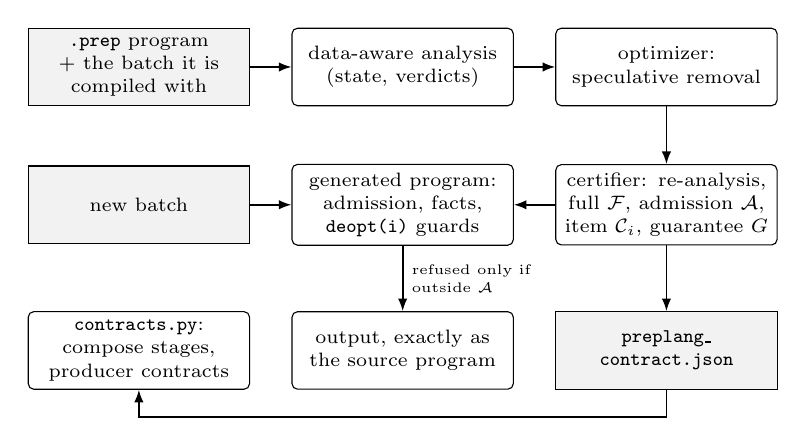
\begin{tikzpicture}[
    box/.style={draw, rounded corners=2pt, align=center, font={\fontsize{7}{8.4}\selectfont}, minimum height=2.8em,
                text width=2.6cm, inner sep=3pt},
    data/.style={draw, align=center, font={\fontsize{7}{8.4}\selectfont}, minimum height=2.8em, text width=2.6cm,
                 inner sep=3pt, fill=black!5},
    arr/.style={-{Latex[length=1.6mm]}, semithick},
    lbl/.style={font={\fontsize{5.5}{6.6}\selectfont}, align=left, inner sep=1pt}]
  \node[data] (src) at (0, 0) {\texttt{.prep} program\\+ the batch it is\\compiled with};
  \node[box] (ana) at (3.35, 0) {data-aware analysis\\(state, verdicts)};
  \node[box] (opt) at (6.7, 0) {optimizer:\\speculative removal};
  \node[box] (cer) at (6.7, -1.75) {certifier: re-analysis,\\full $\mathcal{F}$, admission $\mathcal{A}$,\\item $\mathcal{C}_i$, guarantee $G$};
  \node[box] (gen) at (3.35, -1.75) {generated program:\\admission, facts,\\\texttt{deopt(i)} guards};
  \node[data] (new) at (0, -1.75) {new batch};
  \node[box] (out) at (3.35, -3.6) {output, exactly as\\the source program};
  \node[data] (con) at (6.7, -3.6) {\texttt{preplang\_}\\\texttt{contract.json}};
  \node[box] (cmp) at (0, -3.6) {\texttt{contracts.py}:\\compose stages,\\producer contracts};
  \draw[arr] (src) -- (ana);
  \draw[arr] (ana) -- (opt);
  \draw[arr] (opt) -- (cer);
  \draw[arr] (cer) -- (gen);
  \draw[arr] (new) -- (gen);
  \draw[arr] (gen) -- node[lbl, right=2pt] {refused only if\\outside $\mathcal{A}$} (out);
  \draw[arr] (cer) -- (con);
  \draw[arr] (con.south) -- ++(0, -0.35) -| (cmp.south);
\end{tikzpicture}
\end{adjustbox}
\caption{How \PL compiles once and reuses the result. The certifier re-runs the analysis with weaker
input facts, reading no data; on a new batch, the generated program runs a removed instruction $i$
only if the batch breaks its item certificate $\mathcal{C}_i$.}
\label{fig:arch}
\end{figure}


Fig.~\ref{fig:students} cleans a table of students. Compiled against a file whose marks lie in
$[35,95]$ and whose names are all present, \PL proves the contracts on lines~2--3, finds that
\texttt{FILL\_NULL} on line~4 and \texttt{FILTER} on line~5 change nothing, and generates a program
without any of the four.

\begin{figure}[t]
\begin{lstlisting}
LOAD "students.csv" AS s;
EXPECT s.marks BETWEEN 0 AND 100;
EXPECT s.name NOT_NULL;
FILL_NULL s.marks WITH 0;
FILTER s WHERE marks >= 10;
SAVE s AS "out.csv";
\end{lstlisting}
\caption{A pipeline whose four statements on lines 2--5 the optimizer removes.}
\label{fig:students}
\end{figure}

\paragraph{Certificates.} The certifier analyses the program again with weaker facts: marks may be
missing, marks have no lower bound, and so on. A weakening is kept if the proofs survive. The
\emph{full certificate} keeps all four removals: marks in $[10,100]$ without missing values, names
without missing values, and the types of every column. Any batch inside it can run the optimized
program unchanged.

\paragraph{Deoptimization.} A batch with a mark of 101 is outside the full certificate. Without
deoptimization it must be refused. With it, the compiler has also found an \emph{item certificate}
per removal: the check on line~2 needs marks in $[0,100]$; the \texttt{FILL\_NULL} on line~4 needs
marks without missing values; the \texttt{FILTER} on line~5 needs marks of at least 10 without
missing values; the check on line~3 needs names. The \emph{admission certificate}, which keeps only
what no run-time code can stand in for, requires only the column types. The generated program keeps
the four statements behind guards, computes missing-value counts and ranges of the columns the
guards read, and for this batch re-enables only the check on line~2:
\begin{lstlisting}[language={},numbers=none]
Deoptimized line 2: EXPECT s.marks BETWEEN 0 AND 100:
  marks goes up to 101, above 100
ContractError: line 2: s.marks has values outside 0 to 100
\end{lstlisting}
The run stops exactly where a fresh compilation of the batch stops (it reports the contract as
violated). A batch with missing marks re-enables the fill and the filter, and writes what a fresh
compilation writes; a batch with marks as text is refused, because the compiled code reads marks as
integers. On 400 random batches, \RandFull{} fit the full certificate and \RandDeopt{} are admitted with
deoptimization; for every one of them, a fresh compilation proves every removal the program keeps
(Section~\ref{sec:eval}).

\paragraph{Composition.} The compiled program also states what \texttt{out.csv} satisfies for every
admitted batch: marks in $[10,100]$ without missing values (the deferred and re-enabled checks hold
whenever the run finishes). A second stage compiled on \texttt{out.csv} needs no admission check for
any fact that this guarantee implies, and \texttt{tools/contracts.py} names the facts it does not
imply, with the \texttt{EXPECT} that stage~1 would need.

\section{Data-Aware Compilation}\label{sec:lang}

\subsection{Language}
\PL programs are straight-line sequences of statements over tables (one CSV or Parquet file),
table sets (a folder of them), images, image sets, and images linked to a table of labels. Table
statements are \texttt{FILL\_NULL} (with a value, \texttt{MEAN}, \texttt{MEDIAN} or \texttt{MODE}),
\texttt{DROP\_NULL}, \texttt{NORMALIZE}, \texttt{FILTER} (with \texttt{AND}, \texttt{OR},
\texttt{NOT} and comparisons), \texttt{SELECT}, \texttt{DROP}, \texttt{PARSE\_DATE}, which turns a text
column of ISO dates into \textsc{DateTime}, and \texttt{DERIVE t.c = e}, which adds or replaces a
column computed with \texttt{+ - * /} from numeric columns and numbers, or as the \texttt{YEAR},
\texttt{MONTH}, \texttt{DAY}, \texttt{HOUR} or \texttt{WEEKDAY} of a date; image statements are
\texttt{RESIZE}, \texttt{GRAYSCALE}, \texttt{NORMALIZE RANGE}, \texttt{CONVERT}, \texttt{COMPRESS}
and \texttt{REMOVE\_CORRUPT}. Selectors such as \texttt{company.*.* WHERE TYPE NUMERIC} address many
columns, resolved against the inferred schemas. Contracts are written with \texttt{EXPECT}:
\texttt{NUMBER}, \texttt{STRING}, \texttt{BOOLEAN}, \texttt{NOT\_NULL}, \texttt{BETWEEN},
\texttt{UNIQUE}, \texttt{REFERENCES}, \texttt{SCHEMA\_SAME\_AS}, \texttt{CHANNELS},
\texttt{MIN\_WIDTH}, \texttt{MIN\_HEIGHT} and \texttt{MATCH\_RATE}. Every statement begins with its
own keyword, so the grammar is LL(1); the front end is a hand-written lexer and a recursive-descent
parser with panic-mode recovery. The compiler generates one Python program (pandas for tables,
OpenCV for images, one streaming pass per image save).

\subsection{The abstract dataset state}\label{sec:state}
The semantic analyzer maintains a state $\sigma$ mapping every dataset to an abstract value; a
single forward pass in the style of abstract interpretation~\cite{cousot1977} suffices, since
programs have no loops. For a table $T$ and column $c$, let $V_c(T)$ be the multiset of present
values and $M_c(T)$ the number of missing ones. A column is abstracted as
$a = \langle \tau, \nu, [l,u], \epsilon \rangle$: a type, $\nu \in \{\textit{none},
\textit{maybe}\}$ for missing values, an interval~\cite{cousot1976}, and an exactness flag, with
\begin{multline*}
\gamma(a) = \{\, T \mid V_c(T) \subseteq [l,u] \text{ with type } \tau,\;
  \nu = \textit{none} \Rightarrow M_c(T) = 0, \\
  \epsilon \Rightarrow \big(M_c(T) > 0 \Leftrightarrow \nu = \textit{maybe}\big) \wedge {} \\
  \big(V_c(T) = \emptyset \vee \min V_c = l \wedge \max V_c = u\big) \,\}.
\end{multline*}
An exact column promises that both bounds occur in the data, which is what allows a compile-time
\textsc{Violated} verdict. \texttt{LOAD} of a CSV file builds the exact state from every cell (a
parallel scanner analyses one million rows in \CsvMillion\,s, \CsvSpeedup$\times$ faster than
pandas reads them). An image set is abstracted as per-file shapes (width, height, channels, broken
or not) from the PNG or JPEG header, a pixel type, a pixel range and an output format. Transfer
functions follow the statements: \texttt{FILTER} refines intervals with its comparisons and, as in
SQL's three-valued logic~\cite{codd1979}, makes compared columns non-missing; \texttt{FILL\_NULL}
clears \textit{maybe} and joins the fill value; \texttt{NORMALIZE} sets $[0,1]$; \texttt{DERIVE}
computes the interval of its value by interval arithmetic and makes it \textit{maybe} missing where an
operand is; \texttt{RESIZE} sets every shape. \texttt{PARSE\_DATE} reads the values of its column (only
then, so no other program pays for it): if every value is a date in one ISO layout, the column becomes
\textsc{DateTime} with the first and last date as its interval, and otherwise the compiler names the
first row that is not a date. A part of a date has its full range (\texttt{MONTH} in $[1,12]$) unless
the dates fall in one year, month or day: dates from October to December give \texttt{MONTH} in
$[10,12]$, so a later \texttt{FILTER} on the month can be proven to keep every row. A division by a
value whose interval contains 0 is a compile error, since pandas would write infinities or missing
values without a word. Saves check that the format can hold the pixels: \textsc{Float32} pixels cannot
be saved as PNG, which a plain script would write as black images.

\paragraph{Metadata only.} For Parquet files~\cite{parquet,melnik2010} the compiler reads only the
footer: types from the schema, intervals from the per-row-group statistics that databases use as
zone maps~\cite{moerkotte1998}, missing values from the null counts. Compilation then costs
\PqSixteen\,s for one or 16 million rows; soundness rests on truthful writer statistics.

\subsection{Hybrid contract checking}\label{sec:contracts}
For a contract $\varphi$ at a point with state $\sigma$, the compiler returns \textsc{Proven} if
every dataset in $\gamma(\sigma)$ satisfies $\varphi$ (no check is generated), \textsc{Violated} if
none does (compilation fails, naming the first offending row), and \textsc{Deferred} otherwise (a
run-time check is generated). This is hybrid type checking~\cite{flanagan2006} and soft
typing~\cite{cartwright1991} applied to data. A deferred contract refines $\sigma$ afterwards,
because execution continues only if its check passed.

\begin{lemma}[Soundness of the analysis]\label{lem:sound}
If $T$ is the content of a CSV input, or of a Parquet input with truthful statistics, then
$T \in \gamma(\sigma_0)$; for every statement $s$, $T \in \gamma(\sigma) \Rightarrow
\llbracket s \rrbracket(T) \in \gamma(f_s(\sigma))$; a \textsc{Proven} verdict holds for every
$T \in \gamma(\sigma)$ and a \textsc{Violated} one for none.
\end{lemma}
\begin{proof}[Proof sketch]
The initial state is computed from all cells, or from statistics that bound the values; exactness is
claimed only when both bounds and the missing count are known. Transfer functions are case by case:
\texttt{FILTER} keeps a subset of rows that satisfy the condition and clears $\epsilon$;
\texttt{FILL\_NULL} adds its value exactly when values are missing. A \textsc{Violated} verdict needs
an exact column, whose bound is a value of the data.
\end{proof}

\paragraph{Optimizations.} Analysis results are attached to a three-address IR. \emph{Check
elimination} removes checks of proven contracts; \emph{no-effect elimination} removes a
\texttt{FILL\_NULL} on a column without missing values, a \texttt{FILTER} that is always true, a
\texttt{GRAYSCALE} of 1-channel images, a \texttt{RESIZE} to the size every image has;
\emph{column pruning} loads only live columns. All of them keep the output exact; the one
approximate rewrite (merging two resizes) runs only on request. Contracts proven by reading values
(\texttt{UNIQUE}, \texttt{REFERENCES}, \texttt{MATCH\_RATE}) keep a check that runs only when an
input differs from the compiled one.

\section{Data Certificates}\label{sec:cert}

Let $\sigma_0$ be the input state of the compiled files with every exactness flag cleared, so that it
describes a set of files rather than one. For an input state $\iota$, let $\Pi(\iota)$ be the set of
\emph{obligations} the analysis discharges from it: proven contracts and no-effect facts (each
identified by its statement and target), leaving out proofs that read the values, plus the absence
of compile errors. Order input states pointwise: $\textit{none} \sqsubseteq \textit{maybe}$,
interval inclusion, a fixed type, and for images per-file shapes inside boxes.

\begin{lemma}[Monotonicity]\label{lem:mono}
If $\iota' \sqsubseteq \iota$, then $\Pi(\iota') \supseteq \Pi(\iota)$.
\end{lemma}
\begin{proof}[Proof sketch]
Every decision is the inclusion of the state in a fixed predicate ($[l,u] \subseteq [a,b]$,
$\nu = \textit{none}$, a comparison true on all of $[l,u]$), which a smaller state keeps. Transfer
functions are joins and meets with constants; where a decision changes the path (a filter always
true in $\iota'$ but not in $\iota$, a contract proven in $\iota'$ but deferred in $\iota$), the
state of $\iota'$ is below the refined state of $\iota$ because it already satisfies the condition.
With exactness cleared, no verdict depends on a bound occurring in the data.
\end{proof}

A \emph{certificate} for a set of obligations $O$ is an input state $\cert{O}$ with
$O \subseteq \Pi(\cert{O})$. An input $T$ \emph{fits} it if $\alpha(T) \sqsubseteq \cert{O}$, where
$\alpha(T)$ is $T$'s own inexact state: every certified column has the type the compiler would infer,
no missing values where the certificate says \textit{none}, values inside the certified interval,
and every image file inside its box.

\begin{theorem}[Certificate soundness]\label{thm:cert}
If $T$ fits $\cert{O}$, every obligation in $O$ holds for $T$.
\end{theorem}
\begin{proof}
$\Pi(\alpha(T)) \supseteq \Pi(\cert{O}) \supseteq O$ by Lemma~\ref{lem:mono}; by
Lemma~\ref{lem:sound}, each proof derived from $\alpha(T)$ holds for $T$ at its program point, and
each removed operation does nothing there.
\end{proof}

\paragraph{Counterfactual re-analysis.} The certifier starts from $\sigma_0$ (first checking that it
still discharges what the compiled program used; otherwise only the exact files are admitted) and
weakens one fact at a time, running the whole analysis again: missing values are allowed; a lower
bound becomes $-\infty$, or else the loosest program constant below it that works, first as a closed
bound ($\geq k$) and then as an open one ($> k$); likewise upper bounds; a column the program only
carries to its output may be absent; image boxes gain channel counts and size ranges, again up to the
program's constants; the first and last date of a column \texttt{PARSE\_DATE} reads become open, or else
the start or end of their year, month or day; and that the column holds dates is kept or dropped like a
type. A weakening is kept if the criterion still holds. Without \texttt{DERIVE}, the analysis compares
intervals only with the program's constants, so no other bound can keep more and the result is
1-minimal (no remaining fact can be weakened on its own). A derived column compares values computed
from its inputs (\texttt{temp - 273.15 > 0}), and a part of a date changes at calendar boundaries; there
the result is maximal among the candidates, which include the numbers in \texttt{DERIVE}, but a bound
between them could keep more. Either way a rejected weakening tells which obligations need the
fact. The search uses the analysis as a black box, so it needs only a monotone forward analyzer, not
backward operators~\cite{mine2014}. When every obligation is a conjunction of conditions on single
facts of one column (range and not-null contracts, fills, and filters over one column are), the
certificates that discharge it form a product of chains, one per fact, and the search finds its
greatest element whatever the order in which facts are tried; an obligation over several columns,
such as a filter \texttt{a > 0 OR b > 0} that is always true, can have incomparable maximal
certificates (\texttt{a > 0}, or \texttt{b > 0}), and the order picks one. Each run reads no data: tables are replaced by their facts and
image folders by \emph{corner images}, one per combination of the extreme sizes, channel counts and
depths of the box. Every image decision is a universal or existential test over files of a
conjunction of one-dimensional conditions, so a folder inside the box passes whenever its corners do.

\paragraph{Every column.} The weakening runs over every column of the file, not only those the
optimized program loads: once \texttt{EXPECT t.id NOT\_NULL} is proven and pruning drops \texttt{id},
the certificate still requires it, and the generated program reads \texttt{id} only to check it.

\section{Selective Deoptimization}\label{sec:deopt}

The full certificate $\full = \cert{\Pi(\sigma_0)}$ treats every removal alike, so a batch that breaks
the fact behind one removed check is refused, although running that check would decide the batch
correctly. Dynamic compilers face the same choice with speculative code and resolve it by
deoptimization~\cite{holzle1992}. \PL applies it per batch and per removal.

\paragraph{Speculative removal.} The optimizer keeps every removed check and operation in the IR,
marked speculative (with the comparisons a removed \texttt{FILTER} needs). The certifier then finds,
one after the other and each starting from the previous result:
\begin{enumerate}
\item the \emph{full certificate} $\full$, for all of $\Pi(\sigma_0)$;
\item the \emph{admission certificate} $\adm$, for the obligations no run-time code can stand in
for: the absence of compile errors, contracts without a run-time check (types, image contracts),
and removals that cannot be re-enabled (a check of a column pruning dropped);
\item an \emph{item certificate} $\cert{i}$ for every speculative removal $i$, for the obligation
$\{i\}$ and the absence of errors, starting from $\full$.
\end{enumerate}
An item certificate is stored as the facts it needs beyond $\adm$; one that needs none is removed for
good. The generated program refuses a batch $T$ that does not fit $\adm$ (naming the fact and the
obligation), computes the missing-value count, minimum and maximum of the columns item certificates
mention (or the header facts of image folders), and runs each speculative instruction $i$ only if
$T$ does not fit $\cert{i}$:
\begin{lstlisting}[language=Python,numbers=none]
if deopt("2:1:s..marks"):
    if not df_s["marks"].dropna().between(0, 100).all():
        raise ContractError(
            "line 2: s.marks has values outside 0 to 100")
\end{lstlisting}
For the compiled file, \texttt{deopt} is false without looking at the data.

\begin{theorem}[Exact selective deoptimization]\label{thm:deopt}
Let $T$ fit $\adm$ and let $D = \{\, i \mid T \text{ does not fit } \cert{i} \,\}$. The generated
program with the removals outside $D$ skipped and those in $D$ run computes on $T$ exactly what the
source program computes: the same outputs, or a stop at the same check.
\end{theorem}
\begin{proof}
For $i \notin D$, $\alpha(T) \sqsubseteq \cert{i}$ and $i \in \Pi(\cert{i})$, so by
Lemma~\ref{lem:mono} $i \in \Pi(\alpha(T))$, and since $T$ fits $\adm$ no compile error occurs; by
Lemma~\ref{lem:sound} instruction $i$ does nothing at the state the source program reaches there on
$T$. Removing instructions that do nothing along a run does not change the run: by induction on the
program, the state before every remaining instruction is the same. The instructions in $D$ and all
others run as in the source program.
\end{proof}

\begin{corollary}[Agreement with a fresh compilation]
If a fresh compilation of $T$ succeeds, its program computes the same as the source program on $T$
(Lemma~\ref{lem:sound}), hence as the deoptimized program. If it reports a contract as violated, the
removal of that contract's check is not in $\Pi(\alpha(T))$, so it is in $D$ or was never removed;
the source program fails on $T$ at that check or at an earlier one, and so does the deoptimized
program.
\end{corollary}

So a batch is refused only for facts that no run-time code stands in for. Item certificates are
weaker than $\full$ in the directions their removal does not care about: the check on line~2 of
Fig.~\ref{fig:students} needs no lower bound of 10 and allows missing marks.

\paragraph{Mechanization.} We mechanized the theorem in Lean~4~\cite{lean4} in two layers, and a third
file proves Theorem~\ref{thm:cells} of Section~\ref{sec:private} for the core
(\texttt{proofs/}, \LeanLines{} lines of Lean's core language, no Mathlib; the theorems use only the axioms
\texttt{propext} and \texttt{Quot.sound}, which gives function extensionality, and no classical choice). \texttt{Deopt.lean} proves
Theorem~\ref{thm:deopt} for an abstract setting: a program is a list of partial state transformers; an
analysis is any function from abstract inputs to discharged obligations that is monotone and whose
no-effect proofs are sound for admitted inputs; item certificates are abstract inputs on which the
analysis discharges their removal; and the run-time check is sound for $\sqsubseteq$. It also proves
that the greedy search ends only on certificates the re-analysis accepted and that it only weakens.
\texttt{Core.lean} instantiates the setting with the analysis of a core of \PL: numeric columns
abstracted by $\nu$ and an interval, \texttt{FILL\_NULL}, \texttt{FILTER} with $\geq$ and $\leq$,
\texttt{DROP\_NULL}, \texttt{DERIVE} of the sum of two columns (interval addition), and \texttt{BETWEEN}
and \texttt{NOT\_NULL} contracts. For this core it proves the
transfer functions sound and every \textsc{Proven} verdict and no-effect proof valid
(Lemma~\ref{lem:sound}), monotonicity (Lemma~\ref{lem:mono}), the run-time check of the generated code
(missing values and bounds of the certified columns) sound and complete for a certificate, and from
these Theorem~\ref{thm:deopt} and the composition theorem of Section~\ref{sec:compose} end to end. For
the rest of the language (types, text, normalization, other arithmetic, dates, images, contracts
proven by reading values) the
two lemmas remain assumptions, which we test with randomized property tests that compare
deoptimization decisions with fresh compilations (Section~\ref{sec:soundtest}).

\section{Composing Pipeline Stages}\label{sec:compose}

Pipelines have stages: a cleaning stage writes a table that a feature stage reads. Each compiled
stage records, for every table it saves, the state the analysis computes at the \texttt{SAVE} when
its inputs are given the admission certificate: the stage's \emph{guarantee} $G$. Because selective
deoptimization keeps the source program's semantics (Theorem~\ref{thm:deopt}) and the analysis is
monotone, every file the stage writes for an admitted batch has its facts inside $G$; facts of
deferred contracts and of re-enabled checks hold because the run passed them.

\begin{theorem}[Composition]\label{thm:compose}
Let stage~2 read the table written by stage~1. If $G \sqsubseteq \cert{i}$ for a removal $i$ of
stage~2, stage~2 never deoptimizes $i$ for an output of stage~1 on an admitted batch; if
$G \sqsubseteq \adm_2$ on value facts, stage~2 never refuses such an output for its values.
\end{theorem}

The theorem is transitivity of $\sqsubseteq$ once the facts survive the file between the stages;
values and missing values do, while a type can change in a CSV round trip (a column whose values are
all missing reads back as text), so composition covers value facts and types are still checked on
admission, from metadata. \texttt{tools/contracts.py} reads the contract file every compilation
writes (\texttt{preplang\_contract.json}) and reports, for each fact stage~2 relies on, whether $G$
implies it; for each fact it does not, it writes the \texttt{EXPECT} statement that stage~1 would
need before its \texttt{SAVE}. Given several consumers of one table, it computes the conjunction of
their requirements: a \emph{producer contract}, synthesized from the consumers' code, under which no
consumer ever refuses or deoptimizes. Assume-guarantee reasoning is standard for component
contracts~\cite{benveniste2018}, and schema registries check the containment of writer and reader
schemas~\cite{avro}; here the contracts on both sides are derived from the stages' proofs.

\section{Compiling Against Data You Cannot See}\label{sec:private}

A data-aware compiler leaks its data through what it writes. The generated program embeds the
checksum of the compiled file, which confirms a guessed file; every removal states a fact about it
(no value of \texttt{age} is missing, no mark is below~10); a violated contract names a row; the
contract file records bounds. Yet programs travel further than data: in validation
servers~\cite{barrientos2018} and platforms such as OpenSAFELY~\cite{williamson2020}, an analyst writes
code for confidential records against dummy data, and the data owner runs it on the real ones. The
analyst needs what a data-aware compiler gives (which fills are needed, which contracts the data
breaks, which filters do nothing) and may not see the data that produces it.

\paragraph{Guards are necessary.} The facts such a compiler needs are \emph{emptiness} facts: no value
is missing, no value is below $k$. No differentially private release can certify one. If a mechanism
$M$ is $\varepsilon$-differentially private and a table $D'$ differs from $D$ in $k$ rows that break
the fact, then $\Pr[M(D') = o] \ge e^{-k\varepsilon}\Pr[M(D) = o]$ for every output $o$: whatever $M$
says on a clean table it also says, with comparable probability, on a table that breaks the fact in a
few rows. One-sided noise keeps differentially private query processing exact when it decides how
many padding tuples to drop~\cite{bater2018,wang2024special}, up to the failure probability $\delta$ of
approximate differential privacy; it cannot make an \emph{unguarded} removal safe, because a removal
needs the emptiness fact itself. A program optimized from released emptiness facts must check them on
the data it runs on. Selective deoptimization does exactly that. Theorem~\ref{thm:deopt} has no
hypothesis about the facts the compiler starts from (in Lean, \texttt{deopt\_correct} quantifies over
arbitrary removals and certificates): the facts decide which instructions are removed speculatively and
which certificates guard them, and the generated program checks the certificates on the batch. A
wrong fact costs a deoptimization, never a wrong result.

\paragraph{What the analysis needs.} Which questions should the owner answer? Exactly those the
analysis asks.

Let $K$ be the numbers a program compares columns with, together with~0, and let
$k_1 < \dots < k_m$ be its elements. They cut a numeric column into the $2m+2$ \emph{cells}
$(-\infty,k_1)$, $\{k_1\}$, $(k_1,k_2)$, \ldots, $\{k_m\}$, $(k_m,\infty)$ and \emph{missing}; any other
column has two cells, \emph{value} and \emph{missing}. A table \emph{occupies} a cell of a column if some
row's value lies in it.

\begin{theorem}[Cells]\label{thm:cells}
Let a program over tables with a declared schema have no \texttt{DERIVE} and no \texttt{PARSE\_DATE}, and
no contract that reads values (\texttt{UNIQUE}, \texttt{REFERENCES}, \texttt{MATCH\_RATE}). Two tables
that occupy the same cells of every column receive the same verdicts and the same removals from the
analysis.
\end{theorem}
\begin{proof}[Proof sketch]
Every decision compares a bound with a number of $K$, and every transfer function raises, lowers or
joins a bound with a number, which keeps two states that agree on all comparisons with $K$ in agreement:
$\textit{lo}\,(\textit{raise}(l, k_0)) \ge k$ holds exactly when $l \ge k$ or $k_0 \ge k$, and likewise for
the other functions. For a table's own facts, ``the minimum is at least $k$'' is the question ``some value
exists and none is below $k$'', and ``the minimum is above $k$'', which a strict comparison or \texttt{==}
asks, adds ``none is $k$''. The types are declared, so they do not depend on the values.
\end{proof}

The hypotheses are needed. Ids $\{1,2\}$ and $\{1,1\}$ occupy the same cells, but only the first satisfies
\texttt{UNIQUE}; and the ages $\{10,29\}$ and $\{10,30\}$ agree on ``a value below 30'' and ``a value above
30'' but not on the point cell $\{30\}$, which decides whether \texttt{FILTER s WHERE age < 30} removes a
row. We mechanized the theorem for the core in Lean (\texttt{cells\_decide} in \texttt{proofs/Cells.lean},
\LeanCellsLines{} lines, axioms \texttt{propext} and \texttt{Quot.sound}); the core has only $\ge$ and $\le$,
for which ``a value below $k$'' and ``a value above $k$'' suffice. For the compiler, a randomized test
compiles one program (two contracts, a fill, a filter with a strict comparison, a \texttt{DROP\_NULL}) for
\PrivCellPairs{} pairs of different integer tables that occupy the same cells (other values, other row
counts, other orders) and finds identical verdicts, removals, speculative instructions and certificates
for every pair. Two consequences. First, the occupied cells are \emph{all} the analysis can use: released
exactly, they give a private compilation the normal compilation's removals (RQ8 confirms this on every
workload), so a differentially private release of them loses nothing but its noise. Second, the
\emph{decisions} of a normal compilation of such a program (its verdicts, removals and speculative
instructions) reveal at most $2|K|+2$ bits per numeric column, which cells are occupied. The rest of what
a normal compilation writes reveals more: the checksum, the inferred types, the messages, which quote
values, and the bounds recorded in the contract file and the output guarantees. A private compilation
drops these or computes them from the release.

\paragraph{What is released.} The data owner runs the compiler with \texttt{--queries}, which writes
the schema of each input (names and types of its columns) and the numbers written in the program. The
analysis compares bounds only with these numbers (Section~\ref{sec:cert}): for a program without
\texttt{DERIVE}, the numbers $k_1 < \dots < k_m$ (and~0) cut a column into the cells
$(-\infty,k_1)$, $\{k_1\}$, $(k_1,k_2)$, \ldots, $\{k_m\}$, $(k_m,\infty)$ and \emph{missing}, and every
decision depends only on which cells hold some row. \texttt{tools/release\_facts.py} releases one
Laplace histogram over these cells per column~\cite{dwork2014}: a row lies in exactly one cell of a
column, so the histogram has sensitivity~1. Only columns the program names are asked about (all if it
uses \texttt{*} or a \texttt{DROP\_NULL} of whole rows), and of those only missing values unless they
are numeric. Each table gets the whole budget $\varepsilon$, divided equally between its columns
asked about. A cell counts as occupied if its noisy count is above $t + \frac12$ with
$t = \ln(C/\beta)/\varepsilon_c$, where $C$ is the number of cells released and $\varepsilon_c$ the
budget of the cell's column. A column's facts are read off its occupied cells: missing values if the missing
cell is occupied; bounds from the lowest and highest occupied value cells; and, as evidence, that values
below the upper edge of the lowest occupied cell (or above the lower edge of the highest) exist.

\begin{theorem}[Privacy]\label{thm:private}
For a schema fixed independently of the data, the facts file is $\varepsilon$-differentially private for
adding or removing one row of any input table, and so is everything the compiler writes for the
analyst: the generated program, the certificates, the contract file, the manifest and every message.
\end{theorem}
\begin{proof}
A Laplace histogram with noise $\mathrm{Lap}(1/\varepsilon_c)$ per cell and sensitivity~1 is
$\varepsilon_c$-differentially private. A row is in every column of its table, so those columns compose
sequentially, with $\sum \varepsilon_c = \varepsilon$ per table; a neighbouring dataset differs in one
row of one table, so the tables compose in parallel. Which columns and cells are asked about depends
only on the program and the schema, never on an answer, so the composition is non-adaptive. The occupied cells, the facts, the evidence and the compiler's outputs are computed from
the noisy histograms, the program and the schema alone; the compiler never opens an input file
(\texttt{--facts} fails rather than read a table without released facts).
\end{proof}

\paragraph{People, not rows.} A person with $g$ rows is protected only at $g\varepsilon$ by a release that
protects rows. With \texttt{--unit} the owner names the column that identifies a person in every table;
at most $m$ rows of each unit are counted (the first $m$ in file order) and rows without a unit are not
counted, so adding or removing a whole unit changes each count by at most $m$. The noise is
$\mathrm{Lap}(m/\varepsilon_c)$ and the threshold $t = m\ln(C/\beta)/\varepsilon_c$, and since a unit may have
rows in every table, all columns of all tables share $\varepsilon$; the release is then
$\varepsilon$-differentially private for adding or removing a unit. Contribution bounding is standard
in differentially private systems~\cite{wilson2020}, where the rows it drops bias every answer. Here
the bias never costs exactness: a fact that the truncation makes false is one of the facts the generated
program checks on the real data, and a run deoptimizes it. It does cost what the analyst learns, as noise
does: fewer removals are justified and fewer warnings are given (Section~\ref{sec:rq-private}).

The hypothesis on the schema is not a formality. A type the compiler \emph{infers} is a fact about the
values: a CSV column is \textsc{Integer} until one cell holds 3.5, and pandas writes an integer column
with a missing value to Parquet as a float column. \texttt{--queries} writes the inferred types as the
owner's draft; the owner must publish the schema as declared (a data dictionary), not as found. The seed
of the noise is never written to the facts file: whoever knows it can recompute the noise.

\begin{theorem}[Exactness for any facts]\label{thm:anyfacts}
For any facts file, true, noisy or false, the generated program computes on every batch it admits
exactly what the source program computes.
\end{theorem}
\begin{proof}
Without a checksum, no batch is treated as the compiled one: every batch, including the file the
facts describe, is checked against the admission and item certificates. Theorem~\ref{thm:deopt}
applies unchanged.
\end{proof}

\paragraph{What the analyst sees of a run.} On a validation server the analyst learns at least
whether a job finished. If a released fact could make the generated program refuse a batch, an
analyst who chooses the program's numbers could learn a bit about one row from each submission. So
no released fact enters the admission certificate: in a private compilation a removed check keeps its
column loaded (a normal compilation prunes the column and makes the check's proof an admission fact),
so every removal can run again. The admission facts that remain are the declared types and the
absence of compile errors.

\begin{corollary}[Outcomes do not depend on the facts]\label{cor:outcome}
Let the program not divide in \texttt{DERIVE}. For a declared schema, the programs generated from any two
facts files refuse the same batches, those that break a declared type, and on every other batch both
compute what the source program computes. Of a run, the released facts change only which removed
instructions run again, that is, how long it takes.
\end{corollary}
\begin{proof}
The admission certificate holds the declared types, the facts that keep the program free of compile
errors, and the proofs no run-time code stands in for. In a private compilation nothing is exact, so no
contract is reported violated; contracts on types and schemas are decided by the declared schema; and
\texttt{PARSE\_DATE}, images and folders of tables are refused whatever the facts. The one compile error
left that depends on bounds is a division in \texttt{DERIVE} by an expression whose range contains~0,
which the hypothesis excludes. A removed check keeps its column loaded, so every removal can run again
and no proof needs admission. The admission certificate is therefore the same for every facts file, and every other fact
guards a removal that runs again when broken (Theorem~\ref{thm:anyfacts}).
\end{proof}

\begin{lemma}[What the analyst learns]\label{lem:utility}
With probability at least $1-\beta$ over the noise, for every released cell: (i) if it is occupied, it
holds at least one row; and (ii) if it holds at least $2t + 1$ rows, it is occupied. Hence every
``likely violated'' warning names a contract the data breaks; for a program without \texttt{DERIVE}
whose columns each have an occupied value cell, every released bound is at or inside the tightest true
bound at the program's numbers (an occupied cell holds a row), so the private compilation removes at
least what a normal compilation of
the same file removes (except checks of \texttt{UNIQUE} and \texttt{REFERENCES}, which read values); and
a released fact is false only if fewer than $c(2t + 1)$ rows break it, where $c$ is the number of cells
it covers ($c = 1$ for ``no missing values'').
\end{lemma}
\begin{proof}
$\Pr[|\mathrm{Lap}(1/\varepsilon_c)| > t] = e^{-\varepsilon_c t} = \beta/C$, so by a union bound every
noise is at most $t$ with probability $1-\beta$. Then a noisy count above $t + \frac12$ has a true count
above $\frac12$, and a true count of at least $2t+1$ gives a noisy count of at least $t+1$. A column with
no occupied value cell gets no bounds at all, which is why the hypothesis is needed. The removals follow
from Lemma~\ref{lem:mono}, because decisions compare bounds only with the program's numbers.
\end{proof}

The bound in the last part is what separates the release from the \emph{optimistic} facts ``nothing is
missing'', which need no data and also give every removal of a normal compilation. False facts cost
deoptimizations, and Theorem~\ref{thm:anyfacts} keeps every admitted run exact. In a normal
compilation a false admission fact (the proven check of a column the optimized program does not load)
would instead refuse batches; a private compilation keeps such checks (Corollary~\ref{cor:outcome}). The
mechanized core does not cover admission (its admission predicate is true), types or compile errors;
those parts are tested. Because the release depends only on which cells are occupied, one release can serve
several programs over the same files: the cells of their numbers together are released once, and each
program reads its facts off them. A private compilation cannot report a contract as violated, since
nothing it knows is exact and a row would name a person; a contract the released evidence shows broken
gets a warning (``\texttt{EXPECT s.marks BETWEEN 0 AND 100} is likely violated: the released facts
report values of \texttt{s.marks} above 100''), and the check runs on the real data. Contracts that read
the values (\texttt{UNIQUE}, \texttt{REFERENCES}) are always checked at run time. A fact about a few rows,
such as two missing \texttt{Embarked} values among 891 passengers, is hidden by design; the run-time check
covers it. Images, folders of tables and \texttt{PARSE\_DATE}, which read values or file lists, are not
supported in a private compilation. The guarantee covers what the compiler writes: what the owner's runs
print (a deoptimization names a row) and how long they take stay with the owner, and releasing them would
need a mechanism of its own.

\section{Lifting pandas Scripts}\label{sec:lift}

Certificates are most useful for code that already exists. A second front end parses a pandas script
with Python's own parser, follows every DataFrame read with \texttt{pd.read\_csv(path)}, and
translates, in order, the statements that change a followed DataFrame in a way \PL expresses:
\texttt{fillna} with a constant or the column's \texttt{mean()}, \texttt{median()} or
\texttt{mode()[0]}; \texttt{dropna}; \texttt{drop} of columns; column selection; boolean-mask
filters; min--max and z-score normalization written as arithmetic; \texttt{assert} with
\texttt{between}, \texttt{notna} or \texttt{is\_unique}; and \texttt{to\_csv}. A second version,
written after the corpora of Section~\ref{sec:rq-corpus} were evaluated, also translates
\texttt{pd.to\_datetime} of a column into \texttt{PARSE\_DATE} (with \texttt{errors="coerce"}, too:
on the inputs \PL admits, both read the same dates), \texttt{.dt.hour} and the other date parts, and
arithmetic over columns and numbers into \texttt{DERIVE}. Statements that only read a DataFrame are
skipped. Lifting stops at the first statement that changes a DataFrame in another way (\texttt{map},
\texttt{get\_dummies}, \texttt{set\_index}): the result is the longest prefix of the script's cleaning
that \PL expresses exactly. The lifted statements, run on their own, are the ground truth for the
compiled program in Section~\ref{sec:eval}.

\section{Implementation}
The compiler is about \SrcLines{} lines of C++17 without external libraries: lexer, parser, schema
provider (parallel CSV scanner, a Thrift compact-protocol reader for Parquet footers, PNG and JPEG
header readers), semantic analyzer, IR, pass manager, certifier, and an execution planner over the
pandas and OpenCV code generators. Every compilation writes the generated program, a manifest, and the
contract file. The front end for pandas, the composition tool and the evaluation harness are Python;
the unit tests (\TestCount{} checks in \TestSuites{} suites) include the randomized soundness tests.

\section{Evaluation}\label{sec:eval}

We ask seven questions. \textbf{RQ1:} Does compiling against the data find mistakes before any data
is processed? \textbf{RQ2:} What does data-aware compilation cost and gain? \textbf{RQ3:} Can a
compiled program be reused on edited batches? \textbf{RQ4:} On real data that changes from month to
month, compared with data-validation tools? \textbf{RQ5:} For real pandas scripts? \textbf{RQ6:} Do
certificates compose across stages? \textbf{RQ7:} What do certification and reuse cost? We also report
how we tested soundness and the bugs the evaluation found in our own implementation.

\paragraph{Setup.} Intel Core i5-12450H (8 cores), 16\,GB RAM, Windows~11; MSVC 14.44 (Release);
Python 3.14, pandas 3.0, NumPy 2.5, OpenCV 5.0, pyarrow 25. pandera 0.34 and Great Expectations
0.18.22, whose onboarding data assistant builds a suite from a sample (we found no such assistant in
the 1.x line), run in a Python 3.11 environment, TFDV 1.21 in WSL (Ubuntu, Python 3.12), since it has
no Windows build. Times include starting Python.

\paragraph{Scoring reuse.} RQ3--RQ6 score every way of running a new batch $T$ against the ground
truth: a fresh compilation of the pipeline for $T$, run. A policy either runs a program on $T$ or
refuses it. Its outcome is \emph{correct} if it wrote exactly the files of the fresh run or stopped
where the fresh run stops (a refusal, or a failing check, when the fresh compilation fails or its run
stops); \emph{needless} if it refused $T$ although the fresh compilation runs, which costs a
recompilation; and \emph{wrong} if it finished with other files than the fresh run, finished where the
fresh run fails, or stopped where it does not. The policies are: the \emph{fingerprint} of the
compiled file; the compiled file's own facts (types, no missing values, and the range of every column
read, a schema as TFDV would record it with ranges); pandera's \texttt{infer\_schema} (dtypes,
nullability, numeric ranges); Great Expectations' onboarding data assistant (an inferred suite of
column statistics); TFDV's \texttt{infer\_schema} (types, presence, string domains); the \emph{full
certificate}; and \emph{selective deoptimization}. The validators are set up on the file the pipeline
was compiled with, once on every column (as they are used) and once on the columns the program reads
(more favourable to them); when a validator admits $T$, the optimized program runs on it as it is.

\subsection{RQ1: Mistakes found before any data is processed}

\paragraph{Injected mistakes.} We injected 24 mistakes into the five example programs, one per
mutant~\cite{jia2011}: misspelled columns, type errors (normalizing text, comparing a number with
text), uses after removal, broken contracts (range, not-null, foreign key, schema, channels, width,
match rate), a broken image, and three well-typed programs with silently wrong output. \PL reports all
24 at compile time and nothing on the unmodified programs, in \RqOneMsMin--\RqOneMsMax\,ms; a
script-style interpreter of the same programs crashes part-way on 20 and finishes 4 with wrong output
(text filled into an integer column, a threshold on a normalized column that removes every row, and
two pipelines that write black images). On 16 million Parquet rows, a misspelled column is reported in
\ScTabNamePl\,s instead of after \ScTabNameScript\,s, and float pixels saved as PNG in \ScImgFloatPl\,s
for 3,000 images, where the script runs \ScImgFloatScript\,s and writes black images.

\paragraph{Real failures.} We chose 17 error messages that Python libraries print for common
data-preparation failures, searched GitHub issues for each and read the first 12 results in order; an
issue qualified if the failure happened while loading, transforming or saving data files and its root
cause was stated, at most three per message: \RbTotal{} issues~\cite{islam2019,humbatova2020}. \PL
reports \RbEarly{} of them (\RbEarlyPct\%) before any data is processed (\RbCompile{} without
annotation, \RbContract{} once the requirement is declared with \texttt{EXPECT}); \RbDesign{} cannot
occur in a \PL program, and \RbNone{} are not covered (input formats such as HEIC or GeoTIFF,
operations such as pivots, dates, per-image label files). \RbPass{} of \RbCases{} reproductions behave
as classified.

\subsection{RQ2: Cost and gain of data-aware compilation}

Analysing every cell of a one-million-row CSV file takes \CsvMillion\,s, \CsvSpeedup$\times$ faster
than pandas' default reader reads it; Parquet compilation stays at \PqSixteen\,s from one to 16
million rows; reading 3,000 image headers is \HdrRatio$\times$ faster than decoding the images. On a
200,000-row, 40-column table with two contracts and a filter, the optimizer proves both contracts and
loads 5 of 40 columns; the optimized program processes the data in \TabProcOpt\,s instead of
\TabProcOz\,s (\TabCut\% less) with byte-identical output. Image pipelines stream one image at a
time, in \ImgPlMem\,MiB of memory instead of \ImgBaseMem\,MiB for loading all 1,000 images.

\subsection{RQ3: Reusing a compiled program on edited batches}\label{sec:rq-edits}

Seven workloads are compiled once: the four table examples, one program run twice on one file, the
Parquet example, images linked to labels, and a sensor pipeline of 20,000 rows per day. Each input
table gets new batches: other days and a warmer season of the sensor process, and, for the examples,
rows resampled with replacement, values moved by noise of 0.1, 0.5 and 1.5 standard deviations, 20\%
missing values in one column, and one value far out of range (\CertBatches{} batches).

\begin{table*}[t]
\caption{Reusing compiled programs on edited batches (RQ3): per policy, batches handled correctly (ok: the fresh files, or a stop where the fresh run stops), refused although a fresh compilation runs (ref.), and finished with other files or where the fresh run fails (wrong).}
\label{tab:rq-edits}
\centering
\footnotesize
\begin{adjustbox}{max width=\linewidth}
\begin{tabular}{@{}lrrrrrrrrr@{}}
\toprule
& \multicolumn{3}{c}{tables} & \multicolumn{3}{c}{images + labels} & \multicolumn{3}{c}{all} \\
\cmidrule(l){2-4}\cmidrule(l){5-7}\cmidrule(l){8-10}
Policy & ok & ref. & wrong & ok & ref. & wrong & ok & ref. & wrong \\
\midrule
Fingerprint & 98 & 126 & 0 & 17 & 3 & 0 & 115 & 129 & 0 \\
File facts & 121 & 78 & 25 & 1 & 3 & 16 & 122 & 81 & 41 \\
pandera, every column & 120 & 79 & 25 & 1 & 3 & 16 & 121 & 82 & 41 \\
pandera, columns read & 123 & 76 & 25 & 1 & 3 & 16 & 124 & 79 & 41 \\
Great Expectations, every column & 121 & 103 & 0 & 17 & 3 & 0 & 138 & 106 & 0 \\
Great Expectations, columns read & 123 & 101 & 0 & 17 & 3 & 0 & 140 & 104 & 0 \\
TFDV, every column & 146 & 28 & 50 & 1 & 3 & 16 & 147 & 31 & 66 \\
TFDV, columns read & 149 & 25 & 50 & 1 & 3 & 16 & 150 & 28 & 66 \\
Full certificate & 224 & 0 & 0 & 20 & 0 & 0 & 244 & 0 & 0 \\
\textbf{Selective deoptimization} & \textbf{224} & \textbf{0} & \textbf{0} & \textbf{20} & \textbf{0} & \textbf{0} & \textbf{244} & \textbf{0} & \textbf{0} \\
\bottomrule
\end{tabular}
\end{adjustbox}
\end{table*}


Both certificates handle every batch correctly (Table~\ref{tab:rq-edits}): the full certificate by
refusing exactly the batches whose fresh compilation fails, selective deoptimization by running them
and stopping at the re-enabled check (\CertDeopted{} batches ran with removals re-enabled). The
fingerprint refuses every edited batch (\CertFpNeedless{} of them needlessly), and the compiled file's
own facts refuse \CertFactsNeedless{} that a fresh compilation runs. Gating the
optimized program with the file's own facts is also unsound (\CertFactsUnsound{} wrong runs): on the
table set and on the linked images, resampled and drifted rows repeat keys or lose matches, so a
contract the compiler had proven by reading the values (\texttt{UNIQUE}, \texttt{REFERENCES},
\texttt{MATCH\_RATE}) no longer holds and the fresh compilation reports it, while the file's facts,
which are facts of single columns, admit the batch and the optimized program finishes. \PL runs such
checks again whenever an input changed. The real validators fare no better: pandera's inferred schema
is unsound on the same batches (\CertPanderaAllUnsound{} wrong), TFDV's, which has no ranges, on these
and on batches whose values drift past what a removed check or filter relied on (\CertTfdvAllUnsound{}
wrong), and Great Expectations' statistical suite, which
is sound here, refuses \CertGxAllNeedless{} batches that a fresh compilation runs.

\paragraph{Image folders.} A pipeline that makes images gray and $64\times64$, compiled on a folder
of gray $64\times64$ images, has its \texttt{GRAYSCALE} and \texttt{RESIZE} removed speculatively. We
gave it \ImgBatches{} new folders: gray $64\times64$ images, some color images, other sizes, both, a
file that is not an image, and 16-bit images (five each), and compared the written images byte by
byte with a fresh compilation. Selective deoptimization handles \ImgBDeoptCorrect{} correctly,
re-running \texttt{GRAYSCALE} or \texttt{RESIZE} on \ImgBDeopted{} folders; the full certificate
refuses those folders, and the optimized program run on them without a check writes color or
wrongly sized images (\ImgBTrustedUnsound{} folders). The \ImgBDeoptNeedless{} needless refusals are
the 16-bit folders: bit depths are fixed in every certificate because they decide the pixel type the
generated code assumes, even where, as here, no instruction depends on it; certifying them would need
the code generator's assumptions as obligations too.

\subsection{RQ4: Real monthly data, against data-validation tools}\label{sec:rq-real}

Three public datasets come in monthly batches: hourly traffic and weather on a Minnesota interstate
(UCI, 2012--2018, 63 months of CSV), daily bike rentals in Washington (UCI, 2011--2012, 24 months),
and New York green-taxi trips (NYC TLC, 2022--2024, the 36 Parquet files as published). For each we
wrote one cleaning pipeline as a data engineer would: range contracts on the measured quantities,
\texttt{NOT\_NULL} on keys, fills, a filter that removes impossible readings, a normalization and a
selection. Each pipeline is deployed twice: compiled on the first month and run on every later one,
and compiled on the month before each month (\RealRuns{} runs; twice the month before has a temperature of
0\,K, fails to compile itself, and leaves nothing to deploy). Batches are cut from the raw
files, so no value is reformatted.

\begin{table*}[t]
\caption{Reusing compiled pipelines on real monthly batches (RQ4), both deployments (compiled on the first month, and on the month before). ok: handled as a fresh compilation of the month would; ref.: refused although a fresh compilation runs; wrong: finished with other files than the fresh run, or where it fails. Validators gate the optimized program (Section~\ref{sec:rq-real}).}
\label{tab:rq-real}
\centering
\footnotesize
\begin{adjustbox}{max width=\linewidth}
\begin{tabular}{@{}lrrrrrrrrrrrrrrrrrr@{}}
\toprule
& \multicolumn{3}{c}{Traffic (CSV)} & \multicolumn{3}{c}{Bikes (CSV)} & \multicolumn{3}{c}{Taxi (Parquet)} & \multicolumn{3}{c}{Citi Bike (CSV)} & \multicolumn{3}{c}{Air quality (CSV)} & \multicolumn{3}{c}{all 426} \\
\cmidrule(l){2-4}\cmidrule(l){5-7}\cmidrule(l){8-10}\cmidrule(l){11-13}\cmidrule(l){14-16}\cmidrule(l){17-19}
Policy & ok & ref. & wrong & ok & ref. & wrong & ok & ref. & wrong & ok & ref. & wrong & ok & ref. & wrong & ok & ref. & wrong \\
\midrule
Fingerprint & 3 & 119 & 0 & 0 & 46 & 0 & 14 & 56 & 0 & 0 & 70 & 0 & 0 & 118 & 0 & 17 & 409 & 0 \\
File facts & 5 & 117 & 0 & 0 & 46 & 0 & 14 & 56 & 0 & 0 & 70 & 0 & 0 & 118 & 0 & 19 & 407 & 0 \\
pandera, every column & 5 & 117 & 0 & 0 & 46 & 0 & 14 & 56 & 0 & 0 & 70 & 0 & 0 & 118 & 0 & 19 & 407 & 0 \\
pandera, columns read & 5 & 117 & 0 & 0 & 46 & 0 & 14 & 56 & 0 & 0 & 70 & 0 & 0 & 118 & 0 & 19 & 407 & 0 \\
Great Expectations, every column & 3 & 119 & 0 & 0 & 46 & 0 & 14 & 56 & 0 & 0 & 70 & 0 & 0 & 118 & 0 & 17 & 409 & 0 \\
Great Expectations, columns read & 3 & 119 & 0 & 0 & 46 & 0 & 14 & 56 & 0 & 0 & 70 & 0 & 0 & 118 & 0 & 17 & 409 & 0 \\
TFDV, every column & 5 & 117 & 0 & 0 & 46 & 0 & 63 & 0 & 7 & 13 & 57 & 0 & 49 & 69 & 0 & 130 & 289 & 7 \\
TFDV, columns read & 92 & 27 & 3 & 0 & 46 & 0 & 63 & 0 & 7 & 13 & 57 & 0 & 49 & 69 & 0 & 217 & 199 & 10 \\
Full certificate & 120 & 2 & 0 & 44 & 2 & 0 & 68 & 2 & 0 & 50 & 20 & 0 & 115 & 3 & 0 & 397 & 29 & 0 \\
\textbf{Selective deoptimization} & \textbf{122} & \textbf{0} & \textbf{0} & \textbf{46} & \textbf{0} & \textbf{0} & \textbf{70} & \textbf{0} & \textbf{0} & \textbf{70} & \textbf{0} & \textbf{0} & \textbf{118} & \textbf{0} & \textbf{0} & \textbf{426} & \textbf{0} & \textbf{0} \\
\bottomrule
\end{tabular}
\end{adjustbox}
\end{table*}

\begin{figure}[t]
\centering
\begin{adjustbox}{max width=\linewidth}
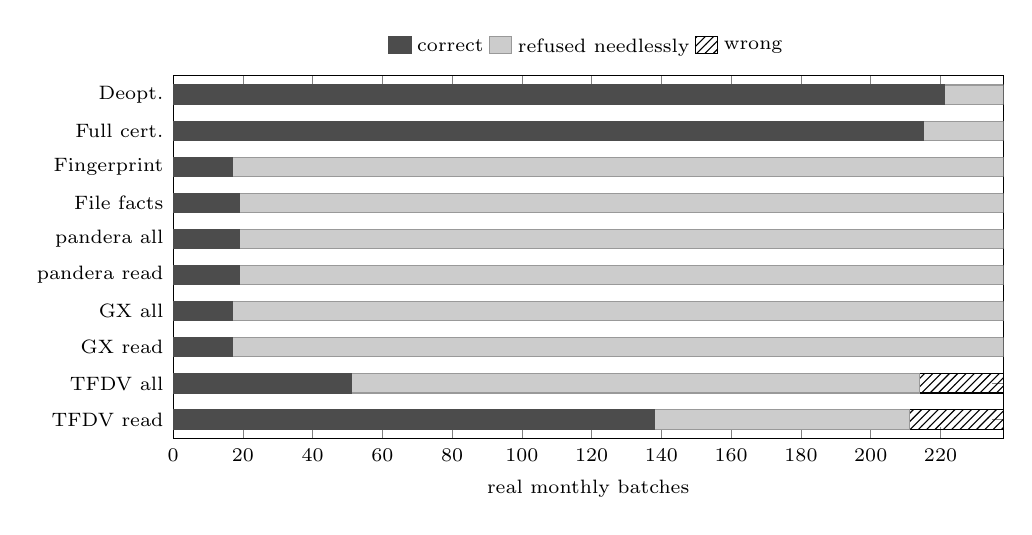
\begin{tikzpicture}
\begin{axis}[
    xbar stacked, bar width=7pt, width=\columnwidth, height=6.2cm,
    xmin=0, xmax=\RealRuns, enlarge y limits=0.06,
    xlabel={real monthly batches}, xlabel style={font=\scriptsize},
    symbolic y coords={TFDV read,TFDV all,GX read,GX all,pandera read,pandera all,File facts,Fingerprint,Full cert.,Deopt.},
    ytick=data, yticklabel style={font=\scriptsize}, xticklabel style={font=\scriptsize},
    legend style={font=\scriptsize, at={(0.5,1.02)}, anchor=south, legend columns=3, draw=none},
    reverse legend=false]
\addplot[fill=black!70, draw=black!70] coordinates {
    (\RealTfdvReadCorrect,TFDV read) (\RealTfdvAllCorrect,TFDV all) (\RealGxReadCorrect,GX read)
    (\RealGxAllCorrect,GX all) (\RealPanderaReadCorrect,pandera read) (\RealPanderaAllCorrect,pandera all)
    (\RealFactsCorrect,File facts) (\RealFpCorrect,Fingerprint) (\RealFullCorrect,Full cert.)
    (\RealDeoptCorrect,Deopt.)};
\addplot[fill=black!20, draw=black!40] coordinates {
    (\RealTfdvReadNeedless,TFDV read) (\RealTfdvAllNeedless,TFDV all) (\RealGxReadNeedless,GX read)
    (\RealGxAllNeedless,GX all) (\RealPanderaReadNeedless,pandera read) (\RealPanderaAllNeedless,pandera all)
    (\RealFactsNeedless,File facts) (\RealFpNeedless,Fingerprint) (\RealFullNeedless,Full cert.)
    (\RealDeoptNeedless,Deopt.)};
\addplot[pattern=north east lines, pattern color=black, draw=black] coordinates {
    (\RealTfdvReadUnsound,TFDV read) (\RealTfdvAllUnsound,TFDV all) (\RealGxReadUnsound,GX read)
    (\RealGxAllUnsound,GX all) (\RealPanderaReadUnsound,pandera read) (\RealPanderaAllUnsound,pandera all)
    (\RealFactsUnsound,File facts) (\RealFpUnsound,Fingerprint) (\RealFullUnsound,Full cert.)
    (\RealDeoptUnsound,Deopt.)};
\legend{correct, refused needlessly, wrong}
\end{axis}
\end{tikzpicture}
\end{adjustbox}
\caption{RQ4: \RealRuns{} real monthly batches, by admission policy. \emph{Correct}: ran and wrote
the fresh compilation's files, or stopped where it stops; \emph{refused needlessly}: a recompilation
was needed although the fresh compilation runs; \emph{wrong}: other files, or a run where the fresh
compilation fails. Validators gate the optimized program; \emph{all}/\emph{read}: set up on every
column, or on the columns the program reads.}
\label{fig:policies}
\end{figure}

\begin{figure*}[t]
\centering
\definecolor{deopt}{RGB}{217,95,2}
\begin{adjustbox}{max width=\linewidth}
\begin{tikzpicture}[font=\scriptsize]
\node[anchor=west, inner sep=0pt, font=\scriptsize\bfseries] at (0,0.000) {Traffic};
\node[anchor=west, inner sep=0pt, text=black!60] at (1.980,0.000) {2013};
\node[anchor=west, inner sep=0pt, text=black!60] at (4.560,0.000) {2014};
\node[anchor=west, inner sep=0pt, text=black!60] at (7.140,0.000) {2015};
\node[anchor=west, inner sep=0pt, text=black!60] at (9.720,0.000) {2016};
\node[anchor=west, inner sep=0pt, text=black!60] at (12.300,0.000) {2017};
\node[anchor=west, inner sep=0pt, text=black!60] at (14.880,0.000) {2018};
\node[anchor=east] at (1.470,-0.273) {TFDV read};
\path[fill=black!65, draw=black!65] (1.550,-0.380) rectangle ++(0.180,0.215);
\path[fill=black!65, draw=black!65] (1.765,-0.380) rectangle ++(0.180,0.215);
\path[fill=black!65, draw=black!65] (1.980,-0.380) rectangle ++(0.180,0.215);
\path[fill=black!65, draw=black!65] (2.195,-0.380) rectangle ++(0.180,0.215);
\path[fill=black!65, draw=black!65] (2.410,-0.380) rectangle ++(0.180,0.215);
\path[fill=black!65, draw=black!65] (2.625,-0.380) rectangle ++(0.180,0.215);
\path[fill=black!15, draw=black!15] (2.840,-0.380) rectangle ++(0.180,0.215);
\path[fill=black!15, draw=black!15] (3.055,-0.380) rectangle ++(0.180,0.215);
\path[fill=black!65, draw=black!65] (3.270,-0.380) rectangle ++(0.180,0.215);
\path[fill=black!15, draw=black!15] (3.485,-0.380) rectangle ++(0.180,0.215);
\path[fill=black!65, draw=black!65] (3.700,-0.380) rectangle ++(0.180,0.215);
\path[fill=black!65, draw=black!65] (3.915,-0.380) rectangle ++(0.180,0.215);
\path[fill=black!65, draw=black!65] (4.130,-0.380) rectangle ++(0.180,0.215);
\path[fill=black!65, draw=black!65] (4.345,-0.380) rectangle ++(0.180,0.215);
\path[pattern=north east lines, pattern color=black, draw=black] (4.560,-0.380) rectangle ++(0.180,0.215);
\path[pattern=north east lines, pattern color=black, draw=black] (4.775,-0.380) rectangle ++(0.180,0.215);
\path[fill=black!65, draw=black!65] (4.990,-0.380) rectangle ++(0.180,0.215);
\path[fill=black!65, draw=black!65] (5.205,-0.380) rectangle ++(0.180,0.215);
\path[fill=black!65, draw=black!65] (5.420,-0.380) rectangle ++(0.180,0.215);
\path[fill=black!65, draw=black!65] (5.635,-0.380) rectangle ++(0.180,0.215);
\path[fill=black!65, draw=black!65] (5.850,-0.380) rectangle ++(0.180,0.215);
\path[fill=black!65, draw=black!65] (6.065,-0.380) rectangle ++(0.180,0.215);
\path[fill=black!65, draw=black!65] (8.215,-0.380) rectangle ++(0.180,0.215);
\path[fill=black!15, draw=black!15] (8.430,-0.380) rectangle ++(0.180,0.215);
\path[fill=black!65, draw=black!65] (8.645,-0.380) rectangle ++(0.180,0.215);
\path[fill=black!65, draw=black!65] (8.860,-0.380) rectangle ++(0.180,0.215);
\path[fill=black!65, draw=black!65] (9.075,-0.380) rectangle ++(0.180,0.215);
\path[fill=black!65, draw=black!65] (9.290,-0.380) rectangle ++(0.180,0.215);
\path[fill=black!65, draw=black!65] (9.505,-0.380) rectangle ++(0.180,0.215);
\path[fill=black!65, draw=black!65] (9.720,-0.380) rectangle ++(0.180,0.215);
\path[fill=black!65, draw=black!65] (9.935,-0.380) rectangle ++(0.180,0.215);
\path[fill=black!65, draw=black!65] (10.150,-0.380) rectangle ++(0.180,0.215);
\path[fill=black!65, draw=black!65] (10.365,-0.380) rectangle ++(0.180,0.215);
\path[fill=black!15, draw=black!15] (10.580,-0.380) rectangle ++(0.180,0.215);
\path[fill=black!65, draw=black!65] (10.795,-0.380) rectangle ++(0.180,0.215);
\path[fill=black!15, draw=black!15] (11.010,-0.380) rectangle ++(0.180,0.215);
\path[fill=black!65, draw=black!65] (11.225,-0.380) rectangle ++(0.180,0.215);
\path[fill=black!65, draw=black!65] (11.440,-0.380) rectangle ++(0.180,0.215);
\path[fill=black!65, draw=black!65] (11.655,-0.380) rectangle ++(0.180,0.215);
\path[fill=black!65, draw=black!65] (11.870,-0.380) rectangle ++(0.180,0.215);
\path[fill=black!65, draw=black!65] (12.085,-0.380) rectangle ++(0.180,0.215);
\path[fill=black!65, draw=black!65] (12.300,-0.380) rectangle ++(0.180,0.215);
\path[fill=black!65, draw=black!65] (12.515,-0.380) rectangle ++(0.180,0.215);
\path[fill=black!65, draw=black!65] (12.730,-0.380) rectangle ++(0.180,0.215);
\path[fill=black!65, draw=black!65] (12.945,-0.380) rectangle ++(0.180,0.215);
\path[fill=black!65, draw=black!65] (13.160,-0.380) rectangle ++(0.180,0.215);
\path[fill=black!65, draw=black!65] (13.375,-0.380) rectangle ++(0.180,0.215);
\path[fill=black!65, draw=black!65] (13.590,-0.380) rectangle ++(0.180,0.215);
\path[fill=black!65, draw=black!65] (13.805,-0.380) rectangle ++(0.180,0.215);
\path[fill=black!15, draw=black!15] (14.020,-0.380) rectangle ++(0.180,0.215);
\path[fill=black!65, draw=black!65] (14.235,-0.380) rectangle ++(0.180,0.215);
\path[fill=black!65, draw=black!65] (14.450,-0.380) rectangle ++(0.180,0.215);
\path[fill=black!65, draw=black!65] (14.665,-0.380) rectangle ++(0.180,0.215);
\path[fill=black!65, draw=black!65] (14.880,-0.380) rectangle ++(0.180,0.215);
\path[fill=black!65, draw=black!65] (15.095,-0.380) rectangle ++(0.180,0.215);
\path[fill=black!65, draw=black!65] (15.310,-0.380) rectangle ++(0.180,0.215);
\path[fill=black!65, draw=black!65] (15.525,-0.380) rectangle ++(0.180,0.215);
\path[fill=black!65, draw=black!65] (15.740,-0.380) rectangle ++(0.180,0.215);
\path[fill=black!65, draw=black!65] (15.955,-0.380) rectangle ++(0.180,0.215);
\path[fill=black!65, draw=black!65] (16.170,-0.380) rectangle ++(0.180,0.215);
\path[fill=black!15, draw=black!15] (16.385,-0.380) rectangle ++(0.180,0.215);
\path[fill=black!65, draw=black!65] (16.600,-0.380) rectangle ++(0.180,0.215);
\node[anchor=east] at (1.470,-0.522) {Full cert.};
\path[fill=black!65, draw=black!65] (1.550,-0.630) rectangle ++(0.180,0.215);
\path[fill=black!65, draw=black!65] (1.765,-0.630) rectangle ++(0.180,0.215);
\path[fill=black!65, draw=black!65] (1.980,-0.630) rectangle ++(0.180,0.215);
\path[fill=black!65, draw=black!65] (2.195,-0.630) rectangle ++(0.180,0.215);
\path[fill=black!65, draw=black!65] (2.410,-0.630) rectangle ++(0.180,0.215);
\path[fill=black!65, draw=black!65] (2.625,-0.630) rectangle ++(0.180,0.215);
\path[fill=black!65, draw=black!65] (2.840,-0.630) rectangle ++(0.180,0.215);
\path[fill=black!65, draw=black!65] (3.055,-0.630) rectangle ++(0.180,0.215);
\path[fill=black!65, draw=black!65] (3.270,-0.630) rectangle ++(0.180,0.215);
\path[fill=black!65, draw=black!65] (3.485,-0.630) rectangle ++(0.180,0.215);
\path[fill=black!65, draw=black!65] (3.700,-0.630) rectangle ++(0.180,0.215);
\path[fill=black!65, draw=black!65] (3.915,-0.630) rectangle ++(0.180,0.215);
\path[fill=black!65, draw=black!65] (4.130,-0.630) rectangle ++(0.180,0.215);
\path[fill=black!65, draw=black!65] (4.345,-0.630) rectangle ++(0.180,0.215);
\path[fill=white, draw=black, line width=0.5pt] (4.560,-0.630) rectangle ++(0.180,0.215);
\path[fill=white, draw=black, line width=0.5pt] (4.775,-0.630) rectangle ++(0.180,0.215);
\path[fill=black!65, draw=black!65] (4.990,-0.630) rectangle ++(0.180,0.215);
\path[fill=black!65, draw=black!65] (5.205,-0.630) rectangle ++(0.180,0.215);
\path[fill=black!65, draw=black!65] (5.420,-0.630) rectangle ++(0.180,0.215);
\path[fill=black!65, draw=black!65] (5.635,-0.630) rectangle ++(0.180,0.215);
\path[fill=black!65, draw=black!65] (5.850,-0.630) rectangle ++(0.180,0.215);
\path[fill=black!65, draw=black!65] (6.065,-0.630) rectangle ++(0.180,0.215);
\path[fill=black!65, draw=black!65] (8.215,-0.630) rectangle ++(0.180,0.215);
\path[fill=black!65, draw=black!65] (8.430,-0.630) rectangle ++(0.180,0.215);
\path[fill=black!65, draw=black!65] (8.645,-0.630) rectangle ++(0.180,0.215);
\path[fill=black!65, draw=black!65] (8.860,-0.630) rectangle ++(0.180,0.215);
\path[fill=black!65, draw=black!65] (9.075,-0.630) rectangle ++(0.180,0.215);
\path[fill=black!65, draw=black!65] (9.290,-0.630) rectangle ++(0.180,0.215);
\path[fill=black!65, draw=black!65] (9.505,-0.630) rectangle ++(0.180,0.215);
\path[fill=black!65, draw=black!65] (9.720,-0.630) rectangle ++(0.180,0.215);
\path[fill=black!65, draw=black!65] (9.935,-0.630) rectangle ++(0.180,0.215);
\path[fill=black!65, draw=black!65] (10.150,-0.630) rectangle ++(0.180,0.215);
\path[fill=black!65, draw=black!65] (10.365,-0.630) rectangle ++(0.180,0.215);
\path[fill=black!65, draw=black!65] (10.580,-0.630) rectangle ++(0.180,0.215);
\path[fill=black!65, draw=black!65] (10.795,-0.630) rectangle ++(0.180,0.215);
\path[fill=black!15, draw=black!15] (11.010,-0.630) rectangle ++(0.180,0.215);
\path[fill=black!65, draw=black!65] (11.225,-0.630) rectangle ++(0.180,0.215);
\path[fill=black!65, draw=black!65] (11.440,-0.630) rectangle ++(0.180,0.215);
\path[fill=black!65, draw=black!65] (11.655,-0.630) rectangle ++(0.180,0.215);
\path[fill=black!65, draw=black!65] (11.870,-0.630) rectangle ++(0.180,0.215);
\path[fill=black!65, draw=black!65] (12.085,-0.630) rectangle ++(0.180,0.215);
\path[fill=black!65, draw=black!65] (12.300,-0.630) rectangle ++(0.180,0.215);
\path[fill=black!65, draw=black!65] (12.515,-0.630) rectangle ++(0.180,0.215);
\path[fill=black!65, draw=black!65] (12.730,-0.630) rectangle ++(0.180,0.215);
\path[fill=black!65, draw=black!65] (12.945,-0.630) rectangle ++(0.180,0.215);
\path[fill=black!65, draw=black!65] (13.160,-0.630) rectangle ++(0.180,0.215);
\path[fill=black!65, draw=black!65] (13.375,-0.630) rectangle ++(0.180,0.215);
\path[fill=black!65, draw=black!65] (13.590,-0.630) rectangle ++(0.180,0.215);
\path[fill=black!65, draw=black!65] (13.805,-0.630) rectangle ++(0.180,0.215);
\path[fill=black!65, draw=black!65] (14.020,-0.630) rectangle ++(0.180,0.215);
\path[fill=black!65, draw=black!65] (14.235,-0.630) rectangle ++(0.180,0.215);
\path[fill=black!65, draw=black!65] (14.450,-0.630) rectangle ++(0.180,0.215);
\path[fill=black!65, draw=black!65] (14.665,-0.630) rectangle ++(0.180,0.215);
\path[fill=black!65, draw=black!65] (14.880,-0.630) rectangle ++(0.180,0.215);
\path[fill=black!65, draw=black!65] (15.095,-0.630) rectangle ++(0.180,0.215);
\path[fill=black!65, draw=black!65] (15.310,-0.630) rectangle ++(0.180,0.215);
\path[fill=black!65, draw=black!65] (15.525,-0.630) rectangle ++(0.180,0.215);
\path[fill=black!65, draw=black!65] (15.740,-0.630) rectangle ++(0.180,0.215);
\path[fill=black!65, draw=black!65] (15.955,-0.630) rectangle ++(0.180,0.215);
\path[fill=black!65, draw=black!65] (16.170,-0.630) rectangle ++(0.180,0.215);
\path[fill=black!65, draw=black!65] (16.385,-0.630) rectangle ++(0.180,0.215);
\path[fill=black!65, draw=black!65] (16.600,-0.630) rectangle ++(0.180,0.215);
\node[anchor=east] at (1.470,-0.772) {Deopt.};
\path[fill=black!65, draw=black!65] (1.550,-0.880) rectangle ++(0.180,0.215);
\path[fill=black!65, draw=black!65] (1.765,-0.880) rectangle ++(0.180,0.215);
\path[fill=black!65, draw=black!65] (1.980,-0.880) rectangle ++(0.180,0.215);
\path[fill=black!65, draw=black!65] (2.195,-0.880) rectangle ++(0.180,0.215);
\path[fill=black!65, draw=black!65] (2.410,-0.880) rectangle ++(0.180,0.215);
\path[fill=black!65, draw=black!65] (2.625,-0.880) rectangle ++(0.180,0.215);
\path[fill=black!65, draw=black!65] (2.840,-0.880) rectangle ++(0.180,0.215);
\path[fill=black!65, draw=black!65] (3.055,-0.880) rectangle ++(0.180,0.215);
\path[fill=black!65, draw=black!65] (3.270,-0.880) rectangle ++(0.180,0.215);
\path[fill=black!65, draw=black!65] (3.485,-0.880) rectangle ++(0.180,0.215);
\path[fill=black!65, draw=black!65] (3.700,-0.880) rectangle ++(0.180,0.215);
\path[fill=black!65, draw=black!65] (3.915,-0.880) rectangle ++(0.180,0.215);
\path[fill=black!65, draw=black!65] (4.130,-0.880) rectangle ++(0.180,0.215);
\path[fill=black!65, draw=black!65] (4.345,-0.880) rectangle ++(0.180,0.215);
\path[fill=white, draw=black, line width=0.5pt] (4.560,-0.880) rectangle ++(0.180,0.215);
\path[fill=white, draw=black, line width=0.5pt] (4.775,-0.880) rectangle ++(0.180,0.215);
\path[fill=black!65, draw=black!65] (4.990,-0.880) rectangle ++(0.180,0.215);
\path[fill=black!65, draw=black!65] (5.205,-0.880) rectangle ++(0.180,0.215);
\path[fill=black!65, draw=black!65] (5.420,-0.880) rectangle ++(0.180,0.215);
\path[fill=black!65, draw=black!65] (5.635,-0.880) rectangle ++(0.180,0.215);
\path[fill=black!65, draw=black!65] (5.850,-0.880) rectangle ++(0.180,0.215);
\path[fill=black!65, draw=black!65] (6.065,-0.880) rectangle ++(0.180,0.215);
\path[fill=black!65, draw=black!65] (8.215,-0.880) rectangle ++(0.180,0.215);
\path[fill=black!65, draw=black!65] (8.430,-0.880) rectangle ++(0.180,0.215);
\path[fill=black!65, draw=black!65] (8.645,-0.880) rectangle ++(0.180,0.215);
\path[fill=black!65, draw=black!65] (8.860,-0.880) rectangle ++(0.180,0.215);
\path[fill=black!65, draw=black!65] (9.075,-0.880) rectangle ++(0.180,0.215);
\path[fill=black!65, draw=black!65] (9.290,-0.880) rectangle ++(0.180,0.215);
\path[fill=black!65, draw=black!65] (9.505,-0.880) rectangle ++(0.180,0.215);
\path[fill=black!65, draw=black!65] (9.720,-0.880) rectangle ++(0.180,0.215);
\path[fill=black!65, draw=black!65] (9.935,-0.880) rectangle ++(0.180,0.215);
\path[fill=black!65, draw=black!65] (10.150,-0.880) rectangle ++(0.180,0.215);
\path[fill=black!65, draw=black!65] (10.365,-0.880) rectangle ++(0.180,0.215);
\path[fill=black!65, draw=black!65] (10.580,-0.880) rectangle ++(0.180,0.215);
\path[fill=black!65, draw=black!65] (10.795,-0.880) rectangle ++(0.180,0.215);
\path[fill=deopt, draw=deopt] (11.010,-0.880) rectangle ++(0.180,0.215);
\path[fill=black!65, draw=black!65] (11.225,-0.880) rectangle ++(0.180,0.215);
\path[fill=black!65, draw=black!65] (11.440,-0.880) rectangle ++(0.180,0.215);
\path[fill=black!65, draw=black!65] (11.655,-0.880) rectangle ++(0.180,0.215);
\path[fill=black!65, draw=black!65] (11.870,-0.880) rectangle ++(0.180,0.215);
\path[fill=black!65, draw=black!65] (12.085,-0.880) rectangle ++(0.180,0.215);
\path[fill=black!65, draw=black!65] (12.300,-0.880) rectangle ++(0.180,0.215);
\path[fill=black!65, draw=black!65] (12.515,-0.880) rectangle ++(0.180,0.215);
\path[fill=black!65, draw=black!65] (12.730,-0.880) rectangle ++(0.180,0.215);
\path[fill=black!65, draw=black!65] (12.945,-0.880) rectangle ++(0.180,0.215);
\path[fill=black!65, draw=black!65] (13.160,-0.880) rectangle ++(0.180,0.215);
\path[fill=black!65, draw=black!65] (13.375,-0.880) rectangle ++(0.180,0.215);
\path[fill=black!65, draw=black!65] (13.590,-0.880) rectangle ++(0.180,0.215);
\path[fill=black!65, draw=black!65] (13.805,-0.880) rectangle ++(0.180,0.215);
\path[fill=black!65, draw=black!65] (14.020,-0.880) rectangle ++(0.180,0.215);
\path[fill=black!65, draw=black!65] (14.235,-0.880) rectangle ++(0.180,0.215);
\path[fill=black!65, draw=black!65] (14.450,-0.880) rectangle ++(0.180,0.215);
\path[fill=black!65, draw=black!65] (14.665,-0.880) rectangle ++(0.180,0.215);
\path[fill=black!65, draw=black!65] (14.880,-0.880) rectangle ++(0.180,0.215);
\path[fill=black!65, draw=black!65] (15.095,-0.880) rectangle ++(0.180,0.215);
\path[fill=black!65, draw=black!65] (15.310,-0.880) rectangle ++(0.180,0.215);
\path[fill=black!65, draw=black!65] (15.525,-0.880) rectangle ++(0.180,0.215);
\path[fill=black!65, draw=black!65] (15.740,-0.880) rectangle ++(0.180,0.215);
\path[fill=black!65, draw=black!65] (15.955,-0.880) rectangle ++(0.180,0.215);
\path[fill=black!65, draw=black!65] (16.170,-0.880) rectangle ++(0.180,0.215);
\path[fill=black!65, draw=black!65] (16.385,-0.880) rectangle ++(0.180,0.215);
\path[fill=black!65, draw=black!65] (16.600,-0.880) rectangle ++(0.180,0.215);
\node[anchor=west, inner sep=0pt, font=\scriptsize\bfseries] at (0,-1.300) {Bikes};
\node[anchor=west, inner sep=0pt, text=black!60] at (1.550,-1.300) {2011};
\node[anchor=west, inner sep=0pt, text=black!60] at (3.915,-1.300) {2012};
\node[anchor=east] at (1.470,-1.573) {TFDV read};
\path[fill=black!15, draw=black!15] (1.550,-1.680) rectangle ++(0.180,0.215);
\path[fill=black!15, draw=black!15] (1.765,-1.680) rectangle ++(0.180,0.215);
\path[fill=black!15, draw=black!15] (1.980,-1.680) rectangle ++(0.180,0.215);
\path[fill=black!15, draw=black!15] (2.195,-1.680) rectangle ++(0.180,0.215);
\path[fill=black!15, draw=black!15] (2.410,-1.680) rectangle ++(0.180,0.215);
\path[fill=black!15, draw=black!15] (2.625,-1.680) rectangle ++(0.180,0.215);
\path[fill=black!15, draw=black!15] (2.840,-1.680) rectangle ++(0.180,0.215);
\path[fill=black!15, draw=black!15] (3.055,-1.680) rectangle ++(0.180,0.215);
\path[fill=black!15, draw=black!15] (3.270,-1.680) rectangle ++(0.180,0.215);
\path[fill=black!15, draw=black!15] (3.485,-1.680) rectangle ++(0.180,0.215);
\path[fill=black!15, draw=black!15] (3.700,-1.680) rectangle ++(0.180,0.215);
\path[fill=black!15, draw=black!15] (3.915,-1.680) rectangle ++(0.180,0.215);
\path[fill=black!15, draw=black!15] (4.130,-1.680) rectangle ++(0.180,0.215);
\path[fill=black!15, draw=black!15] (4.345,-1.680) rectangle ++(0.180,0.215);
\path[fill=black!15, draw=black!15] (4.560,-1.680) rectangle ++(0.180,0.215);
\path[fill=black!15, draw=black!15] (4.775,-1.680) rectangle ++(0.180,0.215);
\path[fill=black!15, draw=black!15] (4.990,-1.680) rectangle ++(0.180,0.215);
\path[fill=black!15, draw=black!15] (5.205,-1.680) rectangle ++(0.180,0.215);
\path[fill=black!15, draw=black!15] (5.420,-1.680) rectangle ++(0.180,0.215);
\path[fill=black!15, draw=black!15] (5.635,-1.680) rectangle ++(0.180,0.215);
\path[fill=black!15, draw=black!15] (5.850,-1.680) rectangle ++(0.180,0.215);
\path[fill=black!15, draw=black!15] (6.065,-1.680) rectangle ++(0.180,0.215);
\path[fill=black!15, draw=black!15] (6.280,-1.680) rectangle ++(0.180,0.215);
\node[anchor=east] at (1.470,-1.823) {Full cert.};
\path[fill=black!65, draw=black!65] (1.550,-1.930) rectangle ++(0.180,0.215);
\path[fill=black!15, draw=black!15] (1.765,-1.930) rectangle ++(0.180,0.215);
\path[fill=black!65, draw=black!65] (1.980,-1.930) rectangle ++(0.180,0.215);
\path[fill=black!65, draw=black!65] (2.195,-1.930) rectangle ++(0.180,0.215);
\path[fill=black!65, draw=black!65] (2.410,-1.930) rectangle ++(0.180,0.215);
\path[fill=black!65, draw=black!65] (2.625,-1.930) rectangle ++(0.180,0.215);
\path[fill=black!65, draw=black!65] (2.840,-1.930) rectangle ++(0.180,0.215);
\path[fill=black!65, draw=black!65] (3.055,-1.930) rectangle ++(0.180,0.215);
\path[fill=black!65, draw=black!65] (3.270,-1.930) rectangle ++(0.180,0.215);
\path[fill=black!65, draw=black!65] (3.485,-1.930) rectangle ++(0.180,0.215);
\path[fill=black!65, draw=black!65] (3.700,-1.930) rectangle ++(0.180,0.215);
\path[fill=black!65, draw=black!65] (3.915,-1.930) rectangle ++(0.180,0.215);
\path[fill=black!65, draw=black!65] (4.130,-1.930) rectangle ++(0.180,0.215);
\path[fill=black!65, draw=black!65] (4.345,-1.930) rectangle ++(0.180,0.215);
\path[fill=black!65, draw=black!65] (4.560,-1.930) rectangle ++(0.180,0.215);
\path[fill=black!65, draw=black!65] (4.775,-1.930) rectangle ++(0.180,0.215);
\path[fill=black!65, draw=black!65] (4.990,-1.930) rectangle ++(0.180,0.215);
\path[fill=black!65, draw=black!65] (5.205,-1.930) rectangle ++(0.180,0.215);
\path[fill=black!65, draw=black!65] (5.420,-1.930) rectangle ++(0.180,0.215);
\path[fill=black!65, draw=black!65] (5.635,-1.930) rectangle ++(0.180,0.215);
\path[fill=black!65, draw=black!65] (5.850,-1.930) rectangle ++(0.180,0.215);
\path[fill=black!65, draw=black!65] (6.065,-1.930) rectangle ++(0.180,0.215);
\path[fill=black!65, draw=black!65] (6.280,-1.930) rectangle ++(0.180,0.215);
\node[anchor=east] at (1.470,-2.073) {Deopt.};
\path[fill=black!65, draw=black!65] (1.550,-2.180) rectangle ++(0.180,0.215);
\path[fill=deopt, draw=deopt] (1.765,-2.180) rectangle ++(0.180,0.215);
\path[fill=black!65, draw=black!65] (1.980,-2.180) rectangle ++(0.180,0.215);
\path[fill=black!65, draw=black!65] (2.195,-2.180) rectangle ++(0.180,0.215);
\path[fill=black!65, draw=black!65] (2.410,-2.180) rectangle ++(0.180,0.215);
\path[fill=black!65, draw=black!65] (2.625,-2.180) rectangle ++(0.180,0.215);
\path[fill=black!65, draw=black!65] (2.840,-2.180) rectangle ++(0.180,0.215);
\path[fill=black!65, draw=black!65] (3.055,-2.180) rectangle ++(0.180,0.215);
\path[fill=black!65, draw=black!65] (3.270,-2.180) rectangle ++(0.180,0.215);
\path[fill=black!65, draw=black!65] (3.485,-2.180) rectangle ++(0.180,0.215);
\path[fill=black!65, draw=black!65] (3.700,-2.180) rectangle ++(0.180,0.215);
\path[fill=black!65, draw=black!65] (3.915,-2.180) rectangle ++(0.180,0.215);
\path[fill=black!65, draw=black!65] (4.130,-2.180) rectangle ++(0.180,0.215);
\path[fill=black!65, draw=black!65] (4.345,-2.180) rectangle ++(0.180,0.215);
\path[fill=black!65, draw=black!65] (4.560,-2.180) rectangle ++(0.180,0.215);
\path[fill=black!65, draw=black!65] (4.775,-2.180) rectangle ++(0.180,0.215);
\path[fill=black!65, draw=black!65] (4.990,-2.180) rectangle ++(0.180,0.215);
\path[fill=black!65, draw=black!65] (5.205,-2.180) rectangle ++(0.180,0.215);
\path[fill=black!65, draw=black!65] (5.420,-2.180) rectangle ++(0.180,0.215);
\path[fill=black!65, draw=black!65] (5.635,-2.180) rectangle ++(0.180,0.215);
\path[fill=black!65, draw=black!65] (5.850,-2.180) rectangle ++(0.180,0.215);
\path[fill=black!65, draw=black!65] (6.065,-2.180) rectangle ++(0.180,0.215);
\path[fill=black!65, draw=black!65] (6.280,-2.180) rectangle ++(0.180,0.215);
\node[anchor=west, inner sep=0pt, font=\scriptsize\bfseries] at (0,-2.600) {Taxi};
\node[anchor=west, inner sep=0pt, text=black!60] at (1.550,-2.600) {2022};
\node[anchor=west, inner sep=0pt, text=black!60] at (3.915,-2.600) {2023};
\node[anchor=west, inner sep=0pt, text=black!60] at (6.495,-2.600) {2024};
\node[anchor=east] at (1.470,-2.873) {TFDV read};
\path[fill=black!65, draw=black!65] (1.550,-2.980) rectangle ++(0.180,0.215);
\path[fill=black!65, draw=black!65] (1.765,-2.980) rectangle ++(0.180,0.215);
\path[fill=black!65, draw=black!65] (1.980,-2.980) rectangle ++(0.180,0.215);
\path[fill=black!65, draw=black!65] (2.195,-2.980) rectangle ++(0.180,0.215);
\path[fill=black!65, draw=black!65] (2.410,-2.980) rectangle ++(0.180,0.215);
\path[fill=black!65, draw=black!65] (2.625,-2.980) rectangle ++(0.180,0.215);
\path[fill=black!65, draw=black!65] (2.840,-2.980) rectangle ++(0.180,0.215);
\path[fill=black!65, draw=black!65] (3.055,-2.980) rectangle ++(0.180,0.215);
\path[fill=black!65, draw=black!65] (3.270,-2.980) rectangle ++(0.180,0.215);
\path[fill=black!65, draw=black!65] (3.485,-2.980) rectangle ++(0.180,0.215);
\path[fill=black!65, draw=black!65] (3.700,-2.980) rectangle ++(0.180,0.215);
\path[fill=black!65, draw=black!65] (3.915,-2.980) rectangle ++(0.180,0.215);
\path[fill=black!65, draw=black!65] (4.130,-2.980) rectangle ++(0.180,0.215);
\path[fill=black!65, draw=black!65] (4.345,-2.980) rectangle ++(0.180,0.215);
\path[fill=black!65, draw=black!65] (4.560,-2.980) rectangle ++(0.180,0.215);
\path[fill=black!65, draw=black!65] (4.775,-2.980) rectangle ++(0.180,0.215);
\path[pattern=north east lines, pattern color=black, draw=black] (4.990,-2.980) rectangle ++(0.180,0.215);
\path[fill=black!65, draw=black!65] (5.205,-2.980) rectangle ++(0.180,0.215);
\path[pattern=north east lines, pattern color=black, draw=black] (5.420,-2.980) rectangle ++(0.180,0.215);
\path[pattern=north east lines, pattern color=black, draw=black] (5.635,-2.980) rectangle ++(0.180,0.215);
\path[pattern=north east lines, pattern color=black, draw=black] (5.850,-2.980) rectangle ++(0.180,0.215);
\path[pattern=north east lines, pattern color=black, draw=black] (6.065,-2.980) rectangle ++(0.180,0.215);
\path[pattern=north east lines, pattern color=black, draw=black] (6.280,-2.980) rectangle ++(0.180,0.215);
\path[pattern=north east lines, pattern color=black, draw=black] (6.495,-2.980) rectangle ++(0.180,0.215);
\path[fill=black!65, draw=black!65] (6.710,-2.980) rectangle ++(0.180,0.215);
\path[fill=black!65, draw=black!65] (6.925,-2.980) rectangle ++(0.180,0.215);
\path[fill=black!65, draw=black!65] (7.140,-2.980) rectangle ++(0.180,0.215);
\path[fill=black!65, draw=black!65] (7.355,-2.980) rectangle ++(0.180,0.215);
\path[fill=black!65, draw=black!65] (7.570,-2.980) rectangle ++(0.180,0.215);
\path[fill=black!65, draw=black!65] (7.785,-2.980) rectangle ++(0.180,0.215);
\path[fill=black!65, draw=black!65] (8.000,-2.980) rectangle ++(0.180,0.215);
\path[fill=black!65, draw=black!65] (8.215,-2.980) rectangle ++(0.180,0.215);
\path[fill=black!65, draw=black!65] (8.430,-2.980) rectangle ++(0.180,0.215);
\path[fill=black!65, draw=black!65] (8.645,-2.980) rectangle ++(0.180,0.215);
\path[fill=black!65, draw=black!65] (8.860,-2.980) rectangle ++(0.180,0.215);
\node[anchor=east] at (1.470,-3.123) {Full cert.};
\path[fill=black!65, draw=black!65] (1.550,-3.230) rectangle ++(0.180,0.215);
\path[fill=black!65, draw=black!65] (1.765,-3.230) rectangle ++(0.180,0.215);
\path[fill=black!65, draw=black!65] (1.980,-3.230) rectangle ++(0.180,0.215);
\path[fill=black!65, draw=black!65] (2.195,-3.230) rectangle ++(0.180,0.215);
\path[fill=black!65, draw=black!65] (2.410,-3.230) rectangle ++(0.180,0.215);
\path[fill=black!65, draw=black!65] (2.625,-3.230) rectangle ++(0.180,0.215);
\path[fill=black!65, draw=black!65] (2.840,-3.230) rectangle ++(0.180,0.215);
\path[fill=black!65, draw=black!65] (3.055,-3.230) rectangle ++(0.180,0.215);
\path[fill=black!65, draw=black!65] (3.270,-3.230) rectangle ++(0.180,0.215);
\path[fill=black!15, draw=black!15] (3.485,-3.230) rectangle ++(0.180,0.215);
\path[fill=black!65, draw=black!65] (3.700,-3.230) rectangle ++(0.180,0.215);
\path[fill=black!65, draw=black!65] (3.915,-3.230) rectangle ++(0.180,0.215);
\path[fill=black!65, draw=black!65] (4.130,-3.230) rectangle ++(0.180,0.215);
\path[fill=black!65, draw=black!65] (4.345,-3.230) rectangle ++(0.180,0.215);
\path[fill=black!65, draw=black!65] (4.560,-3.230) rectangle ++(0.180,0.215);
\path[fill=black!65, draw=black!65] (4.775,-3.230) rectangle ++(0.180,0.215);
\path[fill=white, draw=black, line width=0.5pt] (4.990,-3.230) rectangle ++(0.180,0.215);
\path[fill=black!65, draw=black!65] (5.205,-3.230) rectangle ++(0.180,0.215);
\path[fill=white, draw=black, line width=0.5pt] (5.420,-3.230) rectangle ++(0.180,0.215);
\path[fill=white, draw=black, line width=0.5pt] (5.635,-3.230) rectangle ++(0.180,0.215);
\path[fill=white, draw=black, line width=0.5pt] (5.850,-3.230) rectangle ++(0.180,0.215);
\path[fill=white, draw=black, line width=0.5pt] (6.065,-3.230) rectangle ++(0.180,0.215);
\path[fill=white, draw=black, line width=0.5pt] (6.280,-3.230) rectangle ++(0.180,0.215);
\path[fill=white, draw=black, line width=0.5pt] (6.495,-3.230) rectangle ++(0.180,0.215);
\path[fill=black!65, draw=black!65] (6.710,-3.230) rectangle ++(0.180,0.215);
\path[fill=black!65, draw=black!65] (6.925,-3.230) rectangle ++(0.180,0.215);
\path[fill=black!65, draw=black!65] (7.140,-3.230) rectangle ++(0.180,0.215);
\path[fill=black!65, draw=black!65] (7.355,-3.230) rectangle ++(0.180,0.215);
\path[fill=black!65, draw=black!65] (7.570,-3.230) rectangle ++(0.180,0.215);
\path[fill=black!65, draw=black!65] (7.785,-3.230) rectangle ++(0.180,0.215);
\path[fill=black!65, draw=black!65] (8.000,-3.230) rectangle ++(0.180,0.215);
\path[fill=black!65, draw=black!65] (8.215,-3.230) rectangle ++(0.180,0.215);
\path[fill=black!65, draw=black!65] (8.430,-3.230) rectangle ++(0.180,0.215);
\path[fill=black!65, draw=black!65] (8.645,-3.230) rectangle ++(0.180,0.215);
\path[fill=black!65, draw=black!65] (8.860,-3.230) rectangle ++(0.180,0.215);
\node[anchor=east] at (1.470,-3.373) {Deopt.};
\path[fill=black!65, draw=black!65] (1.550,-3.480) rectangle ++(0.180,0.215);
\path[fill=black!65, draw=black!65] (1.765,-3.480) rectangle ++(0.180,0.215);
\path[fill=black!65, draw=black!65] (1.980,-3.480) rectangle ++(0.180,0.215);
\path[fill=black!65, draw=black!65] (2.195,-3.480) rectangle ++(0.180,0.215);
\path[fill=black!65, draw=black!65] (2.410,-3.480) rectangle ++(0.180,0.215);
\path[fill=black!65, draw=black!65] (2.625,-3.480) rectangle ++(0.180,0.215);
\path[fill=black!65, draw=black!65] (2.840,-3.480) rectangle ++(0.180,0.215);
\path[fill=black!65, draw=black!65] (3.055,-3.480) rectangle ++(0.180,0.215);
\path[fill=black!65, draw=black!65] (3.270,-3.480) rectangle ++(0.180,0.215);
\path[fill=deopt, draw=deopt] (3.485,-3.480) rectangle ++(0.180,0.215);
\path[fill=black!65, draw=black!65] (3.700,-3.480) rectangle ++(0.180,0.215);
\path[fill=black!65, draw=black!65] (3.915,-3.480) rectangle ++(0.180,0.215);
\path[fill=black!65, draw=black!65] (4.130,-3.480) rectangle ++(0.180,0.215);
\path[fill=black!65, draw=black!65] (4.345,-3.480) rectangle ++(0.180,0.215);
\path[fill=black!65, draw=black!65] (4.560,-3.480) rectangle ++(0.180,0.215);
\path[fill=black!65, draw=black!65] (4.775,-3.480) rectangle ++(0.180,0.215);
\path[fill=white, draw=black, line width=0.5pt] (4.990,-3.480) rectangle ++(0.180,0.215);
\path[fill=black!65, draw=black!65] (5.205,-3.480) rectangle ++(0.180,0.215);
\path[fill=white, draw=black, line width=0.5pt] (5.420,-3.480) rectangle ++(0.180,0.215);
\path[fill=white, draw=black, line width=0.5pt] (5.635,-3.480) rectangle ++(0.180,0.215);
\path[fill=white, draw=black, line width=0.5pt] (5.850,-3.480) rectangle ++(0.180,0.215);
\path[fill=white, draw=black, line width=0.5pt] (6.065,-3.480) rectangle ++(0.180,0.215);
\path[fill=white, draw=black, line width=0.5pt] (6.280,-3.480) rectangle ++(0.180,0.215);
\path[fill=white, draw=black, line width=0.5pt] (6.495,-3.480) rectangle ++(0.180,0.215);
\path[fill=black!65, draw=black!65] (6.710,-3.480) rectangle ++(0.180,0.215);
\path[fill=black!65, draw=black!65] (6.925,-3.480) rectangle ++(0.180,0.215);
\path[fill=black!65, draw=black!65] (7.140,-3.480) rectangle ++(0.180,0.215);
\path[fill=black!65, draw=black!65] (7.355,-3.480) rectangle ++(0.180,0.215);
\path[fill=black!65, draw=black!65] (7.570,-3.480) rectangle ++(0.180,0.215);
\path[fill=black!65, draw=black!65] (7.785,-3.480) rectangle ++(0.180,0.215);
\path[fill=black!65, draw=black!65] (8.000,-3.480) rectangle ++(0.180,0.215);
\path[fill=black!65, draw=black!65] (8.215,-3.480) rectangle ++(0.180,0.215);
\path[fill=black!65, draw=black!65] (8.430,-3.480) rectangle ++(0.180,0.215);
\path[fill=black!65, draw=black!65] (8.645,-3.480) rectangle ++(0.180,0.215);
\path[fill=black!65, draw=black!65] (8.860,-3.480) rectangle ++(0.180,0.215);
\matrix[anchor=north west, column sep=2pt, ampersand replacement=\&] at (1.550,-3.650) {
\path[fill=black!65, draw=black!65] (0,0) rectangle ++(0.180,0.215); \& \node[anchor=west, inner sep=1pt] {ran, wrote the fresh compilation's files}; \& \path[fill=deopt, draw=deopt] (0,0) rectangle ++(0.180,0.215); \& \node[anchor=west, inner sep=1pt] {ran with removals re-enabled, as fresh}; \& \path[fill=white, draw=black, line width=0.5pt] (0,0) rectangle ++(0.180,0.215); \& \node[anchor=west, inner sep=1pt] {stopped where the fresh compilation stops}; \& \path[fill=black!15, draw=black!15] (0,0) rectangle ++(0.180,0.215); \& \node[anchor=west, inner sep=1pt] {refused although fresh runs}; \& \path[pattern=north east lines, pattern color=black, draw=black] (0,0) rectangle ++(0.180,0.215); \& \node[anchor=west, inner sep=1pt] {wrong output}; \\
};
\end{tikzpicture}
\end{adjustbox}
\caption{RQ4, compiled on the first month: every later month on a calendar axis (the traffic data has a gap), for the best validator, the full certificate and selective deoptimization. White: a fresh compilation stops too (temperatures of 0\,K in 2014, taxi fares above \$1,000). The grey run in the taxi rows begins in February 2023, when the publisher changed two column types; TFDV admits those months, and the optimized program writes them with the old types.}
\label{fig:timeline}
\end{figure*}


Over \RealRuns{} runs (Table~\ref{tab:rq-real}, Figs.~\ref{fig:policies} and~\ref{fig:timeline}), selective deoptimization
handles \RealDeoptCorrect{} (\RealDeoptCorrectPct\%) exactly as a fresh compilation would, with
\RealDeoptUnsound{} wrong; the full certificate handles \RealFullCorrect{}. The difference is
\RealRescued{} months the full certificate refuses. In three, the traffic sensor reports temperatures
of 0\,K; the re-enabled range check stops the run, as the fresh compilation fails. In four, a month has
an hour with 9,831\,mm of rain or a day with humidity 0, which the compiled month had not; the removed
cleaning filter runs again and the run writes what the fresh compilation writes. In two, a taxi trip
has a fare of \$2,020; the re-enabled check runs after the filter that removes that trip, passes, and
the run finishes. All \RealDeoptNeedless{} remaining refusals are one event: in February 2023 the
taxi publisher changed \texttt{passenger\_count} and \texttt{payment\_type} from double to integer,
and the program compiled on January 2022 reads them as \textsc{Float}. A type is a fact no run-time
code of the compiled program stands in for; monthly compilation follows the change after one month.

The validators are either strict or unsound. Great Expectations' profile constrains means, medians,
quantiles and unique counts, and pandera's inferred schema the compiled month's range of every
column; set up on every column or only on the columns read, they refuse
\RealValidatorStopMin--\RealValidatorStopMax\% of the months although a fresh compilation runs them.
TFDV infers types, presence and string domains but no numeric ranges. On every column it refuses
\RealTfdvAllNeedlessPct\% of the months, for string values of columns the program never reads (a new
holiday name refuses a traffic month); on the columns read it refuses fewer, but both setups admit
months on which the optimized program does not do what a fresh compilation does
(\RealTfdvReadUnsound{} months): taxi months after the type change, written with the old column types,
and months on which a removed range check should have stopped the run, taxi fares above \$1,000 and
traffic temperatures of 0\,K, where the optimized program finishes and writes the bad rows. Generic
validators do not know which facts the compiled program relies on.

\subsection{RQ5: Real pandas scripts}\label{sec:rq-corpus}

\paragraph{Corpora.} GitHub code search for Python files containing \texttt{read\_csv},
\texttt{fillna} and \texttt{Embarked} (the Kaggle Titanic data) returned \CorpusAll{} distinct files,
and for \texttt{read\_csv}, \texttt{fillna} and \texttt{LotFrontage} (Kaggle House Prices) \HousesAll{}
files. We used the first 100 Titanic scripts as a development set, to choose which idioms the lifter
handles; the remaining \CorpusTest{} and all House Prices scripts are held out: we did not look at them
before the final run, and the lifter was not changed for House Prices. A script is in scope if it reads
the training file with \texttt{pd.read\_csv(path)} at module level. The House Prices files mark missing
values with the text \texttt{NA}, and one column has a category called \texttt{None}; pandas reads both
as missing. We give both sides the same files, with an empty cell, \PL's notation, wherever pandas reads
a missing value. Our first run replaced only \texttt{NA}: two scripts then differed from pandas on every
batch, the training file included, because \PL read \texttt{None} as a value that the scripts fill.
That is a difference of CSV notation, independent of reuse; an exact lifter must carry pandas' list of
missing-value strings into \texttt{LOAD}.

\paragraph{Protocol.} The lifted program is compiled against the training file and given eleven new
batches: Kaggle's real test file (no target column, and missing values in columns where the training
file has none), five bootstrap resamples of the training rows, and five copies with 20\% extra missing
values in one column. Each batch is run by the compiled program and, as ground truth, by the lifted
pandas statements; the cleaned tables are compared value by value.

\begin{table}[t]
\caption{Real pandas scripts from GitHub (RQ5): held-out scripts, lifted, compiled once on the training file and run on new batches; the ground truth is the lifted pandas statements run on the same batch.}
\label{tab:rq-corpus}
\centering
\footnotesize
\begin{adjustbox}{max width=\linewidth}
\begin{tabular}{@{}lrr@{}}
\toprule
& Titanic & House Prices \\
\midrule
Held-out scripts & 272 & 461 \\
Lifted, in scope & 130 & 168 \\
Compiled & 124 & 168 \\
Runs on new batches & 1364 & 1848 \\
\emph{Full certificate:} admitted & 1347 & 1838 \\
\quad identical to the script & 1347 & 1838 \\
\quad refused, script runs & 10 & 3 \\
\emph{With deoptimization:} admitted & 1357 & 1841 \\
\quad identical to the script & 1357 & 1841 \\
\quad stopped by a check & 0 & 0 \\
\quad different (unsound) & 0 & 0 \\
\quad refused, script runs & 0 & 0 \\
\quad ran with removals re-enabled & 10 & 3 \\
\bottomrule
\end{tabular}
\end{adjustbox}
\end{table}


\paragraph{Results.} With deoptimization, \CorpusSame{} Titanic runs and \HousesSame{} House Prices
runs reproduce the scripts' results exactly, and none differ (Table~\ref{tab:rq-corpus}). The
difference to the full certificate is the price of optimizing for the compiled data: the training
files have no missing \texttt{Fare} (Titanic) or \texttt{MSZoning} and \texttt{GarageCars} (House
Prices), so the compiler removes the scripts' \texttt{fillna} on them, and the full certificate then
refuses every batch with missing values there, including Kaggle's own test files. Deoptimization runs
the removed \texttt{fillna} again for exactly those batches (\CorpusDeopted{} Titanic and
\HousesDeopted{} House Prices runs). Most House Prices scripts fill columns that already have missing
values in the training file, such as \texttt{LotFrontage}; those fills are never removed, and the
certificate does not constrain them. The remaining refusals are batches the scripts crash on too:
Kaggle's test files have no target column. The second lifter version (Section~\ref{sec:lift}), written
on other scripts after these corpora were evaluated, lifts \CorpusBothDerStatements{} cleaning
statements of the same held-out scripts instead of \CorpusBothStatements{}; the runs end as before
(\CorpusBothDerSame{} of \CorpusBothDerRuns{} identical to the scripts, \CorpusBothDerUnsound{}
different).

\begin{table}[t]
\caption{Other people's pandas scripts for the monthly traffic and bike data (RQ5): lifted with derived columns and dates, compiled on the first month and run on every later month; the ground truth is the lifted pandas statements run on the same month. The traffic scripts were the development set of the second lifter version.}
\label{tab:rq-drift}
\centering
\footnotesize
\setlength{\tabcolsep}{4pt}
\begin{adjustbox}{max width=\linewidth}
\begin{tabular}{@{}lrrr@{}}
\toprule
 & Traffic & Bikes, daily & Bikes, hourly \\
 & (development) & (held out) & (held out) \\
\midrule
GitHub files & 241 & 254 & 450 \\
lifted, in scope & 47 & 26 & 14 \\
compiled on the first month & 45 & 26 & 14 \\
\quad with a removal that can run again & 3 & 0 & 1 \\
statements lifted & 110 & 49 & 23 \\
\quad of them \texttt{DERIVE} & 52 & 26 & 7 \\
\quad of them \texttt{PARSE\_DATE} & 41 & 15 & 8 \\
runs on later months & 2,790 & 598 & 322 \\
\emph{With deoptimization:} as the script & 2,790 & 598 & 322 \\
\quad stopped where the script fails & 0 & 0 & 0 \\
\quad refused, script runs & 0 & 0 & 0 \\
\quad different (wrong) & 0 & 0 & 0 \\
\quad ran with removals re-enabled & 6 & 0 & 0 \\
\emph{Full certificate:} as the script & 2,784 & 598 & 322 \\
\quad refused, script runs & 6 & 0 & 0 \\
\quad different (wrong) & 0 & 0 & 0 \\
\bottomrule
\end{tabular}
\end{adjustbox}
\end{table}


\paragraph{Other people's pipelines on real monthly data.} The pipelines of RQ4 are ours, and most
Kaggle batches above are made, not observed. GitHub code search for Python files that read the UCI
traffic file, or the bike-sharing \texttt{day.csv} or \texttt{hour.csv}, returned \DriftAll{} files.
Their cleaning mostly begins by parsing the date column and deriving hours, weekdays or Celsius
temperatures from it, which the first lifter version cannot express. With \texttt{PARSE\_DATE} and
\texttt{DERIVE} in the language and the second lifter version, developed on the traffic scripts while
the bike scripts stayed held out, \DriftCompiled{} scripts compile on the first month of the real data
(\DriftDerive{} \texttt{DERIVE} and \DriftParseDate{} \texttt{PARSE\_DATE} among \DriftStatements{}
lifted statements) and run on every later month (Table~\ref{tab:rq-drift}). All \DriftRuns{} runs end
as the scripts' own statements do on the same month, and none is refused. Most of these programs have
no proof that depends on values that drift: their certificates require column types, and for
\DriftDatesAdmitted{} of them that a column holds dates; \DriftWithRemovals{} have a removal that can run
again. Two traffic scripts filter impossible readings themselves (\texttt{temp > 0},
\texttt{rain\_1h < 500}). On October 2012 both filters keep every row and are removed, and they run
again in exactly the three months with a temperature of 0\,K or 9,831\,mm of rain, where the full
certificate refuses the month (\DriftTrafficFullNeedless{} runs). One lifted script fills a text column
with the number 0, which pandas accepts and \PL rejects as a type error.

\subsection{RQ6: Composing stages}\label{sec:rq-compose}

Each workload of RQ4 gets a second stage that reads the cleaned table, as a feature step would: range
and not-null contracts, a fill, a filter and a normalization. Both stages are compiled once (stage~2 on
what stage~1 writes for the anchor month), and \texttt{tools/contracts.py} compares stage~1's guarantee
with what stage~2 relies on. Every later month runs through both compiled stages, and stage~2 is also
compiled and run fresh on stage~1's output.

\begin{table}[t]
\caption{Composing two compiled stages on real monthly data (RQ6). Facts: what stage~2 relies on (admission and removals); Guar.: implied by stage~1's guarantee; Months: run through both stages; Deopt.: months stage~2 deoptimized; by a guaranteed fact: never.}
\label{tab:rq-compose}
\centering
\footnotesize
\begin{adjustbox}{max width=\linewidth}
\begin{tabular}{@{}llrrrrr@{}}
\toprule
Data & Stage 1 & Facts & Guar. & Months & Deopt. & Guar.\ broken \\
\midrule
taxi & as written & 13 & 11 & 15 & 0 & 0 \\
taxi & strengthened & 13 & 13 & 15 & 0 & 0 \\
traffic & as written & 14 & 12 & 60 & 0 & 0 \\
traffic & strengthened & 14 & 14 & 60 & 0 & 0 \\
bikes & as written & 11 & 10 & 23 & 0 & 0 \\
bikes & strengthened & 11 & 11 & 23 & 0 & 0 \\
\bottomrule
\end{tabular}
\end{adjustbox}
\end{table}


The composition shows that stage~1 already guarantees most of what stage~2 relies on
(\ComposeGuaranteed{} of \ComposeFacts{} facts across the three workloads), so stage~2's checks of
those facts can never fire on stage~1's output (Table~\ref{tab:rq-compose}). The facts it reports as
open are genuine gaps between the stages: stage~1 never bounds taxi tips, which stage~2 expects in
$[0,500]$; it fills missing rain with 0 but never bounds rain from below; and it never checks the
traffic cloud cover or the bike temperatures for missing values, which stage~2's filters, removed as
always true, rely on. For each, the tool wrote the \texttt{EXPECT} that stage~1 would need. Across
\ComposeMonths{} months through both stages (in both versions), no fact reported as guaranteed ever
made stage~2 refuse or deoptimize. The open facts also held in these months, so stage~2 never
deoptimized at all; the composition's value here is that after the suggested statements are added to
stage~1, every fact stage~2 relies on is guaranteed statically, for all future months, and adding
them made no month stop earlier in stage~1 (the same \ComposeStageOneStops{} months stop there in both
versions, all at the checks stage~1 already had). Every stage-2 run ended exactly like a fresh
compilation of stage~2 on the same input.

\subsection{RQ7: The cost of certification and reuse}\label{sec:rq-cost}

Reusing a compiled program costs its admission check and, with deoptimization, the facts of the columns
item certificates mention. Over the \OhMonths{} real months on which every variant finished (median of
three runs each), the median run took \OhTrusted\,s with no check at all, \OhFull\,s with admission
against the full certificate, and \OhDeopt\,s with admission and deoptimization. Admission with
deoptimization changed the run time by \OhPct\% at the median (interquartile range \OhPctLow\% to
\OhPctHigh\%), which is inside the run-to-run noise of the machine: the check is one pass over a few
columns the program reads anyway. Compiling a month afresh took \OhCompileMs\,ms before running and \OhFresh\,s with the run.

Certification is paid once, at compile time. Over \CcPrograms{} programs (the shipped examples and
the three real pipelines), the compiler ran \CcAnalysesMin{} to \CcAnalysesMax{} re-analyses with
deoptimization against at most \CcFullAnalysesMax{} for the full certificate alone (at most
\CcRatioMax$\times$ as many), and every compilation took \CcMsMin{} to \CcMsMax\,ms. The analysis is
cheap because it runs on dataset states, not on data.

The certificates are small enough to read. For the \CsPrograms{} table programs, counting a type, the
absence of missing values and each bound as one fact, the full certificate has \CsFullMin{} to
\CsFullMax{} facts, the admission certificate here holds only the type of each certified column, and
each of the \CsItems{} item certificates needs \CsItemMin{} or \CsItemMax{} facts beyond it. The real
pipelines' certificates mention \CsTrafficCols{} of the \CsTrafficFileCols{} traffic columns,
\CsBikesCols{} of \CsBikesFileCols{} bike columns and \CsTaxiCols{} of \CsTaxiFileCols{} taxi columns,
with bounds only at the program's constants. The validators constrain every column they are set up on
with facts no proof needs, such as the compiled month's exact range or mean; that, not the number of
columns, is why Great Expectations and pandera refuse as often on the columns read as on all of them.

We state the consequence plainly: at these sizes reuse does not save time, because a fresh compilation is
itself cheap. What reuse buys is a fixed, reviewed artifact that runs unchanged on every admitted batch
(\S\ref{sec:rq-real}), an exact signal when a batch drifts, naming the removal it breaks, and output
guarantees a downstream stage can rely on without seeing the data (\S\ref{sec:rq-compose}). Recompiling
gives none of these: each month gets a different program and no statement about what it assumed.

\subsection{RQ8: Compiling against data you cannot see}\label{sec:rq-private}

\paragraph{Protocol.} For each RQ4 pipeline (compiled for its first month) and each of the
\PrivTitanicScripts{} RQ5 Titanic scripts that compile (compiled for the training file), the data owner
ran \texttt{--queries} and released facts about the compiled file, and the program was compiled with
\texttt{--facts} in a folder that holds only the program and the facts file. The facts came from the
release at the program's cells with $\varepsilon \in \{0.1, 1, 10, 100\}$ ($\varepsilon$ is the budget of
each table a program loads, $\beta = 0.05$; five seeds for the pipelines, one for the scripts, so the
script rows spend one release per script on the same training file); from one release
for all Titanic scripts together (two seeds); from the same cells without noise; and from four baselines
that do not use the program's numbers: \emph{generic} bins (the same budget per column on a fixed
logarithmic grid, $[0.001, 0.01)$, \ldots, $[10^5, 10^6)$, the negative ones and the outer ones, read the
same way), \emph{synthetic} data (a table sampled from the generic release, values uniform in occupied
bins, compiled normally, as an analyst would who develops against differentially private synthetic or
dummy data), \emph{optimistic} facts (no value is missing, chosen without the data), and no facts at all.
Random facts, true or false at random, test exactness. Every generated program was run on every batch of
RQ4 or RQ5 and on the compiled file itself, and scored against a fresh compilation of the batch.

\paragraph{Exactness.} \PrivCompilations{} compilations ran \PrivRuns{} times; \PrivUnsound{} runs were
unsound or stopped wrongly, for every kind of facts, including the \PrivRandom{} compilations from random
facts (\PrivRandomRuns{} runs). All \PrivNeedless{} refusals of batches a fresh compilation runs are taxi
months with the schema change of February 2023, which the normal compilation refuses too
(\S\ref{sec:rq-real}). The unit test of the private compilation checks the same property on
\PrivTestFacts{} random facts files with random inputs, \PrivTestDeopt{} of which deoptimize.

\paragraph{What the analyst learns.} Table~\ref{tab:rq-private} compares the removals of each compilation
with those of the normal compilation of the same file. Without noise, the program's cells give exactly the
normal removals (recall \PrivExactRecall\%): the analysis compares bounds only with those numbers. Recall
alone is cheap: the optimistic facts reach \PrivOptimisticRecall\% of it without data, at a precision of
\PrivOptimisticPrecision\%. With the program's cells at $\varepsilon = 1$, the taxi and traffic pipelines
keep all normal removals at full precision, while the generic bins, at the same budget, keep
\PrivGenTaxiEpsOneRecall\% (taxi) and \PrivGenTrafficEpsOneRecall\% (traffic): the program's numbers
(\texttt{BETWEEN 1 AND 265}, \texttt{temp BETWEEN 230 AND 320}) do not fall on the grid. Synthetic data
compiled normally is worse: none of the \PrivSynEpsOneFailed{} compilations of the three pipelines from
synthetic data succeeds, at $\varepsilon = 1$ or $10$; each stops with contracts the real data satisfies
(a temperature of 867~K, sampled uniformly in its occupied bin), so the analyst gets errors where the
private compilation gives a program. What can be
learned depends on how many rows a fact concerns: a median month has \PrivTrafficRows{} traffic rows,
\PrivBikesRows{} bike rows and \PrivTaxiRows{} taxi trips, and the bike months, one row a day, keep the
range removals only at $\varepsilon = 10$. On the Titanic training file, removal precision rises from
\PrivProgTitanicEpsOnePrecision\% at $\varepsilon = 1$ to \PrivProgTitanicEpsTenPrecision\% at
$\varepsilon = 10$ (generic bins and synthetic data: \PrivGenTitanicEpsTenPrecision\%); the false facts
are mostly ``no missing \texttt{Embarked}'', whose two missing values no release can reveal, and the run on
the training file deoptimizes them. One release for all \PrivTitanicScripts{} scripts at a total of
$\varepsilon = 1$ gives each of them \PrivCorpTitanicEpsOnePrecision\% precision, about what a script gets
from its own release at $\varepsilon = 1$ (\PrivProgTitanicEpsOnePrecision\%), which together spend
\PrivTitanicScripts{} times the budget: the programs share the cells of the columns they all use.
Protecting tickets instead of rows (\PrivTicketGroups{} of the \PrivTicketCount{} tickets of the training file
have several passengers, up to \PrivTicketMax{}), with one row counted per ticket, gives
\PrivUnitTitanicEpsOnePrecision\% precision at $\varepsilon = 1$, as rows do, and
\PrivUnitTitanicEpsTenPrecision\% at $\varepsilon = 10$, where rows give \PrivProgTitanicEpsTenPrecision\%: the
tables can no longer share the budget in parallel, and the rows not counted make some facts false, which
the runs deoptimize. A family on one ticket is then protected at $\varepsilon$ rather than at up to
\PrivTicketMax$\varepsilon$, and every run stays exact.

\paragraph{Warnings.} On a \PrivDiagRows-row Parquet file we injected a mistake into $m$ rows (amounts
above the contract's bound, missing values in a \texttt{NOT\_NULL} column, values below a bound)
(Table~\ref{tab:rq-private-diag}). A normal compilation reports the broken contract for every $m > 0$. A
private compilation from the program's cells warns that it is likely violated in every run from
$m = \PrivDiagEpsOne$ at $\varepsilon = 1$ and $m = \PrivDiagEpsTen$ at $\varepsilon = 10$, with
\PrivDiagFalse{} warnings about a contract the data does not break in \PrivDiagCompilations{} compilations,
as Lemma~\ref{lem:utility} predicts. Generic bins, and synthetic data run on the program (as on a
validation server, where a run stops at its first failing check), report every mistake in every run from
the same sizes ($m = \PrivDiagGenericEpsOne$ at $\varepsilon = 1$), also without false reports
(\PrivDiagGenericFalse{} and \PrivDiagSyntheticFalse{}); between those sizes they report less often: at
$\varepsilon = 0.3$, a mistake in 100 rows in 50--60\% of the runs where the program's cells report it in
80--100\%, and at $\varepsilon = 3$, one in 10 rows in 40--60\% against 80--90\%. They spend the budget on
about three times as many cells; the injected values fall in the grid's decades, so the alignment that
decides the removals above does not matter here. A mistake in one row is never revealed by any private
method; the run-time check stops the program at it.

\begin{table*}[t]
\caption{Private compilation (RQ8). Per workload, recall/precision (\%) of the compilation's removals against the normal compilation of the same file: recall is the share of normal removals it also makes, precision the share of its removals that the normal compilation also makes. Compiled: compilations without errors. Deopt.\ on file: compilations whose run on the compiled file itself deoptimizes (a released fact was false). Every run is scored against a fresh compilation of its batch. $\varepsilon$ is the budget of each table of one program; ``one release'' serves all Titanic scripts with one budget. HDMM: the high-dimensional matrix mechanism given the program's comparisons as its workload; AIM: at $(\varepsilon, 10^{-9})$ over the program's cells, read with the release's threshold from its model's marginals, read off its synthetic rows, or its synthetic table compiled normally. Generic: fixed logarithmic bins; synthetic: a table sampled from them, compiled normally.}
\label{tab:rq-private}
\centering
\footnotesize
\begin{adjustbox}{max width=\linewidth}
\begin{tabular}{@{}lrrrrrrrrr@{}}
\toprule
Facts & Traffic & Bikes & Taxi & Titanic & Compilations & Compiled & Deopt.\ on file & Runs & Wrong \\
\midrule
program's cells, no noise & 100/100 & 100/100 & 100/100 & 100/100 & 187 & 187 & 0\% & 2,331 & 0 \\
program's cells, $\varepsilon = 0.1$ & 100/100 & 14/100 & 100/100 &  & 15 & 15 & 0\% & 615 & 0 \\
program's cells, $\varepsilon = 1$ & 100/100 & 14/100 & 100/100 & 100/17 & 199 & 199 & 37\% & 2,823 & 0 \\
program's cells, $\varepsilon = 10$ & 100/100 & 100/100 & 100/100 & 100/31 & 199 & 199 & 16\% & 2,823 & 0 \\
program's cells, $\varepsilon = 100$ & 100/100 & 100/100 & 100/100 &  & 15 & 15 & 0\% & 615 & 0 \\
one release, $\varepsilon = 1$ &  &  &  & 100/17 & 368 & 368 & 40\% & 4,416 & 0 \\
one release, $\varepsilon = 10$ &  &  &  & 100/17 & 368 & 368 & 40\% & 4,416 & 0 \\
per ticket, $\varepsilon = 1$ &  &  &  & 100/17 & 184 & 184 & 40\% & 2,208 & 0 \\
per ticket, $\varepsilon = 10$ &  &  &  & 100/17 & 184 & 184 & 40\% & 2,208 & 0 \\
HDMM, $\varepsilon = 1$ & 100/100 & 14/100 & 100/100 & 100/17 & 199 & 199 & 37\% & 2,823 & 0 \\
HDMM, $\varepsilon = 10$ & 100/100 & 100/100 & 100/100 & 100/20 & 199 & 199 & 29\% & 2,823 & 0 \\
AIM, marginals, $\varepsilon = 1$ & 100/100 & 14/100 & 100/100 & 100/16 & 199 & 199 & 37\% & 2,823 & 0 \\
AIM, marginals, $\varepsilon = 10$ & 100/100 & 77/100 & 100/100 & 100/18 & 199 & 199 & 33\% & 2,823 & 0 \\
AIM, synthetic rows, $\varepsilon = 1$ & 40/100 & 43/100 & 52/100 & 38/21 & 199 & 199 & 12\% & 2,823 & 0 \\
AIM, synthetic rows, $\varepsilon = 10$ & 66/100 & 66/100 & 12/100 & 31/38 & 199 & 199 & 4\% & 2,823 & 0 \\
AIM, compiled, $\varepsilon = 1$ & --/-- & --/-- & --/-- & 44/23 & 199 & 184 & 13\% & 2,208 & 0 \\
AIM, compiled, $\varepsilon = 10$ & --/-- & 100/100 & --/-- & 31/38 & 199 & 185 & 4\% & 2,232 & 0 \\
generic bins, $\varepsilon = 1$ & 83/100 & 14/100 & 60/100 & 100/17 & 199 & 199 & 37\% & 2,823 & 0 \\
generic bins, $\varepsilon = 10$ & 71/100 & 86/100 & 60/100 & 100/20 & 199 & 199 & 30\% & 2,823 & 0 \\
synthetic data, $\varepsilon = 1$ & --/-- & --/-- & --/-- & 100/17 & 199 & 184 & 40\% & 2,208 & 0 \\
synthetic data, $\varepsilon = 10$ & --/-- & --/-- & --/-- & 100/20 & 199 & 184 & 32\% & 2,208 & 0 \\
optimistic (no data) & 29/100 & 14/100 & 40/50 & 100/9 & 187 & 187 & 46\% & 2,331 & 0 \\
random (true or false) & 26/100 & 30/100 & 56/64 & 44/21 & 398 & 398 & 13\% & 5,646 & 0 \\
none (claims nothing) & 0/-- & 0/-- & 0/-- & 0/-- & 187 & 187 & 0\% & 2,331 & 0 \\
\bottomrule
\end{tabular}
\end{adjustbox}
\end{table*}

\begin{table}[t]
\caption{Private compilation (RQ8): share of private compilations that warn that the contract a mistake in $m$ of 1{,}000{,}000 rows breaks is likely violated (five seeds; one without noise).}
\label{tab:rq-private-diag}
\centering
\footnotesize
\begin{tabular}{@{}lrrrrr@{}}
\toprule
Mistake & $m$ & $\varepsilon = 0.1$ & $\varepsilon = 1$ & $\varepsilon = 10$ & no noise \\
\midrule
amount above 999 & 0 & 0\% & 0\% & 0\% & 0\% \\
amount above 999 & 1 & 0\% & 0\% & 0\% & 100\% \\
amount above 999 & 10 & 0\% & 0\% & 0\% & 100\% \\
amount above 999 & 100 & 0\% & 0\% & 100\% & 100\% \\
amount above 999 & 1,000 & 0\% & 100\% & 100\% & 100\% \\
amount above 999 & 10,000 & 100\% & 100\% & 100\% & 100\% \\
s missing & 0 & 0\% & 0\% & 0\% & 0\% \\
s missing & 1 & 0\% & 0\% & 0\% & 100\% \\
s missing & 10 & 0\% & 0\% & 0\% & 100\% \\
s missing & 100 & 0\% & 0\% & 100\% & 100\% \\
s missing & 1,000 & 0\% & 100\% & 100\% & 100\% \\
s missing & 10,000 & 100\% & 100\% & 100\% & 100\% \\
a below 0 & 0 & 0\% & 0\% & 0\% & 0\% \\
a below 0 & 1 & 0\% & 0\% & 0\% & 100\% \\
a below 0 & 10 & 0\% & 0\% & 0\% & 100\% \\
a below 0 & 100 & 0\% & 0\% & 100\% & 100\% \\
a below 0 & 1,000 & 0\% & 100\% & 100\% & 100\% \\
a below 0 & 10,000 & 100\% & 100\% & 100\% & 100\% \\
\bottomrule
\end{tabular}
\end{table}


\subsection{Testing soundness}\label{sec:soundtest}

The theorems rest on monotonicity and soundness of the analysis, which are mechanized for the core
of the language and tested for the implementation. Randomized property tests generate tables (with missing, out-of-range, pruned and
dropped columns) and image folders, decide admission and deoptimization with the certificates, and
compile each input afresh: every input the full certificate admits keeps every proof, and every input
admitted with deoptimization compiles without new errors and keeps every removal it does not
deoptimize (or stops at a re-enabled check exactly where the fresh compilation reports a violation).
For the running example, \RandFull{} of 400 random tables fit the full certificate and \RandDeopt{} are
admitted with deoptimization; \RandFolders{} random image folders are admitted with deoptimization,
all keeping their removals. A program with \texttt{PARSE\_DATE}, \texttt{DERIVE} and a filter on the
month admits \RandDates{} of 400 random batches (dates across three years, text that is not a date,
divisors of 0), \RandDatesDeopted{} of them deoptimizing something, none losing a removal it keeps.

\paragraph{What the evaluation found in our implementation.} Each of the following was a case where
the implementation did not follow the definitions; each is fixed and has a regression test. (1)~The
run-time \texttt{MATCH\_RATE} check, always eliminated before certificates existed, ran for the first
time on changed labels and counted broken images that \texttt{REMOVE\_CORRUPT} had removed. (2)~The
first certificate covered only the columns the optimized program loads, so a proven \texttt{NOT\_NULL}
on a column pruned afterwards was unprotected. (3)~Admission let \textsc{Integer} data into a
\textsc{Float} column and an empty column into any type; the property test found inputs whose fresh
compilation decided differently. (4)~On the held-out Titanic set, scripts drop \texttt{Survived} before
any use; with that \texttt{DROP} removed, admission treated the column as optional and admitted
Kaggle's test file, on which the script fails. (5)~The lifter translated a \texttt{drop} that pandas
rejects. (6)~Private compilations from false facts (RQ8) made a lifted Titanic script refuse every
batch: a fill of \texttt{Embarked}, dropped right after, was removed both as a dead store and as having
no effect, and the certifier kept ``no missing \texttt{Embarked}'' as an admission fact of a column the
program never loads. A dead store is removed whatever the data, so its no-effect fact is no longer an
obligation; a normal compilation of a file without missing \texttt{Embarked} had the same needless
refusals waiting for the next batch. The earlier RQs were measured before this fix, which only removes
admission facts.

\subsection{Threats to validity}

The error messages of RQ1 were chosen by the author and one person classified the issues; the
mutants and the script-style interpreter are ours. Performance numbers come from one machine. The
pipelines of RQ4 and RQ6 are ours, written once before running them; the months are not, and RQ5 runs
other people's pipelines on the same months. Validators are
used with their automatic profilers, as a new user would; a hand-tuned suite can do better, but then
encodes what the certificate derives. RQ5 compares with the lifted statements, not the whole scripts,
and the lifted prefixes are short. Metadata-only soundness assumes truthful Parquet statistics. The
mechanization covers a core of the language; the C++ implementation is tested, not proven. The language has
no joins, loops or user functions. Certificates are facts about input columns: a fact needed only
after a filter is still required of every input row. Private compilation treats column names and types
as public; its guarantee covers what the compiler writes, not what the data owner's runs print or how
long they take (a deoptimization message names a row), which stay with the owner.


\section{Related Work}\label{sec:related}

\paragraph{Data validation.} TFDV~\cite{breck2019}, Deequ~\cite{schelter2018}, Great
Expectations~\cite{gx}, pandera~\cite{bantilan2020} and the Data Linter~\cite{hynes2017} check
expectations on datasets when a pipeline runs, and infer them from a sample to bootstrap a suite.
Auto-Validate~\cite{song2021} infers validation rules for recurring pipelines from data lakes, and
Auto-Validate-by-History~\cite{tu2023} from the statistics of past runs. All of them start from the
data. A certificate starts from the program: it contains exactly the facts the compiled program's
proofs and removals depend on, so it neither requires facts no proof needs (the main source of the
refusals in Section~\ref{sec:rq-real}) nor omits facts a removal needs (the source of the wrong runs
of validators without range checks).

\paragraph{Static analysis of data-science code and input specifications.} Urban and
M\"uller~\cite{urban2018} analyse which input data a program uses, and Urban~\cite{urban2020} infers
\emph{necessary} conditions on the structure and values of the input data of Python data-processing
programs by abstract interpretation; certificates are \emph{sufficient} conditions, for the proofs
of a particular compilation, found with the data at hand. Negrini et al.~\cite{negrini2023} infer the
shapes of notebook data frames; Zhuang and Lu~\cite{zhuang2022} type-check data-frame columns;
Gerstl et al.~\cite{gerstl2026} infer the shapes of R data frames and become more precise when the
datasets are available; Subotić et al.~\cite{subotic2022} and Drobnjakovi\'c et
al.~\cite{drobnjakovic2022} find data leakage; Lagouvardos et al.~\cite{lagouvardos2020} infer tensor
shapes; mlinspect~\cite{grafberger2022} instruments pipelines. Meijer et al.~\cite{meijer2026} load a
sample of the data during static analysis to check data-dependent API contracts of ML code, the
closest use of data at analysis time; they report faults, whereas \PL compiles, removes work and
carries its proofs to new data. Mirji~\cite{mirji2026} proves structural contracts of Spark pipelines
at compile time and rechecks the schema at the output; Sihler et al.~\cite{sihler2026} make implicit
assumptions of analysis scripts explicit for run-time checking.

\paragraph{Speculation and deoptimization.} Dynamic compilers specialize code behind guards and
deoptimize when a guard fails~\cite{holzle1992}; Flückiger et al.~\cite{flueckiger2018} prove such
transformations correct. In data processing, Tuplex~\cite{spiegelberg2021} compiles a fast path for
the common case of a sample and sends rows that violate its assumptions to a general path, Schiavio
et al.~\cite{schiavio2020} speculate on input formats in Spark's SQL compiler and deoptimize at run
time, and adaptive query execution switches between compiled variants~\cite{kohn2018}. These
speculate for speed and fall back per row or per code region. Selective deoptimization speculates on
the facts behind correctness proofs, decides once per batch on statistics the program computes
anyway, re-enables exactly the removals whose certificates break, and is exact
(Theorem~\ref{thm:deopt}).

Barrière et al.~\cite{barriere2021} verify speculation and deoptimization in a JIT compiler in Coq;
our mechanization covers a much smaller setting. That a hint may be wrong if it is cheap to check
and has a fallback is Lampson's old rule~\cite{lampson1983}; private compilation
(Section~\ref{sec:private}) applies it to facts about data that are released under differential
privacy, where the guards are what make noisy facts safe to optimize with.

\paragraph{Validity ranges and constraints that hold in the data.} Progressive query optimization
attaches validity ranges to the operators of a plan and re-optimizes when a cardinality leaves
them~\cite{markl2004}; parametric query optimization precomputes plans per parameter
range~\cite{ioannidis1992}. Semantic query optimization with soft constraints mines constraints that
hold in the current data and uses them to rewrite queries, dropping them when the data stops
satisfying them~\cite{godfrey2001}; BHUNT~\cite{brown2003} mines fuzzy constraints, runs the rewritten
query and evaluates the original one on the exception rows. These are the closest ancestors of
removing work because the data allows it. Item certificates are validity ranges for correctness
obligations, derived by re-analysis rather than mined or estimated, and leaving them re-enables one
instruction rather than the whole plan.

\paragraph{Differential privacy.} PrivateSQL~\cite{kotsogiannis2019}, elastic
sensitivity~\cite{johnson2018} and APEx~\cite{ge2019} answer an analyst's queries over data they may
not see, APEx also for data cleaning; validation servers~\cite{barrientos2018} and
OpenSAFELY~\cite{williamson2020} let analysts develop code on synthetic or dummy data and run it on the
confidential data; PrivateClean~\cite{krishnan2016} cleans locally private data. Shrinkwrap~\cite{bater2018}
and SPECIAL~\cite{wang2024special} use differentially private statistics to decide how many padding
tuples secure query processing may drop, and stay exact by adding only one-sided noise, so that they never
drop a real tuple. The facts a data-aware compiler needs are emptiness facts, which one-sided noise
cannot certify (Section~\ref{sec:private}); a private compilation removes checks and operations on noisy
facts and stays exact because selective deoptimization checks them on the data
(Theorem~\ref{thm:anyfacts}). The questions are chosen by the program, at its own numbers, and answered
with Laplace histograms~\cite{dwork2014}. Workload-aware mechanisms also choose what to measure from the
questions to be answered: HDMM~\cite{mckenna2018hdmm} optimizes the measurements for a workload of linear
counting queries, Ektelo~\cite{zhang2018ektelo} first reduces the domain to the cells the workload tells
apart, and AIM~\cite{mckenna2022aim} selects marginals to measure and generates synthetic data from them
with Private-PGM~\cite{mckenna2019pgm}. The program's cells are such a reduction, with the analysis in
place of a list of queries (Theorem~\ref{thm:cells}); RQ8 gives HDMM and AIM the same cells and budget.
Partition selection~\cite{desfontaines2022partition} releases which groups are non-empty, with a
threshold, as the release does for cells; there the groups are not known in advance. Differentially
private profiling collects facts about how deployed
software runs~\cite{zhang2020profiling}; languages such as Fuzz~\cite{reed2010} prove that a program is
itself differentially private. Here the program is not private; only the facts the compiler starts from
are.

\paragraph{Residual checks and hybrid checking.} Soft typing~\cite{cartwright1991} and hybrid type
checking~\cite{flanagan2006} discharge what they can statically and check the rest at run time;
assertion-checking systems reduce run-time checks by abstract interpretation~\cite{stulova2018}, and
sound gradual verification inserts checks for weakened specifications~\cite{zimmerman2024}. \PL does
this per batch: a check is residual only for batches that break its certificate.

\paragraph{Preconditions, abduction and certificates.} Necessary preconditions~\cite{cousot2013}, and
sufficient ones found by backward under-approximation~\cite{mine2014}, are conditions on a program's
inputs for its assertions; abductive inference~\cite{dillig2012} finds the weakest facts that discharge a
proof obligation. An item certificate is such a sufficient condition for one removal, restricted to a
finite lattice anchored at the program's constants, so that a forward analyzer used as a black box
finds a maximal one; DeepInfer~\cite{ahmed2024} infers data preconditions of trained networks.
Proof-carrying code~\cite{necula1997} and abstraction-carrying code~\cite{albert2004} ship a proof or
an abstract model that a consumer checks; a data certificate ships the facts the proofs need, and the
generated program checks every new input against them.

\paragraph{Contracts and composition.} Assume-guarantee contracts compose components by
refinement~\cite{benveniste2018}; schema registries check that a reader schema can read what a writer
schema produces~\cite{avro}; data contracts between producers and consumers are written by hand. In
\PL both sides of the containment are derived from the stages' proofs, and the producer contract is
synthesized from the consumers' code.

\paragraph{Types from data and data-centric compilers.} F\# type providers~\cite{petricek2016} infer
types from sample data at compile time. Min/max statistics per block let databases skip
data~\cite{moerkotte1998}; \PL uses the same Parquet statistics~\cite{parquet} to prove contracts.
Halide~\cite{ragan2013}, Weld~\cite{palkar2017}, Dias~\cite{baziotis2024} and
Magpie~\cite{jindal2021} optimize data code driven by the program; \PL's optimizations are driven by
facts about the data, and its certificates say when they still apply.


\section{Conclusion}

A data-aware compiler proves facts about one batch; data certificates say which of them the compiled
program depends on, selective deoptimization keeps the compiled program usable for batches that break
some of them, and composition carries guarantees from one stage to the next. On real monthly data,
the compiled program handles \RealDeoptCorrectPct\% of new months exactly as a fresh compilation
would, without recompiling, where validators set up on the same data refuse most months or let wrong
results through; on real scripts, including pipelines written by others and run on the real months, it reproduces
the scripts' results on every batch it runs. Because deoptimization never relies on the compile-time
facts being true, the compiler can also work from facts it may not trust: compiled from differentially
private answers, or from random ones, every run stayed exact, and an analyst who may not see the data
still learns which contracts it breaks once enough rows break them. The
refusals that remain come from facts no run-time code can replace, such as a publisher changing a
column's type, and point to the next step: certificates that let generated code adapt to such
changes, joins in the language, and the mechanized soundness proof extended from the core
to the whole analysis.

\paragraph{Artifact.} The compiler, the Lean development, the pandas front end, the composition tool,
the evaluation scripts with their pinned baseline environments, and the raw results are kept in one
repository; \texttt{eval/\allowbreak paper\_numbers.py} regenerates every number, table and data figure of this
paper from the results.


\section*{Declaration of competing interest}
The author declares no known competing financial interests or personal relationships that could have
appeared to influence the work reported in this paper.

\section*{Funding}
This research did not receive any specific grant from funding agencies in the public, commercial, or
not-for-profit sectors.

\section*{Data availability}
The datasets are public (Section~\ref{sec:eval}). The compiler, the Lean development, the evaluation
scripts and the raw results will be made available on request.

% Science of Computer Programming requires a statement here, before the references, if generative AI
% tools were used in preparing the manuscript (Elsevier's wording):
% \section*{Declaration of generative AI and AI-assisted technologies in the manuscript preparation process}
% During the preparation of this work the author used [NAME OF TOOL/SERVICE] in order to [REASON]. After
% using this tool/service, the author reviewed and edited the content as needed and takes full
% responsibility for the content of the published article.

\begin{thebibliography}{99}
\footnotesize
\bibitem{sculley2015}
D. Sculley, G. Holt, D. Golovin, E. Davydov, T. Phillips, D. Ebner, V. Chaudhary, M. Young, J.-F.
Crespo, and D. Dennison, ``Hidden technical debt in machine learning systems,'' in \emph{Advances
in Neural Information Processing Systems (NeurIPS)}, 2015, pp. 2503--2511.

\bibitem{polyzotis2018}
N. Polyzotis, S. Roy, S. E. Whang, and M. Zinkevich, ``Data lifecycle challenges in production
machine learning: A survey,'' \emph{ACM SIGMOD Record}, vol. 47, no. 2, pp. 17--28, 2018.

\bibitem{mckinney2010}
W. McKinney, ``Data structures for statistical computing in Python,'' in \emph{Proc. 9th Python in
Science Conf. (SciPy)}, 2010, pp. 56--61.

\bibitem{bradski2000}
G. Bradski, ``The OpenCV library,'' \emph{Dr. Dobb's Journal of Software Tools}, 2000.

\bibitem{petricek2016}
T. Petricek, G. Guerra, and D. Syme, ``Types from data: Making structured data first-class citizens
in F\#,'' in \emph{Proc. 37th ACM SIGPLAN Conf. on Programming Language Design and Implementation
(PLDI)}, 2016, pp. 477--490.

\bibitem{breck2019}
E. Breck, N. Polyzotis, S. Roy, S. E. Whang, and M. Zinkevich, ``Data validation for machine
learning,'' in \emph{Proc. Conf. on Machine Learning and Systems (MLSys)}, 2019.

\bibitem{schelter2018}
S. Schelter, D. Lange, P. Schmidt, M. Celikel, F. Biessmann, and A. Grafberger, ``Automating
large-scale data quality verification,'' \emph{Proc. VLDB Endowment}, vol. 11, no. 12,
pp. 1781--1794, 2018.

\bibitem{bantilan2020}
N. Bantilan, ``pandera: Statistical data validation of pandas dataframes,'' in \emph{Proc. 19th
Python in Science Conf. (SciPy)}, 2020, pp. 116--124.

\bibitem{gx}
Great Expectations, ``Great Expectations: data quality testing,'' \url{https://greatexpectations.io}.

\bibitem{flanagan2006}
C. Flanagan, ``Hybrid type checking,'' in \emph{Proc. 33rd ACM SIGPLAN-SIGACT Symp. on Principles
of Programming Languages (POPL)}, 2006, pp. 245--256.

\bibitem{lean4}
L. de Moura and S. Ullrich, ``The Lean 4 theorem prover and programming language,'' in \emph{Proc.
28th Int. Conf. on Automated Deduction (CADE)}, LNCS 12699, 2021, pp. 625--635.

\bibitem{spiegelberg2021}
L. Spiegelberg, R. Yesantharao, M. Schwarzkopf, and T. Kraska, ``Tuplex: Data science in Python at
native code speed,'' in \emph{Proc. ACM SIGMOD Int. Conf. on Management of Data}, 2021,
pp. 1718--1731.

\bibitem{schiavio2020}
F. Schiavio, D. Bonetta, and W. Binder, ``Dynamic speculative optimizations for SQL compilation in
Apache Spark,'' \emph{Proc. VLDB Endowment}, vol. 13, no. 5, pp. 754--767, 2020.

\bibitem{holzle1992}
U. H\"olzle, C. Chambers, and D. Ungar, ``Debugging optimized code with dynamic deoptimization,'' in
\emph{Proc. ACM SIGPLAN Conf. on Programming Language Design and Implementation (PLDI)}, 1992,
pp. 32--43.

\bibitem{flueckiger2018}
O. Fl\"uckiger, G. Scherer, M.-H. Yee, A. Goel, A. Ahmed, and J. Vitek, ``Correctness of speculative
optimizations with dynamic deoptimization,'' \emph{Proc. ACM on Programming Languages}, vol. 2,
no. POPL, 2018.

\bibitem{markl2004}
V. Markl, V. Raman, D. Simmen, G. Lohman, H. Pirahesh, and M. Cilimdzic, ``Robust query processing
through progressive optimization,'' in \emph{Proc. ACM SIGMOD Int. Conf. on Management of Data},
2004, pp. 659--670.

\bibitem{stulova2018}
N. Stulova, J. F. Morales, and M. V. Hermenegildo, ``Some trade-offs in reducing the overhead of
assertion run-time checks via static analysis,'' \emph{Science of Computer Programming}, vol. 155,
pp. 3--26, 2018.

\bibitem{dillig2012}
I. Dillig, T. Dillig, and A. Aiken, ``Automated error diagnosis using abductive inference,'' in
\emph{Proc. 33rd ACM SIGPLAN Conf. on Programming Language Design and Implementation (PLDI)}, 2012,
pp. 181--192.

\bibitem{mine2014}
A. Min\'e, ``Backward under-approximations in numeric abstract domains to automatically infer
sufficient program conditions,'' \emph{Science of Computer Programming}, vol. 93, pp. 154--182, 2014.

\bibitem{urban2020}
C. Urban, ``What programs want: Automatic inference of input data specifications,''
arXiv:2007.10688, 2020.

\bibitem{cousot1977}
P. Cousot and R. Cousot, ``Abstract interpretation: A unified lattice model for static analysis of
programs by construction or approximation of fixpoints,'' in \emph{Proc. 4th ACM Symp. on
Principles of Programming Languages (POPL)}, 1977, pp. 238--252.

\bibitem{cousot1976}
P. Cousot and R. Cousot, ``Static determination of dynamic properties of programs,'' in \emph{Proc.
2nd Int. Symp. on Programming}, Paris, 1976, pp. 106--130.

\bibitem{codd1979}
E. F. Codd, ``Extending the database relational model to capture more meaning,'' \emph{ACM Trans.
Database Systems}, vol. 4, no. 4, pp. 397--434, 1979.

\bibitem{parquet}
Apache Parquet, ``File format,'' \url{https://parquet.apache.org/docs/file-format/}.

\bibitem{melnik2010}
S. Melnik, A. Gubarev, J. J. Long, G. Romer, S. Shivakumar, M. Tolton, and T. Vassilakis, ``Dremel:
Interactive analysis of web-scale datasets,'' \emph{Proc. VLDB Endowment}, vol. 3, no. 1--2,
pp. 330--339, 2010.

\bibitem{moerkotte1998}
G. Moerkotte, ``Small materialized aggregates: A light weight index structure for data
warehousing,'' in \emph{Proc. 24th Int. Conf. on Very Large Data Bases (VLDB)}, 1998, pp. 476--487.

\bibitem{cartwright1991}
R. Cartwright and M. Fagan, ``Soft typing,'' in \emph{Proc. ACM SIGPLAN Conf. on Programming
Language Design and Implementation (PLDI)}, 1991, pp. 278--292.

\bibitem{benveniste2018}
A. Benveniste, B. Caillaud, D. Nickovic, R. Passerone, J.-B. Raclet, P. Reinkemeier,
A. Sangiovanni-Vincentelli, W. Damm, T. A. Henzinger, and K. G. Larsen, ``Contracts for system
design,'' \emph{Foundations and Trends in Electronic Design Automation}, vol. 12, no. 2--3,
pp. 124--400, 2018.

\bibitem{avro}
The Apache Software Foundation, ``Apache Avro specification: Schema resolution,''
\url{https://avro.apache.org/docs/1.12.0/specification/}, 2024.

\bibitem{barrientos2018}
A. F. Barrientos, A. Bolton, T. Balmat, J. P. Reiter, J. M. de Figueiredo, A. Machanavajjhala,
Y. Chen, C. Kneifel, and M. DeLong, ``Providing access to confidential research data through
synthesis and verification: An application to data on employees of the U.S. federal government,''
\emph{Annals of Applied Statistics}, vol. 12, no. 2, pp. 1124--1156, 2018.

\bibitem{williamson2020}
E. J. Williamson, A. J. Walker, K. Bhaskaran, \emph{et al.}, ``Factors associated with COVID-19-related
death using OpenSAFELY,'' \emph{Nature}, vol. 584, pp. 430--436, 2020.

\bibitem{bater2018}
J. Bater, X. He, W. Ehrich, A. Machanavajjhala, and J. Rogers, ``Shrinkwrap: Efficient SQL query
processing in differentially private data federations,'' \emph{Proc. VLDB Endowment}, vol. 12, no. 3,
pp. 307--320, 2018.

\bibitem{wang2024special}
C. Wang, L. Qiu, J. Bater, and Y. Luo, ``SPECIAL: Synopsis assisted secure collaborative
analytics,'' \emph{Proc. VLDB Endowment}, vol. 18, no. 4, pp. 1035--1048, 2024.

\bibitem{dwork2014}
C. Dwork and A. Roth, ``The algorithmic foundations of differential privacy,'' \emph{Foundations and
Trends in Theoretical Computer Science}, vol. 9, no. 3--4, pp. 211--407, 2014.

\bibitem{wilson2020}
R. J. Wilson, C. Y. Zhang, W. Lam, D. Desfontaines, D. Simmons-Marengo, and B. Gipson,
``Differentially private SQL with bounded user contribution,'' \emph{Proc. Privacy Enhancing
Technologies}, vol. 2020, no. 2, pp. 230--250, 2020.

\bibitem{jia2011}
Y. Jia and M. Harman, ``An analysis and survey of the development of mutation testing,'' \emph{IEEE
Trans. Software Engineering}, vol. 37, no. 5, pp. 649--678, 2011.

\bibitem{islam2019}
M. J. Islam, G. Nguyen, R. Pan, and H. Rajan, ``A comprehensive study on deep learning bug
characteristics,'' in \emph{Proc. 27th ACM Joint Meeting on European Software Engineering Conf. and
Symp. on the Foundations of Software Engineering (ESEC/FSE)}, 2019, pp. 510--520.

\bibitem{humbatova2020}
N. Humbatova, G. Jahangirova, G. Bavota, V. Riccio, A. Stocco, and P. Tonella, ``Taxonomy of real
faults in deep learning systems,'' in \emph{Proc. 42nd Int. Conf. on Software Engineering (ICSE)},
2020, pp. 1110--1121.

\bibitem{hynes2017}
N. Hynes, D. Sculley, and M. Terry, ``The Data Linter: Lightweight, automated sanity checking for
ML data sets,'' in \emph{NIPS Workshop on Machine Learning Systems}, 2017.

\bibitem{song2021}
J. Song and Y. He, ``Auto-Validate: Unsupervised data validation using data-domain patterns inferred
from data lakes,'' in \emph{Proc. ACM SIGMOD Int. Conf. on Management of Data}, 2021,
pp. 1678--1691.

\bibitem{tu2023}
D. Tu, Y. He, W. Cui, S. Ge, H. Zhang, H. Shi, D. Zhang, and S. Chaudhuri, ``Auto-Validate
by-History: Auto-program data quality constraints to validate recurring data pipelines,'' in
\emph{Proc. 29th ACM SIGKDD Conf. on Knowledge Discovery and Data Mining (KDD)}, 2023.

\bibitem{urban2018}
C. Urban and P. M\"uller, ``An abstract interpretation framework for input data usage,'' in
\emph{Proc. 27th European Symp. on Programming (ESOP)}, LNCS 10801, 2018, pp. 683--710.

\bibitem{negrini2023}
L. Negrini, G. Shabadi, and C. Urban, ``Static analysis of data transformations in Jupyter
notebooks,'' in \emph{Proc. 12th ACM SIGPLAN Int. Workshop on the State Of the Art in Program
Analysis (SOAP)}, 2023.

\bibitem{zhuang2022}
Y. Y. Zhuang and M.-Y. Lu, ``Enabling type checking on columns in data frame libraries by abstract
interpretation,'' \emph{IEEE Access}, vol. 10, 2022.

\bibitem{gerstl2026}
O. Gerstl, F. Sihler, and M. Tichy, ``Inferring the shape of data frames in R programs using
abstract interpretation,'' arXiv:2607.03889, 2026.

\bibitem{subotic2022}
P. Suboti\'{c}, L. Miliki\'{c}, and M. Stoji\'{c}, ``A static analysis framework for data science
notebooks,'' in \emph{Proc. 44th Int. Conf. on Software Engineering: Software Engineering in
Practice (ICSE-SEIP)}, 2022, pp. 13--22.

\bibitem{drobnjakovic2022}
F. Drobnjakovi\'c, P. Suboti\'c, and C. Urban, ``Abstract interpretation-based data leakage static
analysis,'' arXiv:2211.16073, 2022.

\bibitem{lagouvardos2020}
S. Lagouvardos, J. Dolby, N. Grech, A. Antoniadis, and Y. Smaragdakis, ``Static analysis of shape in
TensorFlow programs,'' in \emph{Proc. 34th European Conf. on Object-Oriented Programming (ECOOP)},
LIPIcs vol. 166, 2020, pp. 15:1--15:29.

\bibitem{grafberger2022}
S. Grafberger, P. Groth, J. Stoyanovich, and S. Schelter, ``Data distribution debugging in machine
learning pipelines,'' \emph{The VLDB Journal}, vol. 31, pp. 1103--1126, 2022.

\bibitem{meijer2026}
W. Meijer, K. Sandahl, and D. Varr\'o, ``Data-aware static analysis: Improving detection of semantic
faults in machine learning code using data characteristics,'' in \emph{Proc. 48th Int. Conf. on
Software Engineering, New Ideas and Emerging Results (ICSE-NIER)}, 2026. arXiv:2606.09957.

\bibitem{mirji2026}
V. Mirji, ``Shift schema drift left: Policy-aware compile-time contracts for typed JVM and Spark
pipelines,'' arXiv:2604.16986, 2026.

\bibitem{sihler2026}
F. Sihler, L. Pfrenger, O. Gerstl, and M. Tichy, ``Towards automatically inferring constraints to
identify implicit assumptions in data analysis,'' arXiv:2607.03114, 2026.

\bibitem{kohn2018}
A. Kohn, V. Leis, and T. Neumann, ``Adaptive execution of compiled queries,'' in \emph{Proc. 34th
IEEE Int. Conf. on Data Engineering (ICDE)}, 2018, pp. 197--208.

\bibitem{barriere2021}
A. Barrière, S. Blazy, O. Flückiger, D. Pichardie, and J. Vitek, ``Formally verified speculation and
deoptimization in a JIT compiler,'' \emph{Proc. ACM Program. Lang.}, vol. 5, no. POPL, pp. 1--26, 2021.

\bibitem{lampson1983}
B. W. Lampson, ``Hints for computer system design,'' in \emph{Proc. 9th ACM Symp. on Operating
Systems Principles (SOSP)}, 1983, pp. 33--48.

\bibitem{ioannidis1992}
Y. E. Ioannidis, R. T. Ng, K. Shim, and T. K. Sellis, ``Parametric query optimization,'' in
\emph{Proc. 18th Int. Conf. on Very Large Data Bases (VLDB)}, 1992, pp. 103--114.

\bibitem{godfrey2001}
P. Godfrey, J. Gryz, and C. Zuzarte, ``Exploiting constraint-like data characterizations in query
optimization,'' in \emph{Proc. ACM SIGMOD Int. Conf. on Management of Data}, 2001, pp. 582--592.

\bibitem{brown2003}
P. G. Brown and P. J. Haas, ``BHUNT: Automatic discovery of fuzzy algebraic constraints in relational
data,'' in \emph{Proc. 29th Int. Conf. on Very Large Data Bases (VLDB)}, 2003, pp. 668--679.

\bibitem{kotsogiannis2019}
I. Kotsogiannis, Y. Tao, X. He, M. Fanaeian, A. Machanavajjhala, M. Hay, and G. Miklau,
``PrivateSQL: A differentially private SQL query engine,'' \emph{Proc. VLDB Endowment}, vol. 12,
no. 11, pp. 1371--1384, 2019.

\bibitem{johnson2018}
N. Johnson, J. P. Near, and D. Song, ``Towards practical differential privacy for SQL queries,''
\emph{Proc. VLDB Endowment}, vol. 11, no. 5, pp. 526--539, 2018.

\bibitem{ge2019}
C. Ge, X. He, I. F. Ilyas, and A. Machanavajjhala, ``APEx: Accuracy-aware differentially private data
exploration,'' in \emph{Proc. ACM SIGMOD Int. Conf. on Management of Data}, 2019, pp. 177--194.

\bibitem{krishnan2016}
S. Krishnan, J. Wang, M. J. Franklin, K. Goldberg, and T. Kraska, ``PrivateClean: Data cleaning and
differential privacy,'' in \emph{Proc. ACM SIGMOD Int. Conf. on Management of Data}, 2016,
pp. 937--951.

\bibitem{zhang2020profiling}
H. Zhang, Y. Hao, S. Latif, R. Bassily, and A. Rountev, ``Differentially-private software frequency
profiling under linear constraints,'' \emph{Proc. ACM Program. Lang.}, vol. 4, no. OOPSLA,
pp. 203:1--203:24, 2020.

\bibitem{reed2010}
J. Reed and B. C. Pierce, ``Distance makes the types grow stronger: A calculus for differential
privacy,'' in \emph{Proc. 15th ACM SIGPLAN Int. Conf. on Functional Programming (ICFP)}, 2010,
pp. 157--168.

\bibitem{zimmerman2024}
C. Zimmerman, J. DiVincenzo, and J. Aldrich, ``Sound gradual verification with symbolic execution,''
\emph{Proc. ACM on Programming Languages}, vol. 8, no. POPL, 2024.

\bibitem{cousot2013}
P. Cousot, R. Cousot, M. F\"ahndrich, and F. Logozzo, ``Automatic inference of necessary
preconditions,'' in \emph{Proc. 14th Int. Conf. on Verification, Model Checking, and Abstract
Interpretation (VMCAI)}, LNCS 7737, 2013, pp. 128--148.

\bibitem{ahmed2024}
S. Ahmed, H. Gao, and H. Rajan, ``Inferring data preconditions from deep learning models for
trustworthy prediction in deployment,'' in \emph{Proc. 46th Int. Conf. on Software Engineering
(ICSE)}, 2024.

\bibitem{necula1997}
G. C. Necula, ``Proof-carrying code,'' in \emph{Proc. 24th ACM SIGPLAN-SIGACT Symp. on Principles of
Programming Languages (POPL)}, 1997, pp. 106--119.

\bibitem{albert2004}
E. Albert, G. Puebla, and M. Hermenegildo, ``Abstraction-carrying code,'' in \emph{Proc. 11th Int.
Conf. on Logic for Programming, Artificial Intelligence and Reasoning (LPAR)}, LNCS 3452, 2004,
pp. 380--397.

\bibitem{ragan2013}
J. Ragan-Kelley, C. Barnes, A. Adams, S. Paris, F. Durand, and S. Amarasinghe, ``Halide: A language
and compiler for optimizing parallelism, locality, and recomputation in image processing
pipelines,'' in \emph{Proc. 34th ACM SIGPLAN Conf. on Programming Language Design and
Implementation (PLDI)}, 2013, pp. 519--530.

\bibitem{palkar2017}
S. Palkar, J. J. Thomas, A. Shanbhag, D. Narayanan, H. Pirk, M. Schwarzkopf, S. Amarasinghe, and
M. Zaharia, ``Weld: A common runtime for high performance data analytics,'' in \emph{Proc. Conf. on
Innovative Data Systems Research (CIDR)}, 2017.

\bibitem{baziotis2024}
S. Baziotis, D. Kang, and C. Mendis, ``Dias: Dynamic rewriting of pandas code,'' \emph{Proc. ACM
on Management of Data (SIGMOD)}, vol. 2, no. 1, 2024.

\bibitem{jindal2021}
A. Jindal, K. V. Emani, M. Daum, O. Poppe, B. Haynes, A. Pavlenko, A. Gupta, K. Ramachandra,
C. Curino, A. Mueller, W. Wu, and H. Patel, ``Magpie: Python at speed and scale using cloud
backends,'' in \emph{Proc. Conf. on Innovative Data Systems Research (CIDR)}, 2021.

\end{thebibliography}


\end{document}
